%% Template.tex; Solar Physics
%% 
\documentclass[namedreferences]{solarphysics}
%
% spr-sola-addons available options:
%  hyperref      -- loads hyperref.sty with options (pdfborder={0 0 0 },urlcolor=blue,breaklinks)
%  nonatbib      -- do not load natbib.sty (style loads it by default)
%  solaromanenum -- makes enumerated list with roman numerals and a single right-bracket
%  linksfromyear -- puts a link on a year citation (hyperref must be loaded). Loaded by default
%  nolinksfromyear -- suppress  linksfromyear
%  optionalrh    -- for optional running title/author
%  showbiblabels -- to show bibitem label at end of bibitem (via \endbibitem command)
%
\usepackage[hyperref,optionalrh,solaromanenum]{spr-sola-addons} % For Solar Physics 
%\usepackage{epsfig}                     % For eps figures, old commands
\usepackage{graphicx}                    % For eps figures, newer & more powerfull
%\usepackage{courier}                    % Change the \texttt command to courier style
\usepackage{amssymb}                     % useful mathematical symbols
\usepackage{color}                       % For color text: \color command
\usepackage{breakurl}                    % For breaking URLs easily trough lines
\def\UrlFont{\sf}                        % define the fonts for the URLs
\usepackage{comment}
\usepackage{setspace}
\usepackage[utf8]{inputenc}
                                         
%% Local definitions
%% please place your own definitions here and don't use \def but
%% \newcommand{}{} or 
%% \renewcommand{}{} if it is already defined in LaTeX
\renewcommand{\deg}{$^\circ$}
\newcommand{\mdeg}{^\circ}
\newcommand{\rsun}{R{$_\odot$}}
\renewcommand{\l}{\lambda_{\rm N}}%\lambda_
\newcommand{\mrsun}{{\rm R_\odot}}
\newcommand{\med}{{\rm Md}}
\newcommand{\avgTe}{\left<\Tm\right>}
\newcommand{\MK}{{\rm MK}}
\newcommand{\cm}{{\rm cm}}
\newcommand{\cminvc}{\cm^{-3}}
\newcommand{\cminvs}{\cm^{-2}}
\newcommand{\erg}{{\rm erg}}
\newcommand{\s}{{\rm s}}
\newcommand{\sdev}{{\rm SD}}
\newcommand{\mean}{{\rm Mn}}
\newcommand{\deltat}{$\delta$}
\newcommand{\LDEM}{{\rm LDEM}}
\newcommand{\FBE}{{\rm FBE}}
\newcommand{\TRF}{{\rm TRF}}
\newcommand{\lN}{\lambda_N}
\newcommand{\NCB}{N_{\rm CB}}
\newcommand{\Nqi}{N_{\rm QI}}

\newcommand{\dr}{\triangledown_r}
\newcommand{\er}{\mathbf{e}_r}
\newcommand{\Te}{T_{\rm e}}
\newcommand{\Tm}{T_{\rm m}}
\newcommand{\aTm}{\left<\Tm\right>}
\newcommand{\Tmi}{T_{{\rm m},i}}
\newcommand{\Ne}{N_{\rm e}}
\newcommand{\Nm}{N_{\rm m}}
\newcommand{\Nsqmi}{N^2_{{\rm m},i}}
\newcommand{\Nsqm}{N^2_{{\rm m}}}
\newcommand{\rhoTr}{\rho(T,r)}
\newcommand{\Tefit}{T_{e,{\rm fit}}}
\newcommand{\sqravgNi}{\sqrt{\Nsqmi}}
\newcommand{\sqravgN}{\sqrt{\Nsqm}}
\newcommand{\Tc}{T_{\rm c}}

\newcommand{\BibTeX}{\textsc{Bib}\TeX}
\newcommand{\etal}{{\it et al.}}

\newcommand{\Pl}{\texttt{+}}
\newcommand{\Mi}{\texttt{-}}

% Definitions for the journal names
\newcommand{\adv}{    {\it Adv. Space Res.}} 
\newcommand{\annG}{   {\it Ann. Geophys.}} 
\newcommand{\aap}{    {\it Astron. Astrophys.}}
\newcommand{\aaps}{   {\it Astron. Astrophys. Suppl.}}
\newcommand{\aapr}{   {\it Astron. Astrophys. Rev.}}
\newcommand{\ag}{     {\it Ann. Geophys.}}
\newcommand{\aj}{     {\it Astron. J.}} 
\newcommand{\apj}{    {\it Astrophys. J.}}
\newcommand{\apjs}{   {\it Astrophys. J. Suppl.}}
\newcommand{\apjl}{   {\it Astrophys. J. Lett.}}
\newcommand{\apss}{   {\it Astrophys. Space Sci.}} 
\newcommand{\cjaa}{   {\it Chin. J. Astron. Astrophys.}} 
\newcommand{\gafd}{   {\it Geophys. Astrophys. Fluid Dyn.}}
\newcommand{\grl}{    {\it Geophys. Res. Lett.}}
\newcommand{\ijga}{   {\it Int. J. Geomagn. Aeron.}}
\newcommand{\jastp}{  {\it J. Atmos. Solar-Terr. Phys.}} 
\newcommand{\jgr}{    {\it J. Geophys. Res.}}
\newcommand{\mnras}{  {\it Mon. Not. Roy. Astron. Soc.}}
\newcommand{\nat}{    {\it Nature}}
\newcommand{\pasp}{   {\it Pub. Astron. Soc. Pac.}}
\newcommand{\pasj}{   {\it Pub. Astron. Soc. Japan}}
\newcommand{\pre}{    {\it Phys. Rev. E}}
\newcommand{\solphys}{{\it Solar Phys.}}
\newcommand{\sovast}{ {\it Soviet  Astron.}} 
\newcommand{\ssr}{    {\it Space Sci. Rev.}} 

%---------REMOVE THESE OPTIONS AND DEFs BEFORE SUMBISSION---------------------------------------
\usepackage[usenames,dvipsnames]{xcolor} % Las opciones: [USENAMES,DVIPSNAMES] 
                                         % ponen a disposición los colores ejemplificados aquí:
                                         % https://en.wikibooks.org/wiki/LaTeX/Colors
\def\diego#1{\textcolor{red}{#1}}
\def\albert#1{\textcolor{orange}{#1}}
\def\fede#1{\textcolor{ForestGreen}{#1}}
\def\temp#1{\textcolor{gray}{#1}}
\def\notebyalbert#1{\textcolor{blue}{NOTE: #1}}
%-----------------------------------------------------------------------------------------------


\begin{document}

\begin{article}

\begin{opening}

\title{Thermodynamic Structure of the Solar Corona: Tomographic Reconstructions and MHD Modeling}

\author[addressref={aff1},corref,email={dlloveras@iafe.uba.ar}]{\inits{D.G.}\fnm{Diego G.}~\lnm{Lloveras}\orcid{0000-0003-1402-0398}}

\author[addressref={aff1,aff2},corref,email={albert@iafe.uba.ar}]{\inits{A.M.}\fnm{Alberto M.}~\lnm{V\'asquez}\orcid{0000-0003-3401-6409}} 

\author[addressref={aff1,aff3},corref,email={federico@iafe.uba.ar}]{\inits{F.A.}\fnm{Federico A.}~\lnm{Nuevo}\orcid{0000-0003-2355-5853}} 

\author[addressref={aff1,aff2},corref,email={cmaccormack@iafe.uba.ar}]{\inits{C.}\fnm{Cecilia}~\lnm{Mac Cormack}\orcid{0000-0003-1173-503X}}

\author[addressref={aff4},corref,email={nishthas@umich.edu}]{\inits{N.}\fnm{Nishtha}~\lnm{Sachdeva}\orcid{0000-0001-9114-6133}}

\author[addressref={aff4},corref,email={chipm@umich.edu}]{\inits{W.}\fnm{Ward}~\lnm{Manchester IV}\orcid{0000-0003-0472-9408}}

\author[addressref={aff4},corref,email={bartvand@umich.edu}]{\inits{B.}\fnm{Bartholomeus}~\lnm{Van der Holst}\orcid{0000-0001-5260-3944}}

\author[addressref={aff4},corref,email={rfrazin@umich.edu}]{\inits{R.A.}\fnm{Richard A.}~\lnm{Frazin}\orcid{0000-0002-0281-7677}}

%%%%%%%%%%%%%%%%%%%%%%%%%%%%%%%%%%%%%%%%%%%%%%%%%%%
%% Runningheads
%
\runningauthor{D.G.~Lloveras~\etal}
%\runningtitle{}


%%%%%%%%%%%%%%%%%%%%%%%%%%%%%%%%%%%%%%%%%%%%%%%%%%%
%% Affilations 
%% id shold be the same with \author addressref value.
%\address[id={}]{}
\address[id=aff1]{Instituto de Astronom\'{\i}a y F\'{\i}sica del Espacio (IAFE), CONICET-UBA, CC 67 - Suc 28,  (C1428ZAA) Ciudad Aut\'onoma de Buenos Aires, Argentina}

\address[id=aff2]{Universidad Nacional de Tres de Febrero (UNTREF). Departamento de Ciencia y Tecnolog\'{\i}a, Sáenz Peña, Argentina.}

\address[id=aff3]{Ciclo Básico Común (CBC), Universidad de Buenos Aires (UBA), Buenos Aires, Argentina}

\address[id=aff4]{Department of Climate and Space Sciences and Engineering (CLaSP), University of Michigan, 2455 Hayward Street, Ann Arbor, MI 48109-2143, USA}


\begin{abstract}
Observational {techniques} play an essential role in advancing our understanding of the physics of the solar corona. They provide validation data {for} three-dimensional (3D) magnetohydrodynamic (MHD) models of the solar atmosphere, {key to improve} their space weather forecasting capabilities. Solar rotational tomography (SRT) is currently the sole observational technique that provides an empirical 3D description of some {of the fundamental} plasma parameters of the solar corona at a global scale. Based on EUV data of space borne instruments, SRT allows constructing 3D maps of the coronal electron density and temperature at heliocentric heights below 1.25 Rsun. We carry out a study of the corona combining tomographic reconstructions with MHD simulations {using} the latest version of the Alfv\'en Wave Solar Model (AWSoM) of the Space Weather Modeling Framework (SWMF). Target rotations were selected from the solar minimum between solar cycles (SC) 23 and 24 and the current declining phase of solar cycle 24. Tomographic reconstructions and results of the model are {analysed} in distinct coronal magnetic structures. We study magnetically closed structures associated with the equatorial streamer belt, as well as magnetically open regions enclosing it. We report on the tomographic results in the different structures, their implications for the physics of the solar corona, and the {current} capability of the AWSoM model to reproduce the tomographic reconstructions in different regions.

\end{abstract}

\keywords{Solar Cycle, Observations; Corona,E; Corona, Structures}

\end{opening}

\section{Introduction}\label{intro} 

Being the place where the solar atmosphere is heated and the solar wind accelerated, and where impulsive events such as solar flares and coronal mass ejections are energized, observation and modeling of the solar corona are tasks of great relevance to improve our understanding of the Sun-Earth environment. To advance our knowledge of the physics of the solar corona, as well as to improve its three-dimensional (3D) models, information derived from observational data plays a key role. Solar rotational tomography is currently the sole observational technique able to provide a quantitative empirical description of the 3D distribution of some fundamental plasma parameters of the solar corona at a global scale.

\noindent\notebyalbert{Here we will put in a couple of paragraphs summarizing what SRT and DEMT are, including references and defining the accronyms in the process. We should refer to minima in particular. We should mention the instruments and missions we use as data for DEMT, and define their accronyms too. Also, a couple of paragraphs on the AWSoM model and the SWMF, including references and defining the accronyms in the process.}

\section{Methodology}\label{meto}   

\subsection{{DEMT Reconstructions}}\label{demt}

\noindent\notebyalbert{This section will summarize DEMT's main aspects and equations, only those needed to understand the paper. Nothing not needed to read this paper is provided. Also, no derivation of equations are provided. References are given so that the reader can dig deeper if so desires. Points to cover are:
\begin{itemize}
  \item Selected targets, instruments used. One paragraph.
  \item Characteristics of the data (specific time series, dates, bands, etc.), SolarSoft software version used for their processing. One paragraph.
  \item Technical aspects of DEMT (grid, regularization, off-limb data is only used) and how these differ from previous versions (rereferences). One paragraph.
  \item What is FBE, what is LDEM, what is R. Why we care about these three quantities and what is their physical meaning should be clear. Then the final products $\Nm$ and $\Tm$, and what is their physical meaning.
\end{itemize}
}

To perform the comparison two specific rotations were selected, CR-2082 (2009, 05 April through 03 May), a deep minimum period between solar cycles (SCs) 23 and 24 characterized by virtually no ARs, and CR-2208 (2018, 02 September through 29 September), a rotation during the early declining fase of SC 24.

To determine the thermodynamical structure of both rotations, the DEMT technique was applied to respective time series of EUV images covering each first half rotation. To study CR-2082 and CR-2208 data taken by the EUVI-B/STEREO and AIA/SDO instruments was used, respectively.

In DEMT, the low corona in the height range $1.0$ to $1.25\,\mrsun$ is discretized in a spherical computational grid. The size of the tomographic cell (or voxel) is set to 0.01 \rsun \ in the radial direction, while is set 2\deg\ in both the latitudinal and longitudinal directions. We carried out a reconstruction using half of a solar rotation blocking the lines-of-sight comming from the disk (i.e. only using off-limb data).

Using the high cadence of data available, one image every 10 minutes were used. The selected images were averaged in 6-hour intervals which, given the angular resolution, is the cadence needed to fully constrain the inversion problem, for a total of about 55 images to cover a half solar rotation. For both rotations, the first 14 days of data were used.

EUV images are affected by instrumental stray light contamination, which can be corrected by deconvolution of the point spread function (PSF). While in the case of AIA images there is no reliable determination of its PSF, it has been well determined for EUVI-B by \citet{shearer_2012}. For this article, all EUVI images were stray-light corrected. For the details of impact in $\Nm$ and $\Tm$, refer to \citet{lloveras_ba2017}.

\diego{
Unlike in previous works, a 3D regularization scheme was applied, thus spurious artifacts (nduced by the previous longitude latitude regularization schemei) were minimized in the first two heights of the tomographic grid.}

We refer the reader to \citet{frazin_2009} for a detailed description of the technique, and to \citet{vasquez_2016} for a recent review on all published work based on it. Here we summarize the key points. The technique involves two consecutive procedures.

In a first step, the time series of EUV images is used to solve a solar rotational tomography (SRT) problem, for each EUV band independently. As a result, the 3D distribution of the so called {filter band emissivity} (FBE) is determined for each band separately. The FBE, {an emissivity-type quantity}, is defined as the wavelength integral of the coronal EUV spectral emissivity and the telescope's passband function of each EUV channel. Line-of-sight (LOS) integration of the FBE provides synthetic images that can be quantitatively compared to the real data in the time series. To find the FBE, the tomographic problem is posed a global optimization problem in which the quadratic norm of the difference between all pairs of synthetic and real images is minimized. Spatial regularization terms are also included in the objective function as to minimize high frequency spurious artifacts that are due to the specific characteristics of the SRT sparse projection matrix \citep{frazin_2009,frazin_2000}. {Due to optical depth issues that may affect LOSs} passing very close to the limb, and to the decay of intensity with radii, the 3D maps produced by DEMT analysis typically cover the height range 1.02 to 1.23 \rsun \ \citep{frazin_2009}.

\diego{COMO INTRODUZCO EL NIVEL DE REGULARIZACION? For each instrument, the DEMT analysis involves a cross-validation study to determine the optimal level of regularization.}

{In a second step, the FBE values obtained for all bands in each voxel are used to constrain the determination of a {local differential emission measure} (LDEM) distribution, which describes the temperature distribution of the electron plasma contained in each individual tomographic grid voxel. Specifically, at each tomographic voxel $i$, the FBE of the band $k$ is related to the LDEM of the voxel according to}


\begin{equation}\label{fbeldem}
\FBE_i^{(k)}  = \int\,\textrm{d}T\,\LDEM_i(T)\,{\TRF}^{(k)}(T), \ \ \ {k=1,...,K}
\end{equation}

{
Due to unresolved coronal dynamics, tomographic reconstructions exhibit negative values of the reconstructed FBE, or zero when the solution is constrained to positive values \citep{frazin_2000,frazin_2009}. These non-reconstructed voxels are indicated as black voxels in the Carrington maps of the reconstructed DEMT reults in Section \ref{resu}.
}

Once the LDEM is determined at each voxel, the average squared electron density $\langle \Ne^2 \rangle$ and the electron mean temperature $\Tm$ in the voxel can be computed by taking its zeroth and first moments over temperature. More specifically, at the $i$-th voxel,

{
\begin{eqnarray}\label{momento1}
 \Nsqmi = \langle \Ne^2 \rangle_i &=& \int\,\textrm{d}T\,\LDEM_i(T),\label{Ne} \\ 
\label{momento2}
 \Tmi  = \langle \Te \rangle_i &=& \frac{1}{\langle \Ne^2 \rangle_i}\,\int\,\textrm{d}T\,T\,\LDEM_i(T),\label{Tm} 
\end{eqnarray}
}

We define next a measure of the accuracy of the LDEM model to predict the tomographic FBEs in each voxel, as

\begin{equation}\label{R}
R_i \, \equiv \ (1/K) \, \sum_{k=1}^K \left| \, 1 - \FBE^{(k)}_{i,\rm syn}\,/\,\FBE^{(k)}_{i,\rm tom}\, \right| \,,
\end{equation}

being the average relative difference between the tomographic and the synthetic FBEs. The final product of DEMT is in the form of 3D maps of the electron density and mean temperature. These relationships {were} derived in detail in \citealt{frazin_2009} (see Appendix C).\\
%\temp{Aclarar que consideramos Ne como $\sqrt{<\Ne ^2>}$.} {ALBERT: Yo creo que es mejor hablar de $\sqravgN$}

%\temp{DEMT has been improved since the previously published work. We now perform hollow-tomography with the EUV images, (definir hollow-tom) and a 3D regularized of the solution was applyed to obtain smother and more reliable result at the edge of the tomographic grid.} \notebyalbert{NOTA de Albert: Explicá que hacés sin justificarte. Luego aclará como se hizo eso en trabajos previos, y cual es el impacto esperado. Puedo proveer un párrafo de ejemplo, pero creo que será mejor que vos escribas como te salga y yo luego edito. Algo muy importante para todo el paper: proponete escribir ``párrafos modulares". Es decir que, con las razonables limitaciones, puedan moverse de lugar, de orden, y sigan funcionando. No definiría hollow-tomography, es un término coloquial interno nuestro. Lo correcto es que al hablar de datos mucho más arribas expliques que los datos del disco no se utilizan, pero no le des un nombre a la tomografía.}


\subsection{{AWSoM Simulations}}\label{awsom} 

\noindent\notebyalbert{This section will summarize the AWSoM model. After a first version is written we will surely require some input from the Michigan friends. Points to cover:
\begin{itemize}
  \item Data input. Link with the data input for DEMT in terms of dates, etc. One paragraph.
  \item Main physical and technical aspects (grid in particular) of the model.  One paragraph. 
  \item Explain the artificially extended TR. One paragraph.
  \item What are the products of the model we care about in this paper. One paragraph.
\end{itemize}
}

In the transition region {(TR)}, the plasma heats up and becomes less dense {by} several orders of magnitude {over} a short distance. Modeling this region {realistically has a very high computational cost}. For this {reason,} the model uses {an artificially} extended {TR about $\approx 0.05\,\mrsun$ thick, as well as artificially large values for the electronic density and temperature as boundary conditions in $r=1\,\mrsun$.} Consequently, model results below {$\approx 1.05\,\mrsun$} were not taken into account in this article.

\subsection{{Tracing Results Along Magnetic Fieldlines}}\label{trace} 

%\noindent\notebyalbert{This section will explain how the AWSoM magnetic model is used to trace the thermodynamic products of both DEMT and AWSoM along the fieldlines of AWSoM. This requires covering the following points:
%\begin{itemize}
%  \item A first paragraph qualitatively describing the process. This includes mentioning that the AWSoM products are first interpolated into the DEMT grid.
%  \item A short paragraph describing the numerical method used to trace field lines. We have a nice version of this in your previous paper.  At this point the reader should understand that for each field line we have its geometry $\mathbf{r}(s)$ as a function of the distance $s$ along the loop, with $s(1\,\mrsun)\equiv 0$. 
%  \item Explain very simply how then that for each voxel the middle point of the field line is selected and assigned the DEMT and AWSoM products of that cell. At this point the reader should understand that for each field line we have: $Q[r(s)]$, where $Q$ is any given quantity from either the DEMT model (specifically $\sqravgN$ and $\Tm$) or the AWSoM model (specifically $\Ne$ and $\Te$).
%  \item Explain fits to the DEMT results  $\sqravgN(r)$, $\Tm(r)$.
%  \item Explain then the classification of field lines.
%\end{itemize}} 

{To determine} the electron density and temperature along individual magnetic field lines, first both the thermodynamic results and the magnetic field obtained with the AWSoM model were interpolated into the DEMT grid. Then, the geometry of the field lines is determined by numerical integration of the first order differential equations  ${\rm d}r/B_r = r{\rm d}\theta/B_\theta = r\,\sin(\theta)\,{\rm d}\phi/B_\phi$, both inwards and outwards, from the specified 3D coordinates of a starting point. In order to evenly sample the whole volume spanned by the DEMT reconstructions, one starting point is selected at the center of each tomographic cell at 6 uniformly spaced heights, ranging from $1.025$ to $1.225\,\mrsun$, and every 2$^\circ$ in both latitude and longitude, for a total of $96,000$ starting points. 

{For analysis purposes, the geometry of all traced magnetic field lines is classified. They are first classified as open or closed according to their full geometry. Each closed magnetic field line is further classified as ``small" or ``large", according to its coronal length $L$ being smaller or larger than the median value ${\rm Md}(L)$ of the whole population, respectively. This median value is \diego{${\rm Md}(L)=0.50$} and $0.46\,\mrsun$ for CR-2082 and CR-2208, respectively. Finally, each closed magnetic field line is separated in its two ``legs", defined as the two segments that go from each of its two footpoints (i.e. their location at $r=1\,\mrsun$) to its apex (i.e., the location of maximum height).} \notebyalbert{Diego, aquí ordené y corregí mucho y creo que es un buen ejemplo de corrección de estilo de redacción, si querés comparar con como estaba antes. Nota: MHD no tiene source surface! Ahora bien, además informo ${\rm Md}(L)$. Para ello multipliqué por dos el valor mediano de las longitudes de las piernas (que recuerdo de memoria, por ahí la pifié). Vale la pena que le muestres estos histogramas a Fede y la pieza de código de donde sale, para confirmar la metodología y de paso los números. Es importante.} 

At this stage, all DEMT and AWSoM products, electron density and {temperature} in particular, can be traced along open and closed magnetic field lines. Once the field line geometry is computed in high spatial resolution, only one sample point per tomographic cell is kept (the median one). To each sample point, the results corresponding to the tomographic voxel where it is located are assigned to it. As a result, for each field line one data point per tomographic cell {is obtained. This approach} was firstly used by \citet{huang_2012} to {study temperature} structures in the solar minimum {corona and by} \citet{nuevo_2013} to expand that analysis to rotations with different level of activity.

For each open field line and {for each closed field leg}, an exponential fit {was applied} to the electron density {data points} and a linear fit applied to the electron temperature {data points}. For {the DEMT model} the data points used were $\sqravgN(r)$ and $\Tm(r)$, and in case of {the AWSoM models} the data points used were $\Ne(r)$ and $\Te(r)$. The exponential and linear fit equations are described by

\begin{eqnarray}\label{Nfit}
\sqravgN &=& N_0\,\exp{\left[\,-\,\left(h/\l\right)\,/\,\left(r/\mrsun\right)\,\right]}\\
\label{Tfit}
\Tm &=& T_0\,+\,m\,h
\end{eqnarray}
\noindent
where $h \equiv r - 1\,\mrsun$ is the coronal height measured from the photosphere. In the electron density fit, $\l\,[\mrsun]$ is the density scale height and $N_0\,[\cminvc]$ is the electron density at the footpoint ($h=0$) of the loop. In the electron temperature fit, $m\,[\MK/\mrsun]$ is the slope and $T_0\,[\MK]$ is the electron temperature at the footpoint of the loop. The slope $m$ is the radial gradient of the electron temperature along the loop, which we denote as $m = \dr\Tm$ hereafter, being $\dr\equiv\er\cdot\nabla$ the radial derivative operator, where $\er$ is the heliocentric radial unit vector.

In the case of the electron density, the fitted function corresponds to the isothermal hydrostatic equilibrium solution, allowing for variation of the solar gravitational acceleration with height. This choice of function provides a straightforward means to directly evaluate how compatible is the observed coronal thermodynamical state with the hydrostatic solution.

\notebyalbert{Este párrafo debe ser movido al menos aquí (estaba más abajo), pues el siguiente párrafo ya utiliza el concepto up/down. Además está corregido.} {Coronal magnetic structures for which temperature increases/decreases with height (in the inner corona) were dubbed as “up”/“down” loops by \citet{huang_2012} and \citet{nuevo_2013}, who first reported their presence by means of DEMT studies. As speculated by the authors of those works, loops of type down can be expected if the heating deposition is strongly confined near the coronal base of a magnetic loop. Down loops were first predicted by \citet{serio_1981}, and later on by \citet{aschwanden_2002}. In a recent study, \citet{schiff_2016} reproduced both down and up loops by means of numerical simulations, using a 1D steady-state model and considering time-averaged heating rates.}

\notebyalbert{Reordené y corregí mucho el siguiente párrafo. Lo que see lee es correcto en cada detalle y palabra? Está bien explicado todo lo que concierne a chi-suqared? La jerga estadística es precisa y correcta (no confundir confidence level con confidence interval, está bien?}
{To determine if a traced filed line leg is of type up or down, we first determine the Pearson correlation coefficient $\rhoTr$ between the DEMT temperature $\Tm$ and the heliocentric height $r$ data points. We then select field lines for which the temperature increases or decreases significantly with height by requiring $|\rhoTr| > 0.5$. \diego{hablemos sobre esta frase} We then measure the quality of the linear fit to the temperature-height data by means of a chi-squared test \citep{recipes}, and select legs for which the fit has a 90\% confidence level. In this way, legs for which the DEMT temperature does not show a significant variation with height, or the linear fit to temperature is good enough, are not considered in this analysis. Finally, selected legs are then classified as up or down according to if $\rhoTr > +0.5$ or $\rhoTr < -0.5$, respectively. The linear fit allows characterization of the variation of $\Tm$ with height by means of a characteristic temperature gradient $\dr \Tm\,[\MK/\mrsun]$ along each leg. Both fits consider tomographic systematic uncertainty of the electron temeprature and density, respectively estimated to be $\Delta(\Tm) \approx 0.07\,\MK$ and $\Delta(N_e)\approx 4.0\times 10^6\,\cm^{-3}$ by \citet{lloveras_2017}. \notebyalbert{No comprendo bien si esta última linea está bien ubicada aquí, de todas formas lo corregí un poco. Precisaría que discutamos los tres estos tres párrafos en naranja el lunes.} In summary, to be selected a leg must meet all three following conditions:}

\begin{enumerate}
\item 
The leg must go through at least five tomographic grid cells with reconstructed data, and there must be at least one data point in each third of the range of heights spanned by the leg. {This requirement is set to ensure a reasonably spread sample of heights along the leg.}
\item 
The {DEMT temperature and height data points must meet} $|\rhoTr| > 0.5$.
\item 
{The condifence level of both the exponential and linear fits must be larger than 90\%.} \notebyalbert{Aquí corregí, está bien expresado?}\diego{si!}
\end{enumerate}

{To characterize the global thermodynamic state of the inner solar corona in distinct magnetic structures, the DEMT and AWSoM results were traced along the magnetic field lines of the latter model. Based on the geometry and size of the loops, as well as on their thermodynamical properties, their legs were classified in four different types in this work:} \notebyalbert{Simplifiqué mucho esto.}

{
\begin{itemize}
\item Type 0: closed-small-down with footpoints in the range $|{\rm latitude}|<50\mdeg$. 
\item Type I: closed-small-up with footpoints in the range $|{\rm latitude}|<50\mdeg$. 
\item Type II: closed-large-up with footpoints in the range $|{\rm latitude}|>40\mdeg$. 
\item Type III: open with footpoint in the range $|{\rm latitude}|>60\mdeg$.
\end{itemize}
}

In Section \ref{resu}, the results of both the DEMT and AWSoM models in the distinct magnetic strucures are statistically analysed. {As shown below, classification of legs from type 0 through II allows studying the streamer belt in three distinct, progressively outer layers.}

\subsection{{Energy Input Flux}}\label{energia} 

%\noindent\notebyalbert{This section will summarize how loop integrated energy quantities are computed from the DEMT products and the AWSoM magetic model alone. The summary will not include any derivation and will refer to Cecilia's paper. Only the results that are relevant are to be explicited. Start by explaining the model and assumptions, and end up summarizing the loop-integrated products (radiative and conductive fluxes). At the end the reader should understand that their sum is the enery input flux required at the coronal base to maintain the loop stable. This should be a very short section, as it is a summary of a single previous paper.}

{The high temperature of the corona requires heating mechanisms to compensate for the the losses. While the vast majority of the existing literature on coronal heating focuses on ARs, some studies have been dedicated to the heating of quiet-Sun regions. In particular,  \citet{maccormack_2017} developed a new application of the DEMT technique to estimate the energy input flux required at the base of quiet-Sun coronal loops to mantain them stable. The technique is based on tracing the DEMT results along field lines of a global coronal magnetic model, just as described in the previous Section \ref{trace}.}

{Consider} a simple energy balance for each magnetic flux tube, {in which the dominating losses of} radiative power ($E_r$) and thermal conduction power ($E_c$) are compensated {by a} coronal heating power($E_h$) \citep{aschwanden_2004}:

\begin{equation}\label{Balance}
E_h(s) = E_r(s)+ E_c(s),
\end{equation}

\noindent
where $s$ is the position along {the flux tube} and the {power quntities} are in units of $[{\rm erg\,sec^{-1}\,cm^{-3}}]$.

{The thermal conduction power $E_c$ equals the divergence of the conductive heat flux $F_c$, i.e. $E_c(s)=[1/A(s)]\,{\rm d}[A(s)\,F_c(s)]/{\rm d}s$, where $A(s)$ is the transversal area of the magnetic flux tube at position $s$. Under a quiescent solar corona plasma regime, the conductive flux is assumed to be dominated by the electron thermal conduction, described by the usual Spitzer model \citep{spitzer_1962}

\begin{equation}\label{Fc}
F_c(s)=-\kappa_0\,{T(s)}^{5/2}\,\frac{dT}{ds}(s),
\end{equation}
where $\kappa_0 = 9.2 \times 10^{-7}  {\rm erg\,sec^{-1}\,K^{-7/2}}$ is the Spitzer thermal conductivity.}

Radiative power depends on the amount of plasma in certain temperatures that can radiate. The model estimate it by integrating the squared density multiplied by a radiative loss function $\Lambda(T)$. This function depends on plasma temperature and is calculated by the atomic database and the plasma emission model from CHIANTI \citep{delzanna_2015}. Then, the expression for radiative power obtained is:

\begin{equation}\label{Er}
E_r = \int\,\textrm{d}T\,\LDEM(T)\,\Lambda(T)
\end{equation}

{The energy balance given by Equation (\ref{Balance}) is then integrated in the volume of any given coronal magnetic flux tube. Dividing the result by the flux tube area at the coronal base, and making use of the soleidonal conditon of the magnetic field, a field-line integrated version of that energy balance is found,
\begin{equation}\label{FluxBalance}
\phi_h = \phi_r + \phi_c.
\end{equation}
\noindent
where the line integrated flux quantities $\phi_{r,c}\,[\rm{erg\,sec^{-1}\,cm^{-2}}]$ are given by \citep{maccormack_2017},} \\


\begin{equation}\label{phi_r}
\phi_r = \left( \frac{B_0 \ B_L}{B_0 + B_L} \right) \int_{0}^{L} ds \ \frac{E_r(s)}{B(s)}
\end{equation}

\begin{equation}\label{phi_c}
\phi_c = \left( \frac{B_0 \ F_{c,L} - B_L \ F_{c,0}}{B_0 + B_L} \right) 
\end{equation}

{Note that, for any given field line, all quantities in these two expresions can be computed from the DEMT and AWSoM models through Equations (\ref{Fc})-(\ref{Er}). Once computed, the quantity $\phi_h$ can be calculated, which is the energy input flux required at the coronal base of each coronal field-line to mantain a stable coronal structure.}


\section{Results}\label{resu} 

\subsection{Tomographic Results}\label{demt_res} 

%\noindent\notebyalbert{This section will show first the DEMT products in the form of Carrington maps at three heights, for the two target rotations. It will then show the latitude/longitude location of the four types of  magnetic loops (defined in Section 2.3) at a sample height. Then, for the each type of loop, we will show histograms of the values of different DEMT products traced along them, charerizing in a quantitative fashion the DEMT results in distinct magnetic structures. It will also include a quantitative comparison between the two target rotations of the median values of the DEMT products in each type of loop.}

{As described in Section \ref{demt}, we carried out DEMT reconstructions of the coronal structure for target rotations CR-2082 and CR-2208 using STEREO/EUVI and SDO/AIA data, respectively.} {Once the LDEM was determined for each rotation, the square root of the mean value of the electron density squared $\sqravgN$ and the electron mean temperature $\Tm$ were computed at each voxel of the tomographic computational grid by means of Equations \ref{momento1} and \ref{momento2}{, and the measure $R$ was calculated by means of Equation (\ref{R}).}} 

{As an example,} Figures \ref{carmaps_demt_2082} and \ref{carmaps_demt_2208} show {latitude-longitude} maps of DEMT results for both {rotations. Three different heights {of interest are selected from the tomographic grid}, providing also a detailed 3D view of the tomographic results: the lowest height of tomographic results ($1.025\,\mrsun$), {the lowest height where the AWSoM results are fully} consistent with coronal conditions ($1.065\,\mrsun$), and a middle height of the tomographic grid ($1.105\mrsun$)}. Black voxels correspond to non-reconstructed voxels ({see} Section \ref{demt}). Thick-black {curves indicate} the {open/closed boundaries of the magnetic field of the} AWSoM model. 

\begin{figure}[h!]
\begin{center}
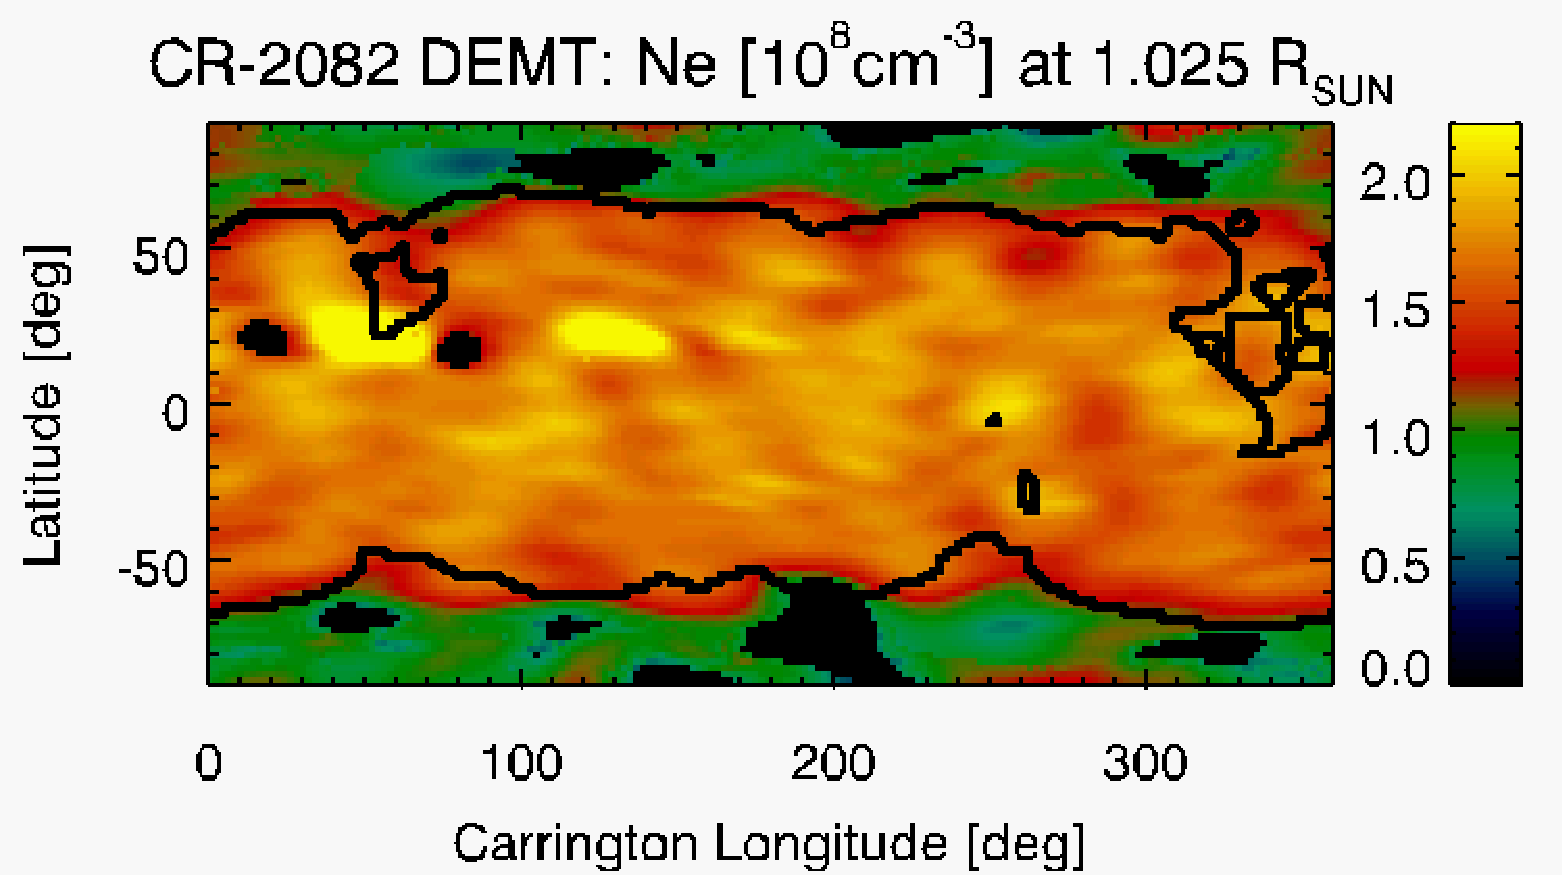
\includegraphics[width=0.495\textwidth]{figs/map_Ne_CR2082_DEMT-EUVI_behind_H1-L3523_r3d_1025_Rsun.pdf}
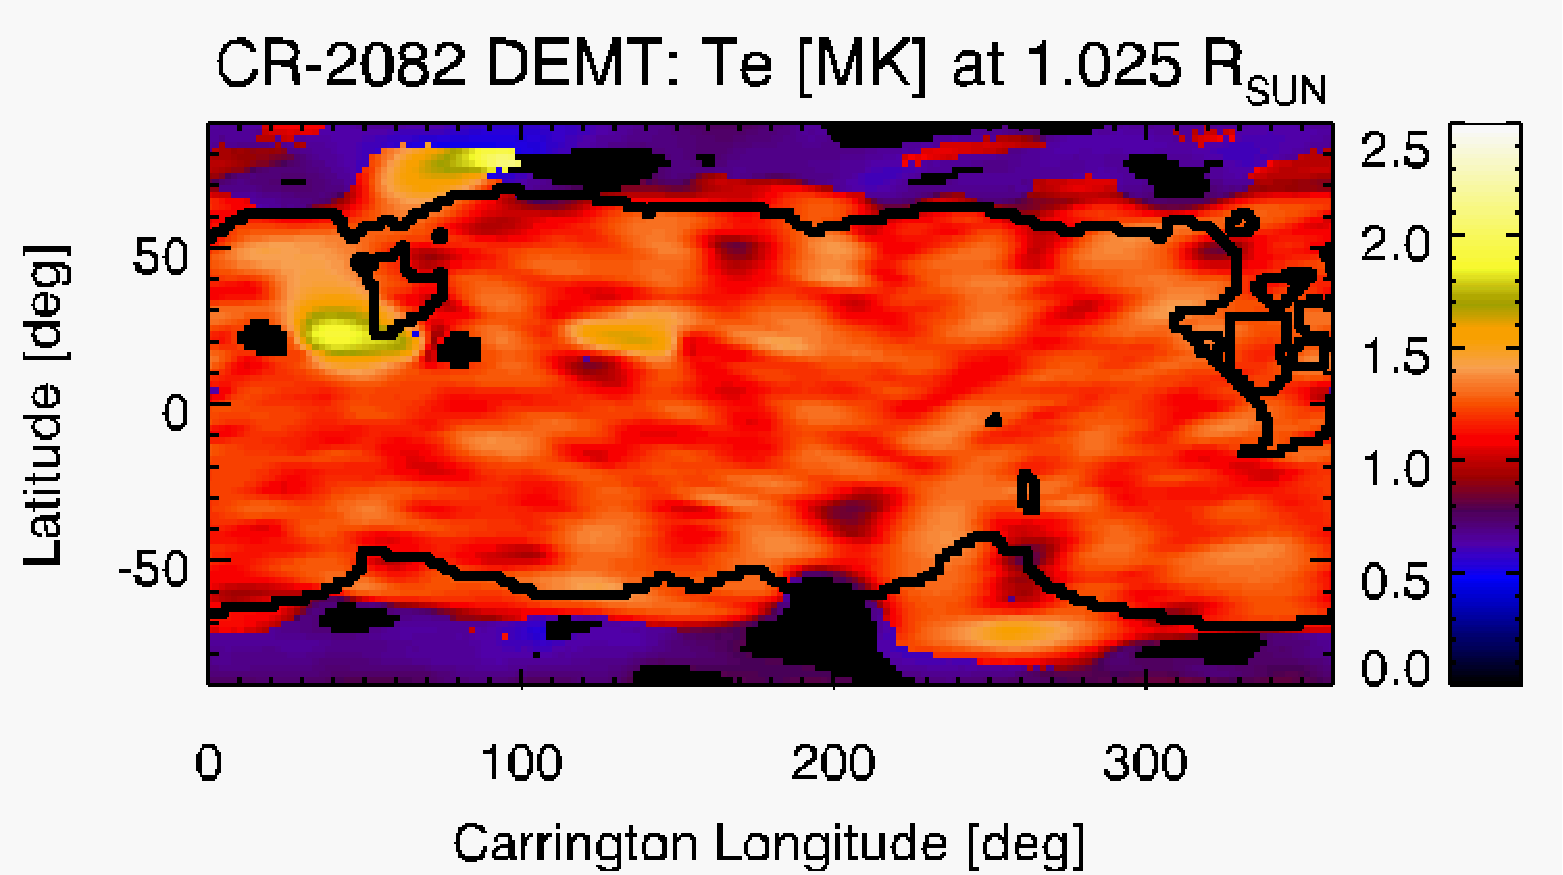
\includegraphics[width=0.495\textwidth]{figs/map_Tm_CR2082_DEMT-EUVI_behind_H1-L3523_r3d_1025_Rsun.pdf}
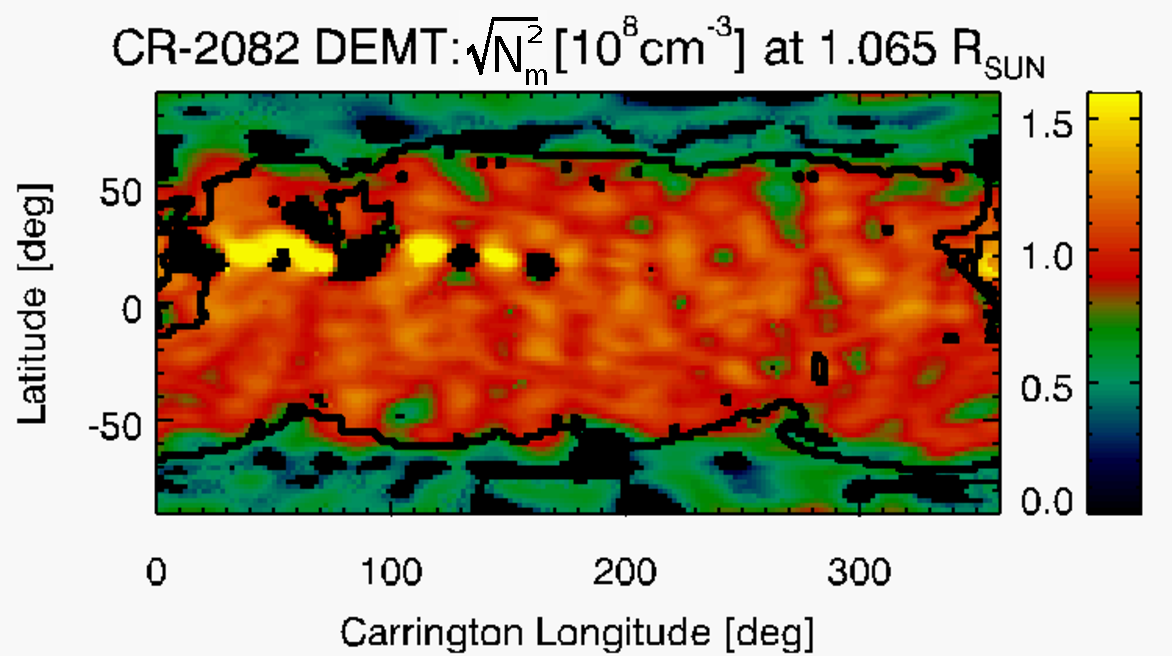
\includegraphics[width=0.495\textwidth]{figs/map_Ne_CR2082_DEMT-EUVI_behind_H1-L3523_r3d_1065_Rsun.pdf}
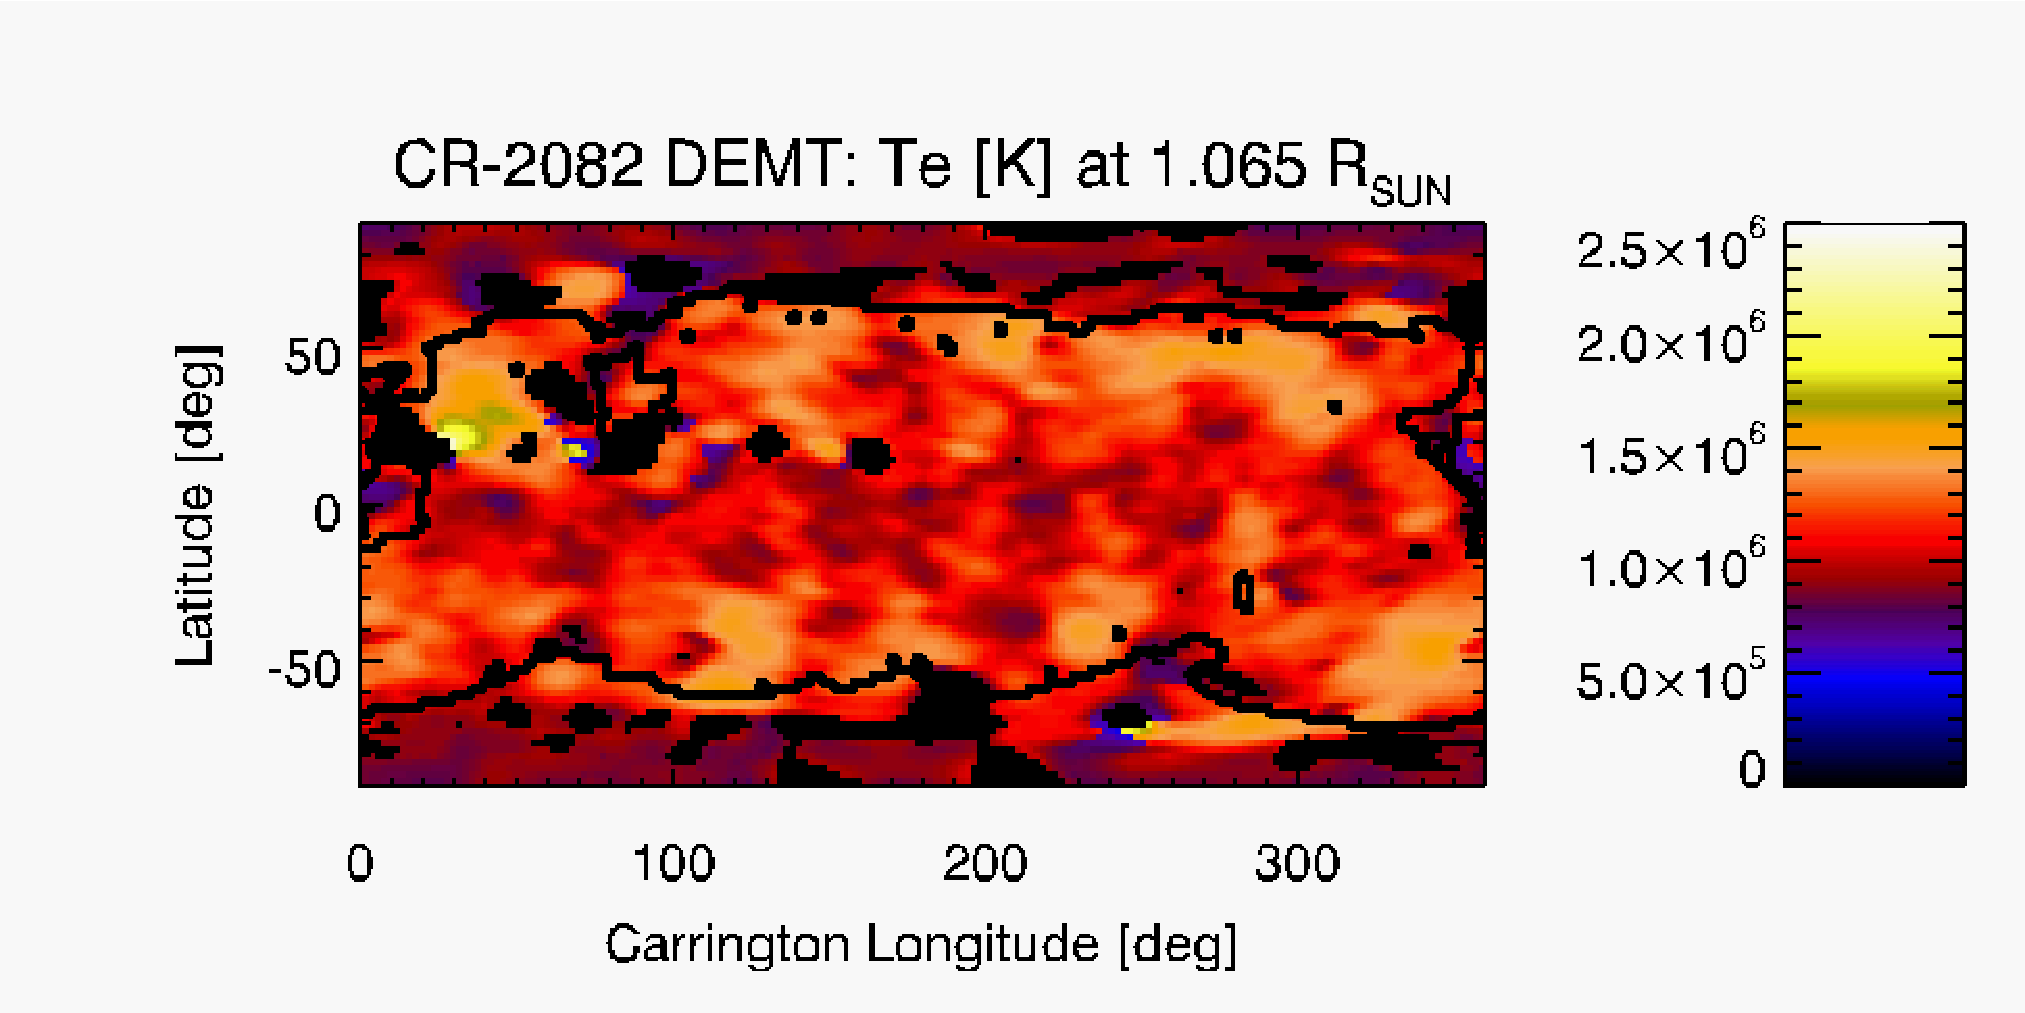
\includegraphics[width=0.495\textwidth]{figs/map_Tm_CR2082_DEMT-EUVI_behind_H1-L3523_r3d_1065_Rsun.pdf}
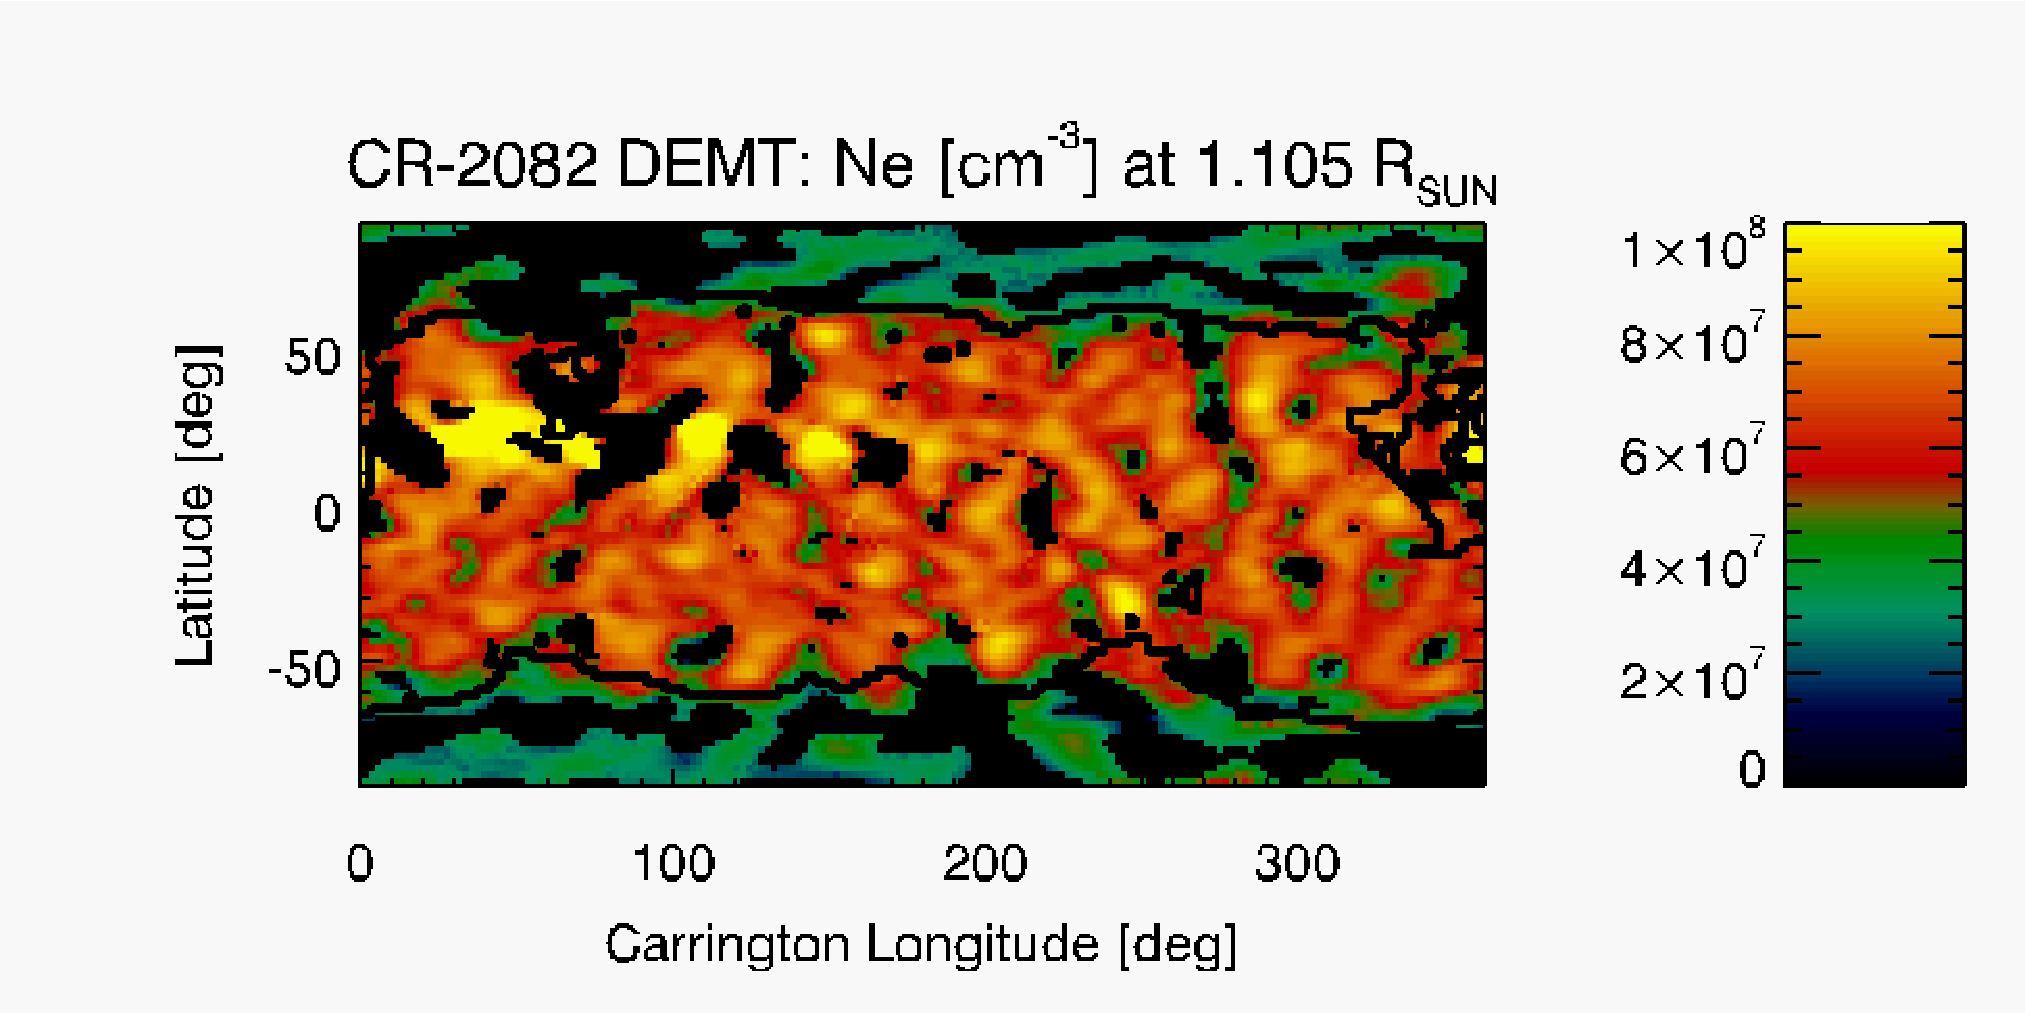
\includegraphics[width=0.495\textwidth]{figs/map_Ne_CR2082_DEMT-EUVI_behind_H1-L3523_r3d_1105_Rsun.pdf}
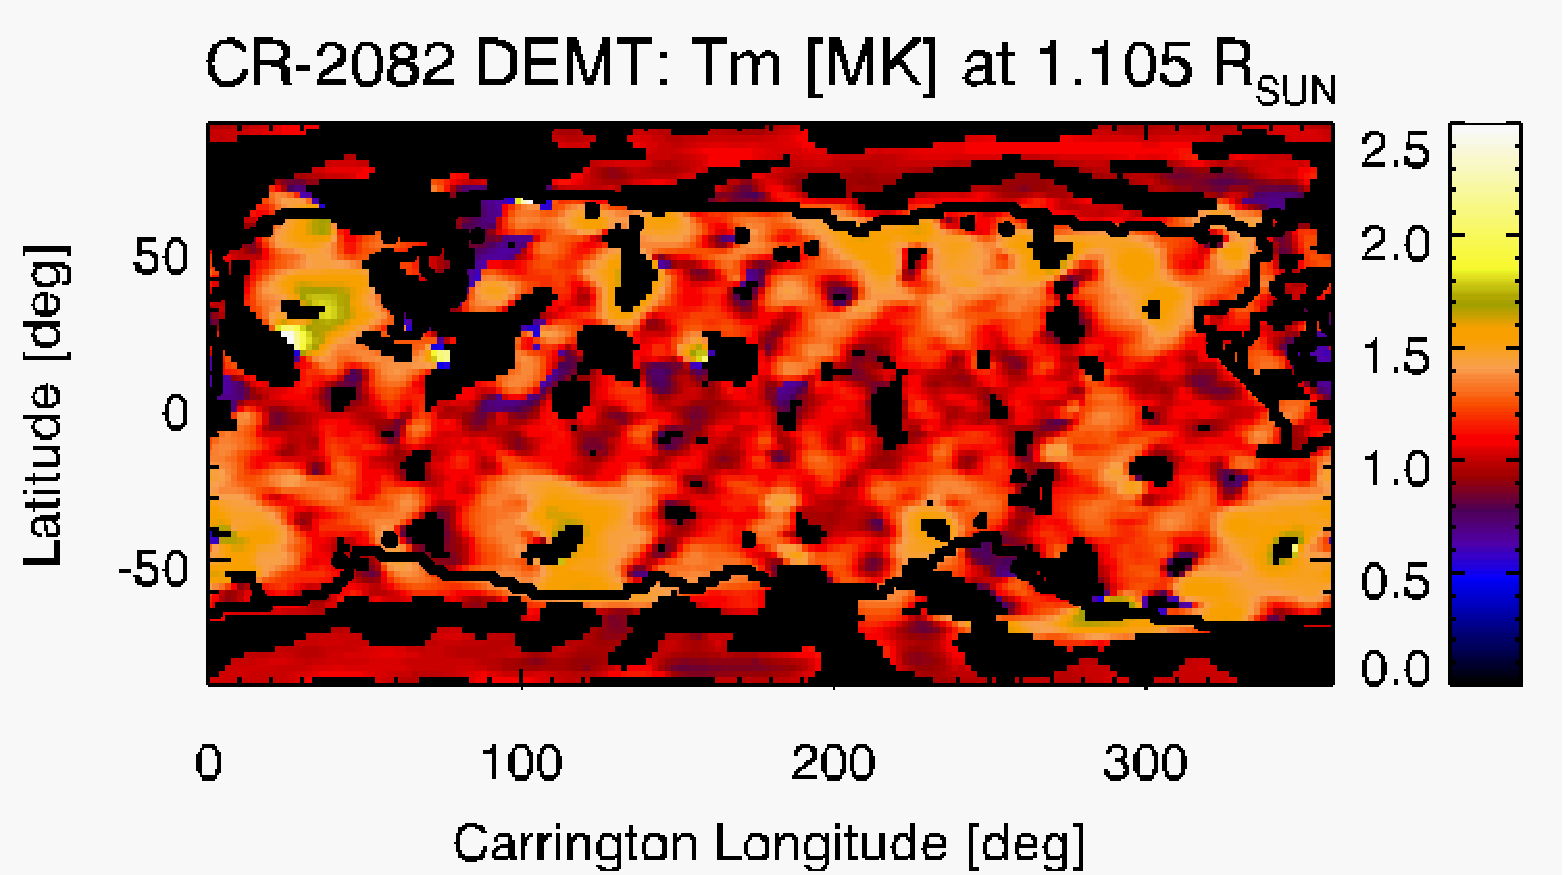
\includegraphics[width=0.495\textwidth]{figs/map_Tm_CR2082_DEMT-EUVI_behind_H1-L3523_r3d_1105_Rsun.pdf}
\caption{Carrington maps of DEMT {products $\sqravgN$} (left panels) and $\Tm$ (right panels) for CR-2082. Top, middle and bottom panels show the results at three heliocentric heights, $1.025$, $1.065$ and $1.105\,\mrsun$ respectively. Black voxels correspond to non-reconstructed regions (see text in Section \ref{demt_res}) and thick-black curves indicate the open/closed boundaries.}
\label{carmaps_demt_2082}
\end{center}
\end{figure}

{Both target rotations are highly axisymmetric, i.e. characterized by a high azymuthal symmetry. Rotation CR-2082} showed two {small} ARs (active {regions), both near latitude} $+30\mdeg$ and {around longitudes} $50\mdeg$ and $120\mdeg${, respectively}. {Rotation CR-2208} showed two {ARs, both near latitude} $+5\mdeg$ and {around longitudes $140\mdeg$ and $300\mdeg$, respectively.} 

{The magnetically open and closed regions of the AWSoM model are associated to CHs and the equatorial streamer belt, respectively. Consistently with that, the {location of the} open/closed boundaries derived from the respective AWSoM model quite accurately match {the regions of the DEMT maps which exhibit the strongest latitudinal gradient of both the electron density and temperature.}}

\begin{figure}[h!]
\begin{center}
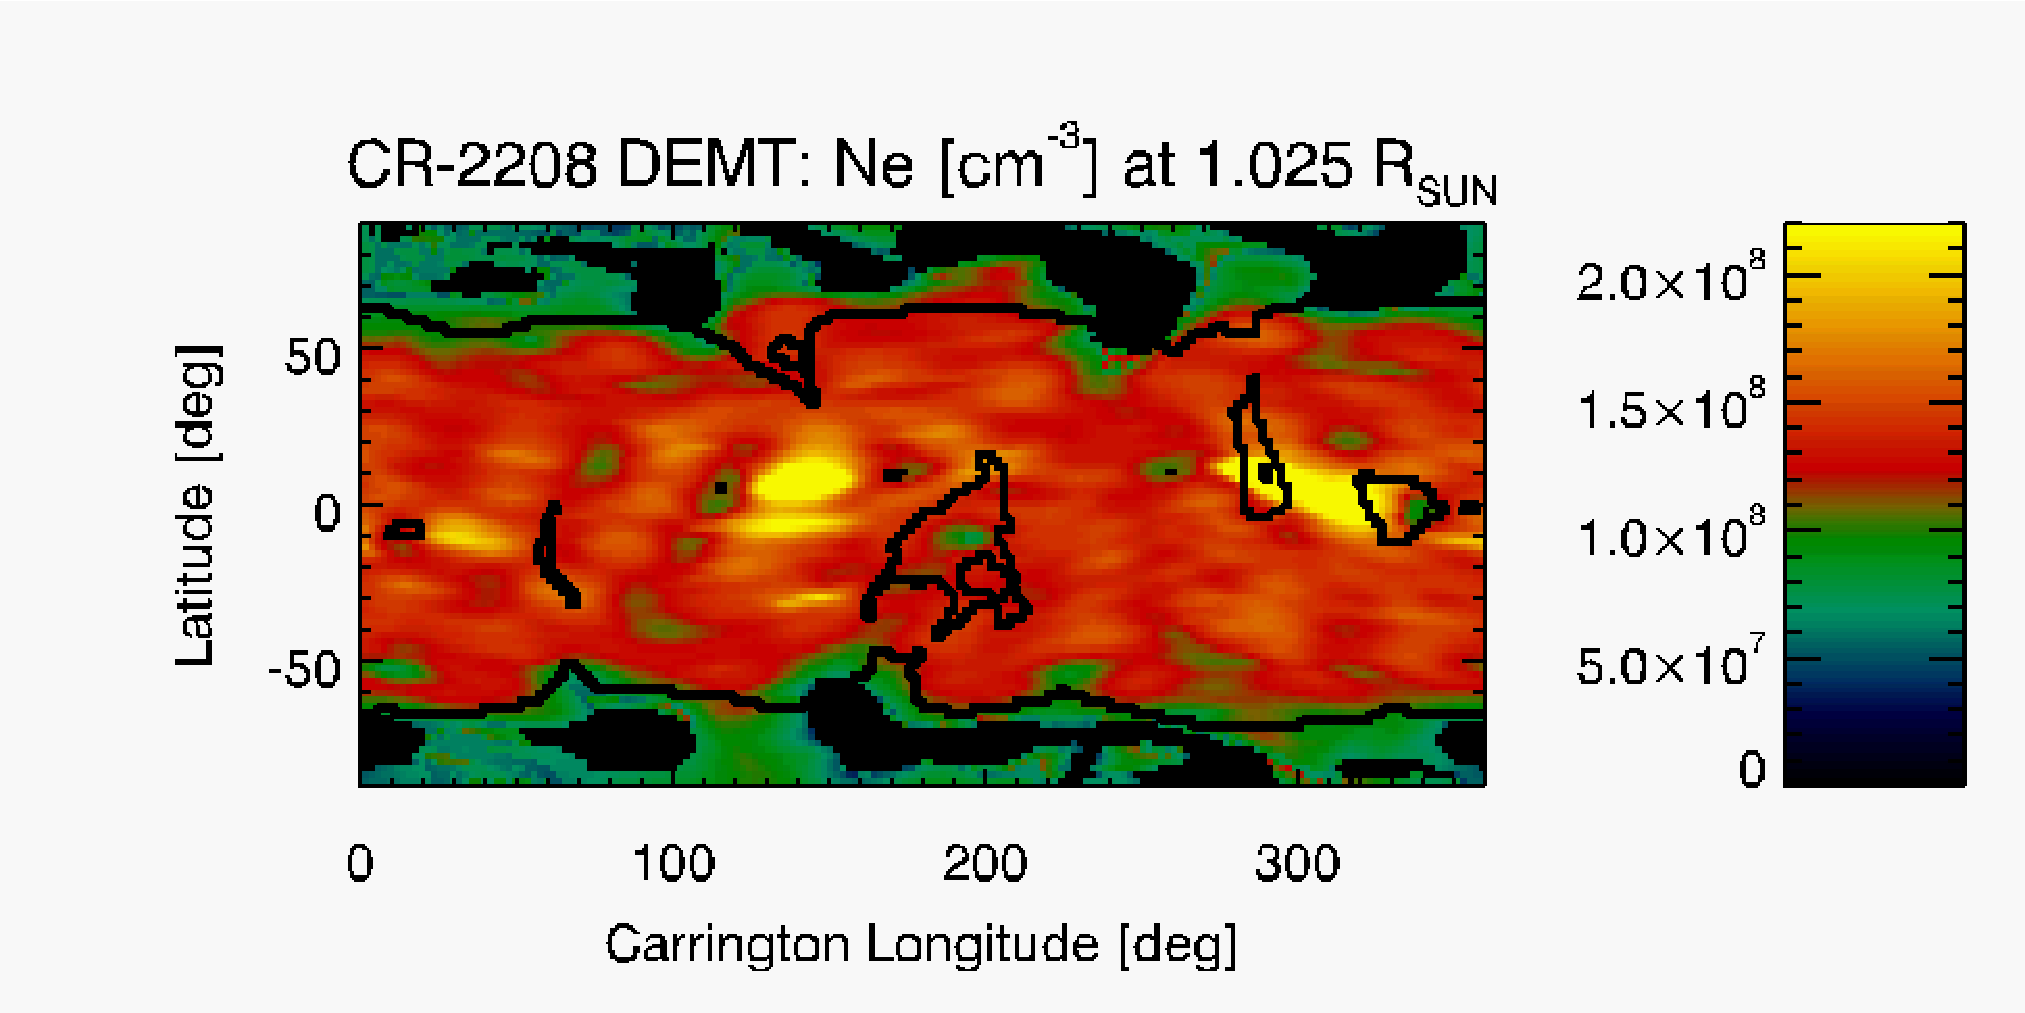
\includegraphics[width=0.495\textwidth]{figs/map_Ne_CR2208_DEMT-AIA_H1_L522_r3d_1025_Rsun.pdf}
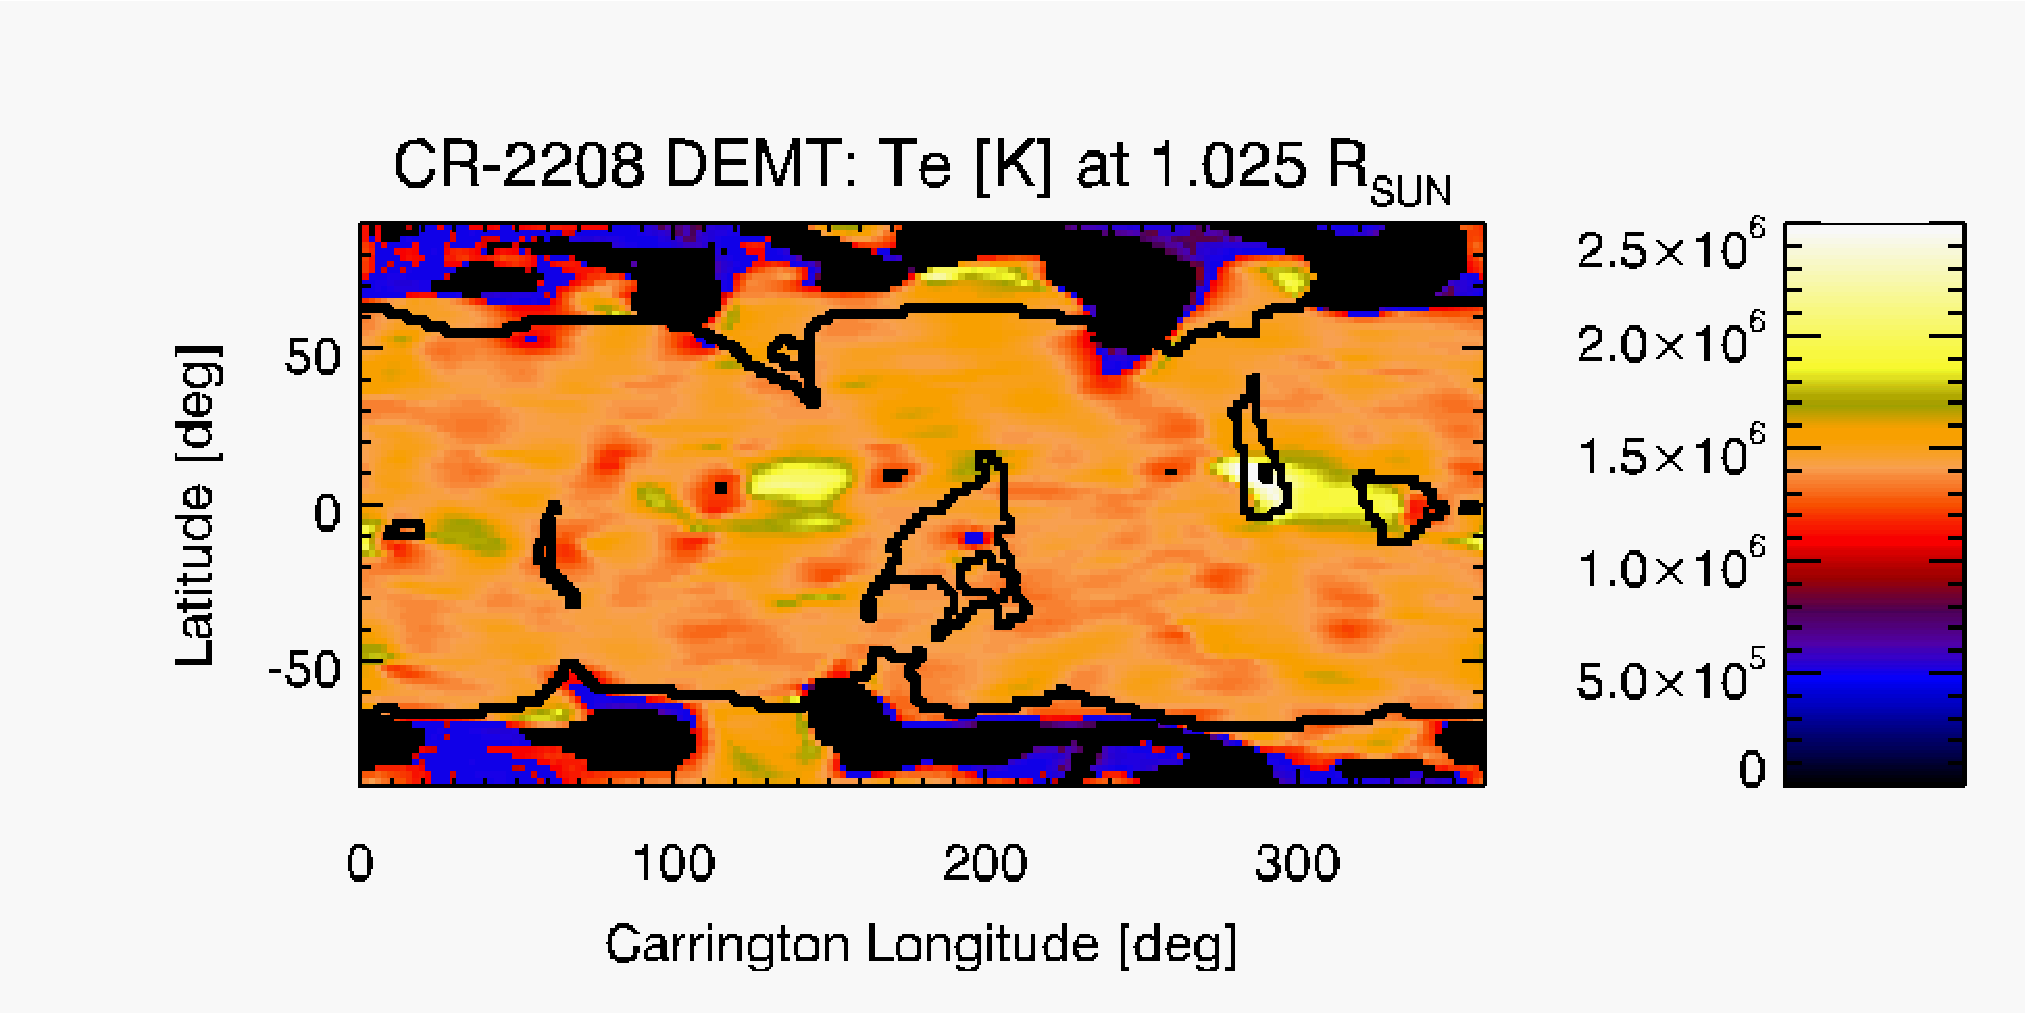
\includegraphics[width=0.495\textwidth]{figs/map_Tm_CR2208_DEMT-AIA_H1_L522_r3d_1025_Rsun.pdf}
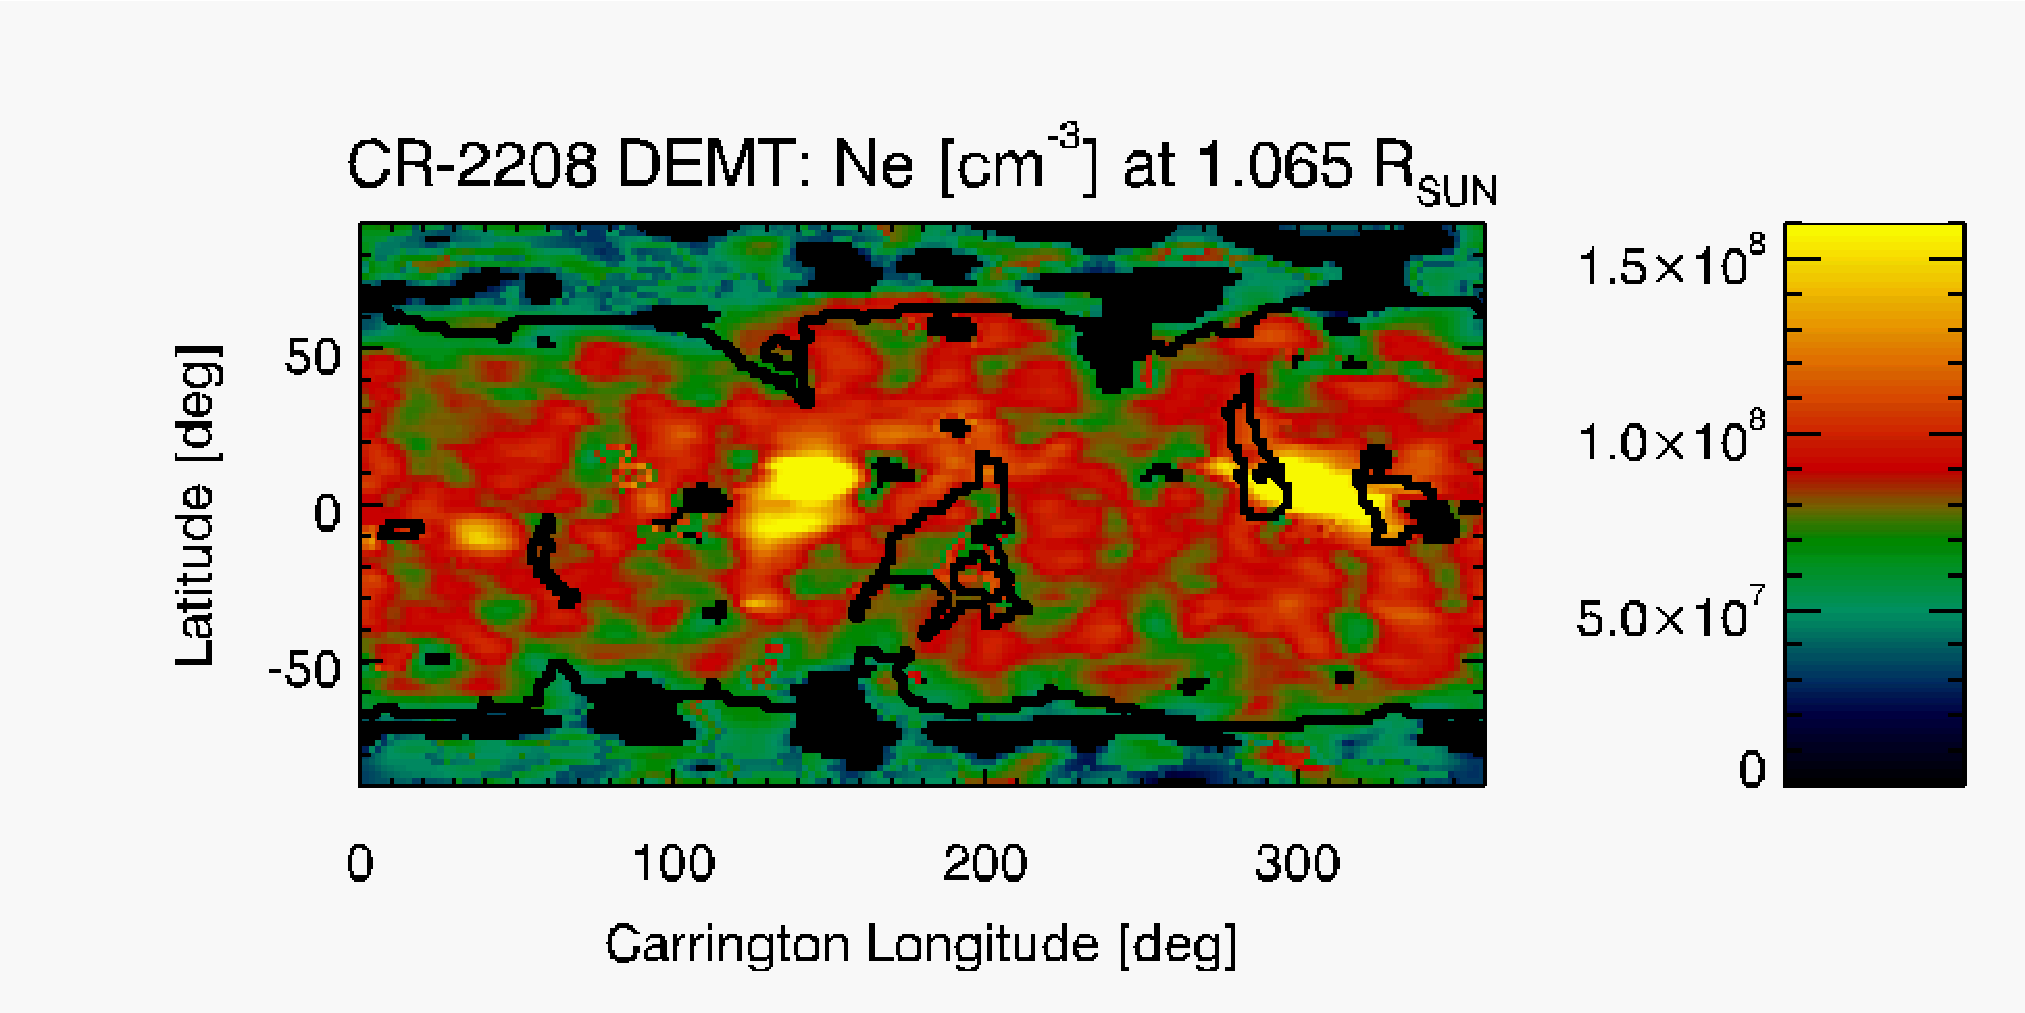
\includegraphics[width=0.495\textwidth]{figs/map_Ne_CR2208_DEMT-AIA_H1_L522_r3d_1065_Rsun.pdf}
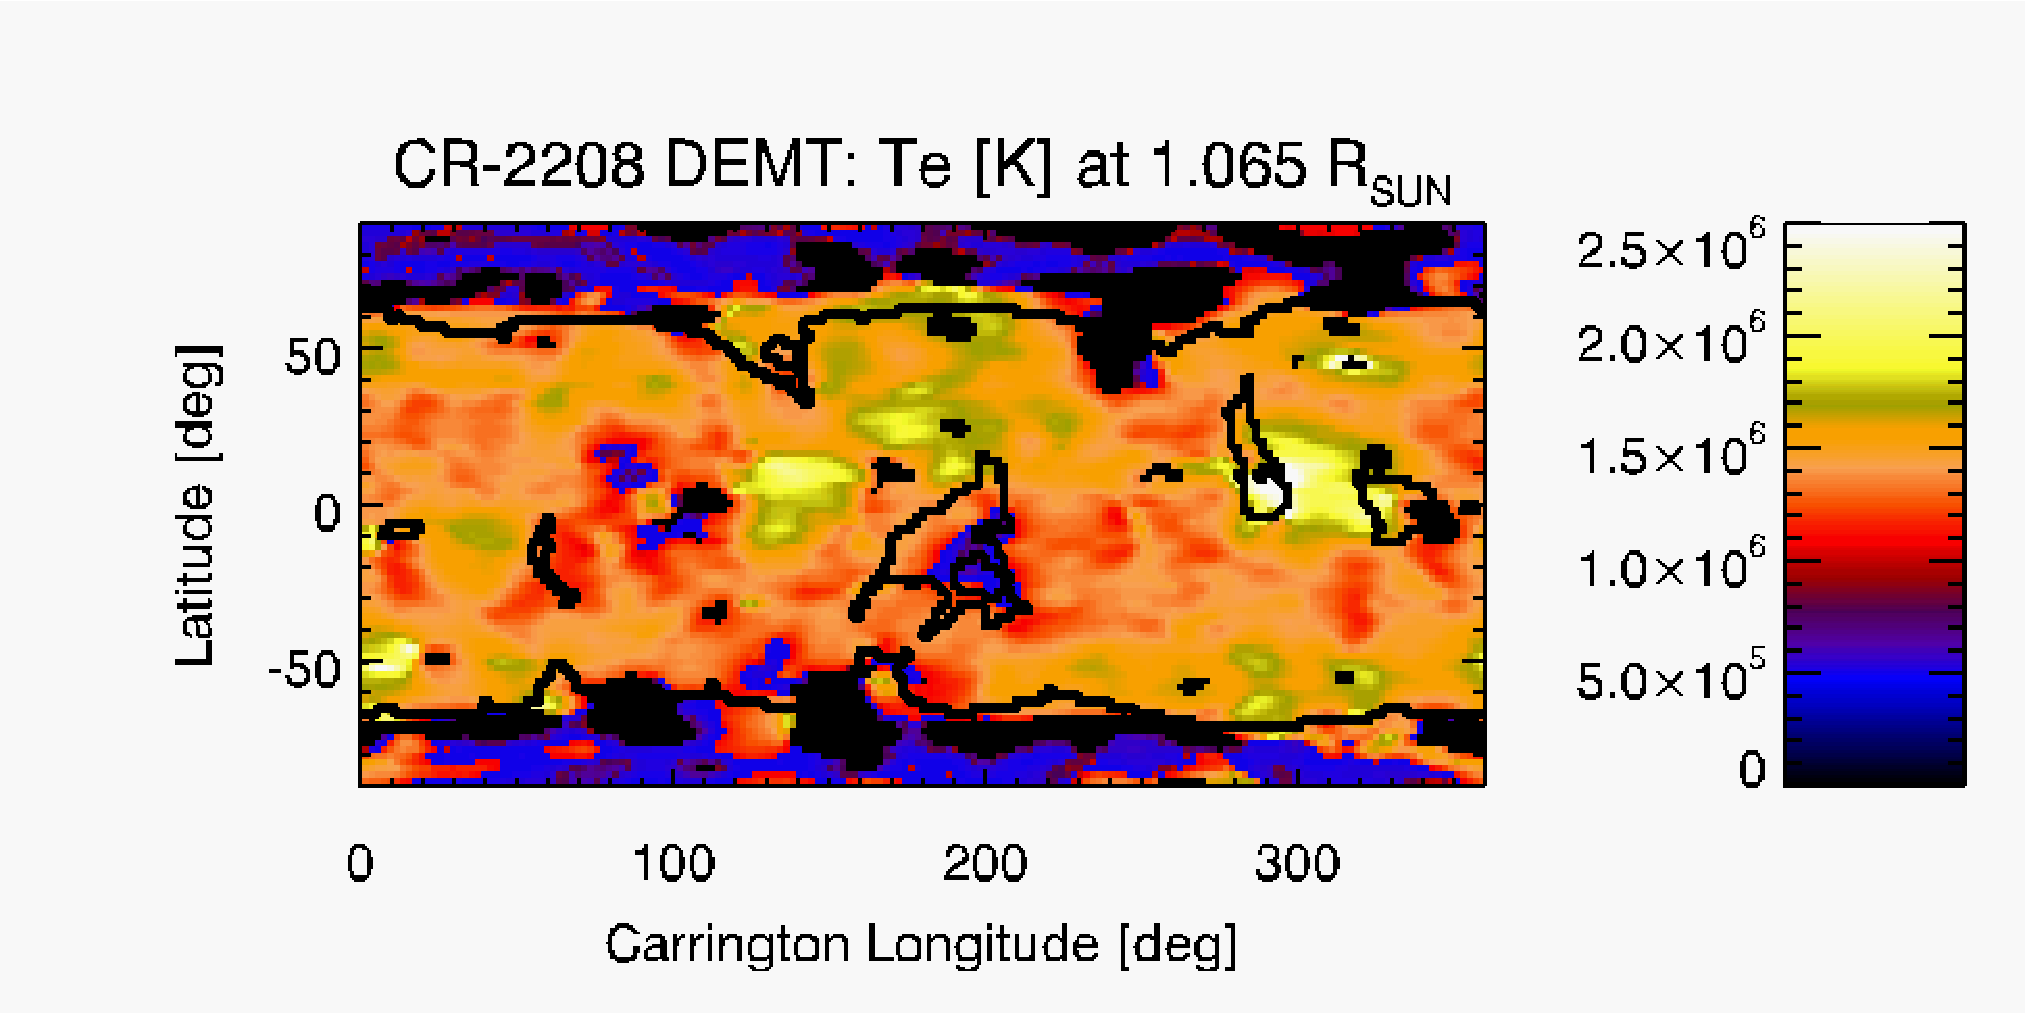
\includegraphics[width=0.495\textwidth]{figs/map_Tm_CR2208_DEMT-AIA_H1_L522_r3d_1065_Rsun.pdf}
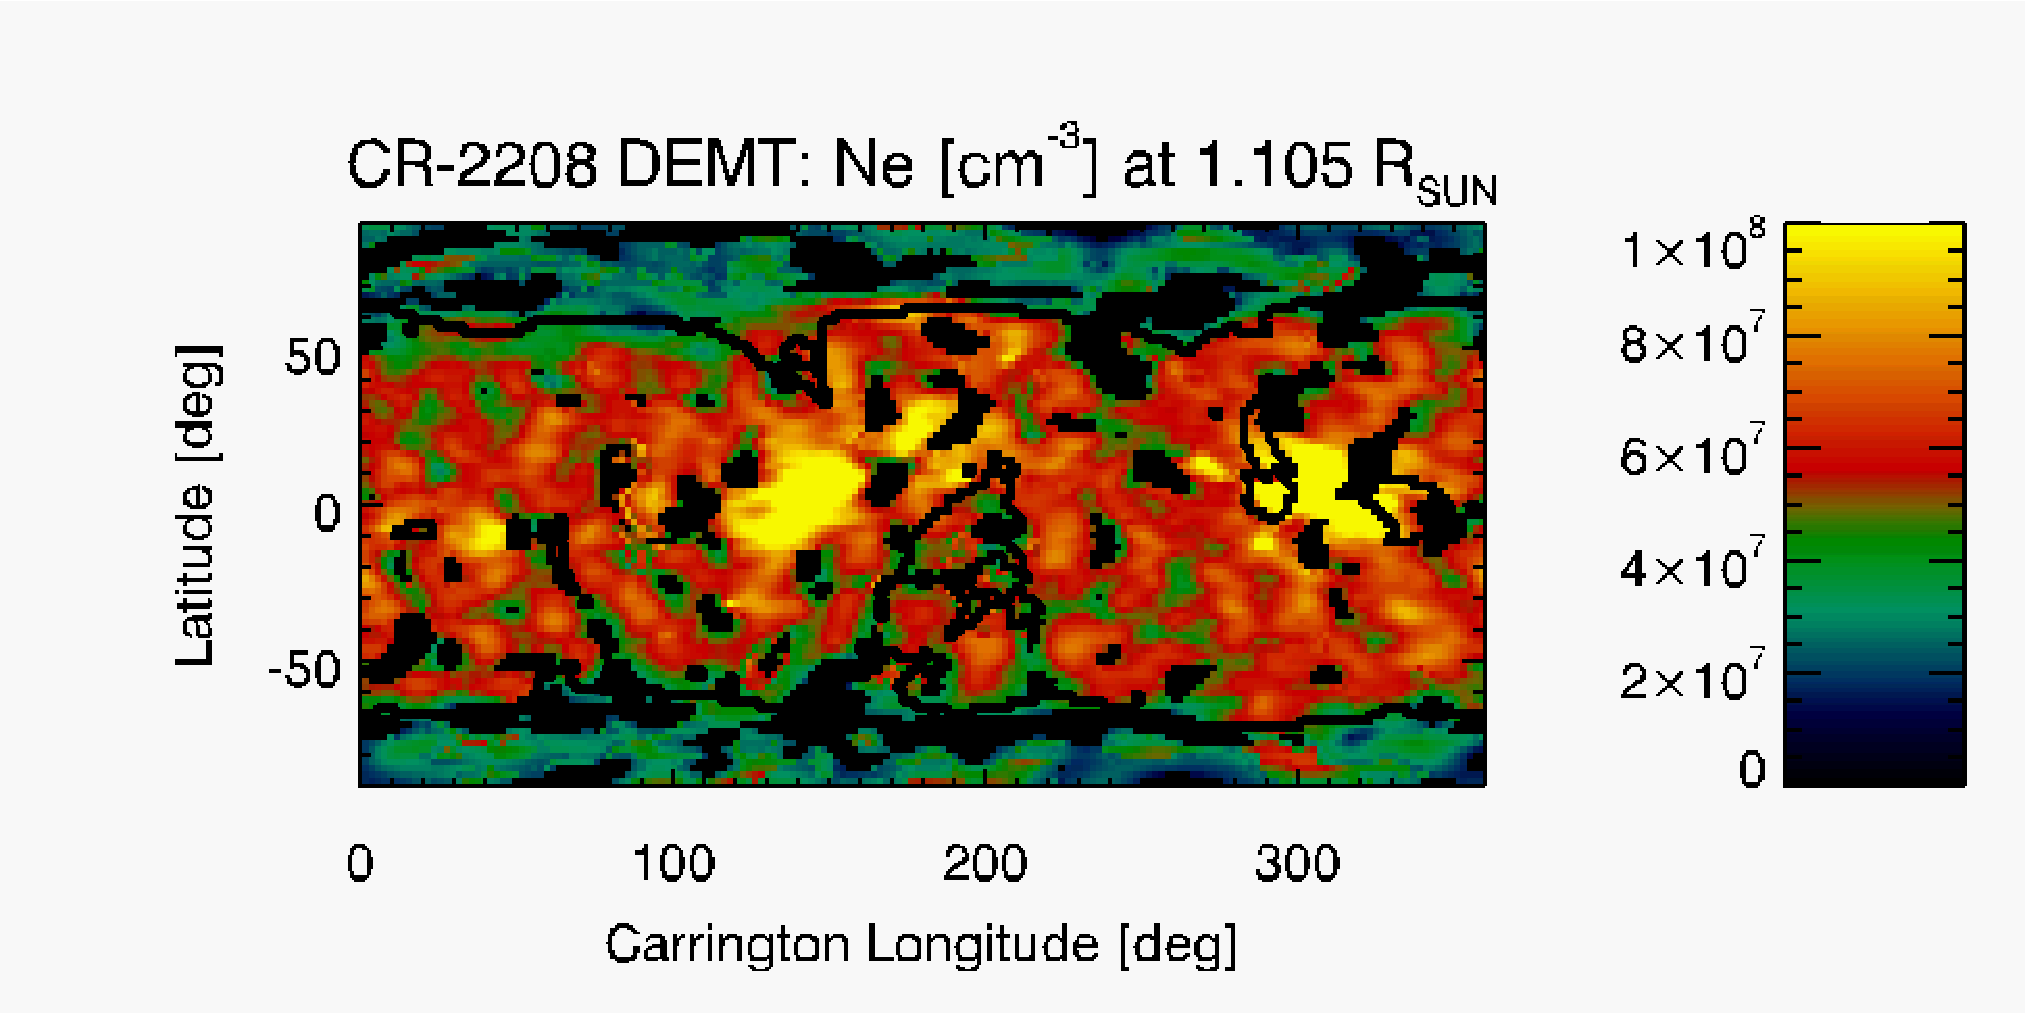
\includegraphics[width=0.495\textwidth]{figs/map_Ne_CR2208_DEMT-AIA_H1_L522_r3d_1105_Rsun.pdf}
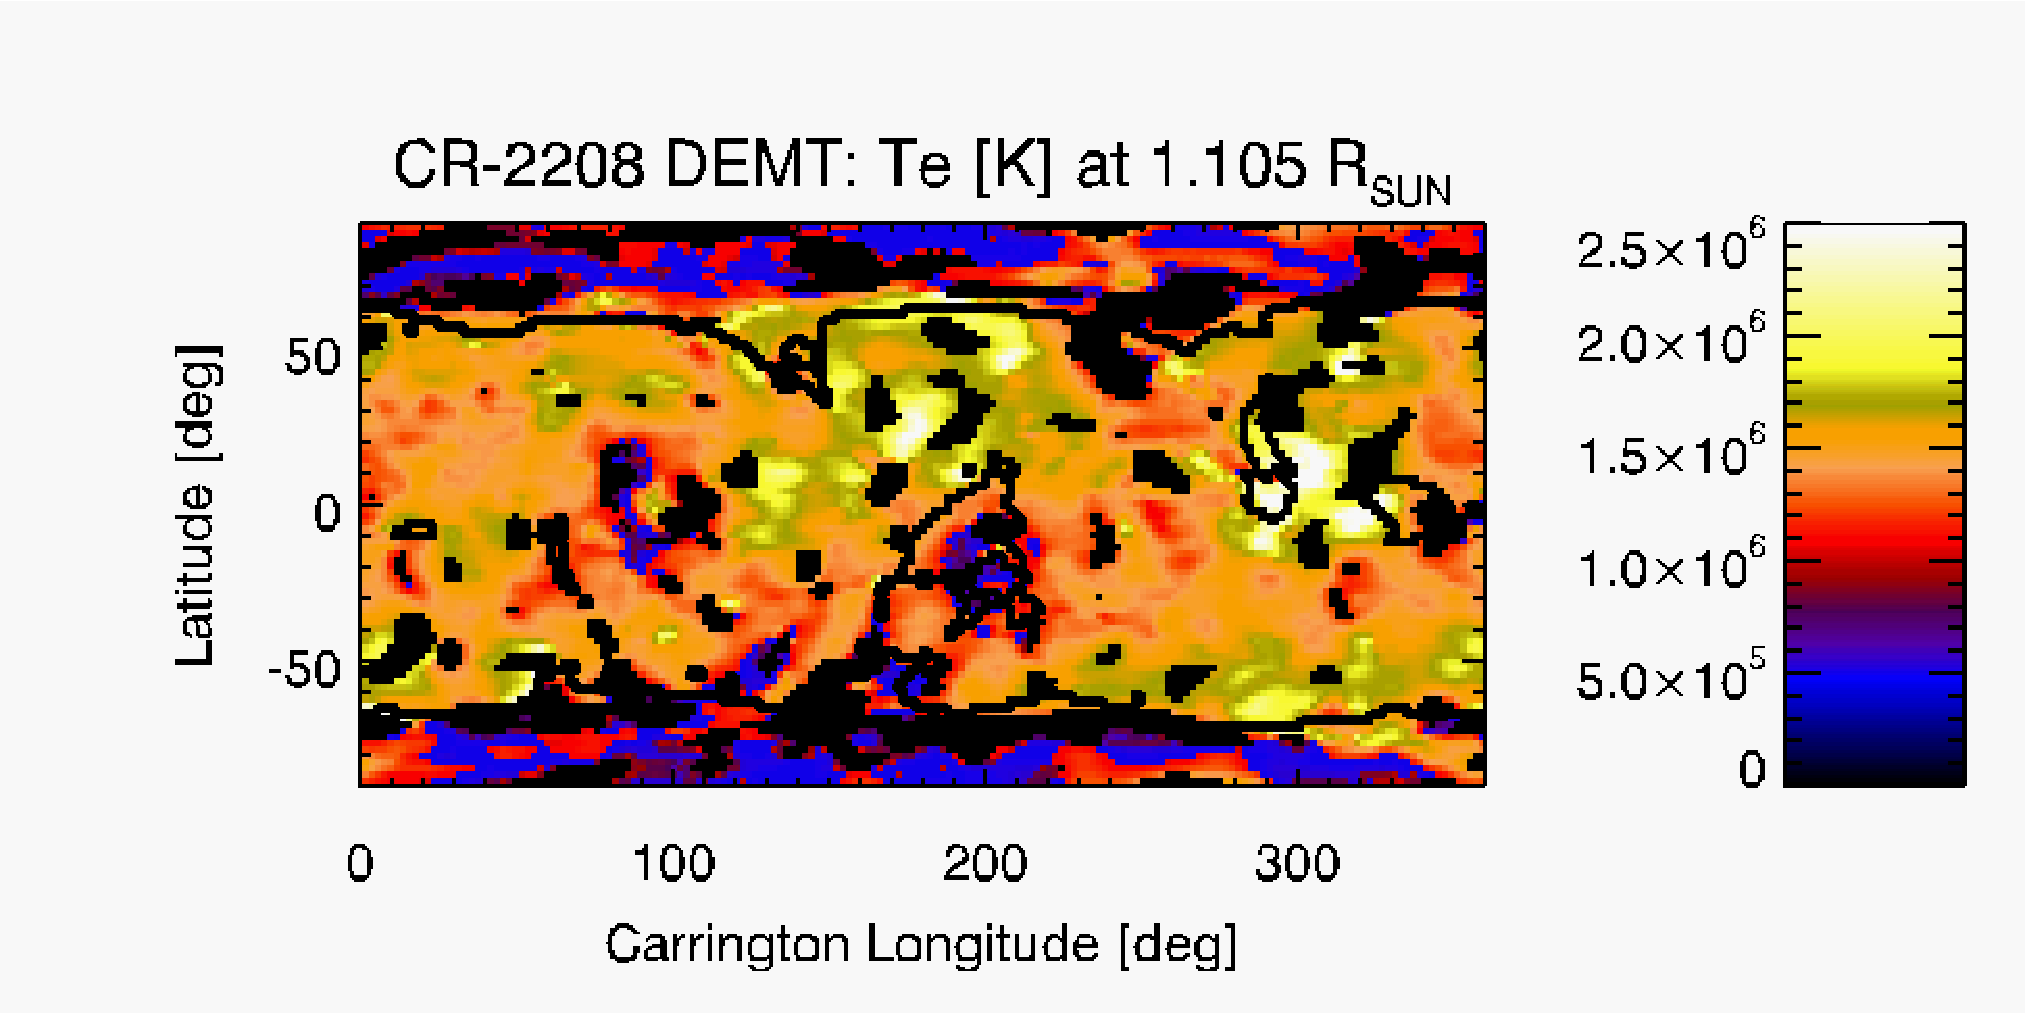
\includegraphics[width=0.495\textwidth]{figs/map_Tm_CR2208_DEMT-AIA_H1_L522_r3d_1105_Rsun.pdf}
\caption{Same as Figure \ref{carmaps_demt_2082} but for CR-2208.}
\label{carmaps_demt_2208}
\end{center}
\end{figure}

{{Figures \ref{carmaps_demt_2082} and \ref{carmaps_demt_2208} show that} the DEMT reconstruction of the streamer belt is characterized by relatively larger values of density and temperature in comparison to the CHs. They also show that the streamer belt region of CR-2082 was denser and colder than  that of CR-2208.} In the case of CR-2082, which belongs to the deep minimum epoch between {SCs 24 and 25}, the {low latitudes of the streamer belt are characterized by lower electron temperature than in its mid-latitudes.} A similar behavior is seen in CR-2208, belonging to the declining phase of {SC 25, but having a {somewhat less axisymmetric} structure this characteristic is not so obvious. This thermodynamic structure} of the streamer have been reported for other solar minimum rotations in previous DEMT works \citep{lloveras_2017,nuevo_2013,vasquez_2010}.

{For both target rotations, Figure \ref{carmaps_R_2082_2208} shows {latitude-longitude} maps of {the DEMT} measure $R$ defined by Equation (\ref{R}), at the same three heights shown in Figures \ref{momento1} and \ref{momento2}. In most of the coronal volume of the DEMT grid the agreement between the tomographic and synthetic FBEs is $\lesssim 1\%$. The notable exception is to be found in the CHs of the target rotation {analysed} based on AIA data. A similar results was found in the two existing DEMT works based on data provided by the AIA instrument \citep{nuevo_2015,maccormack_2017}. This point is further discussed below.}

\begin{figure}[h!]
\begin{center}
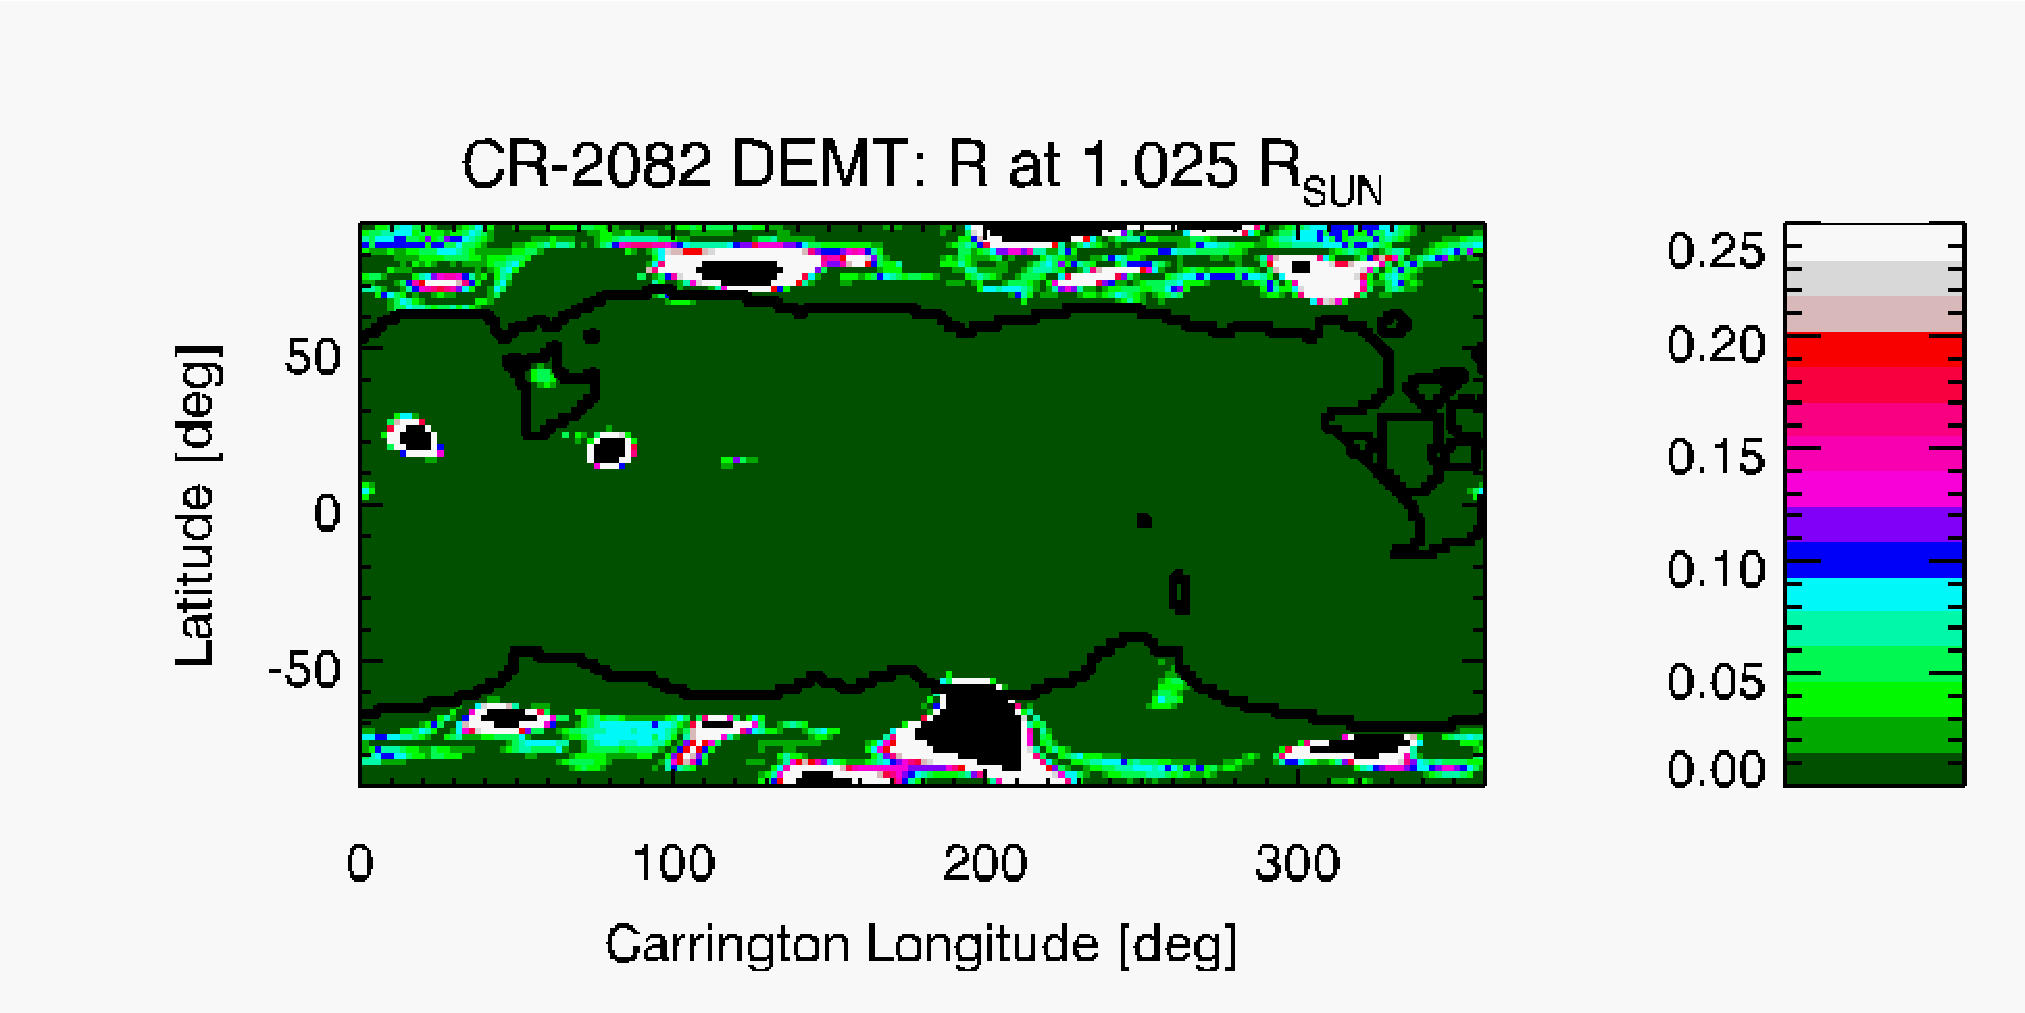
\includegraphics[width=0.495\textwidth]{figs/map_R_CR2082_DEMT-EUVI_behind_H1-L3523_r3d_1025_Rsun.pdf}
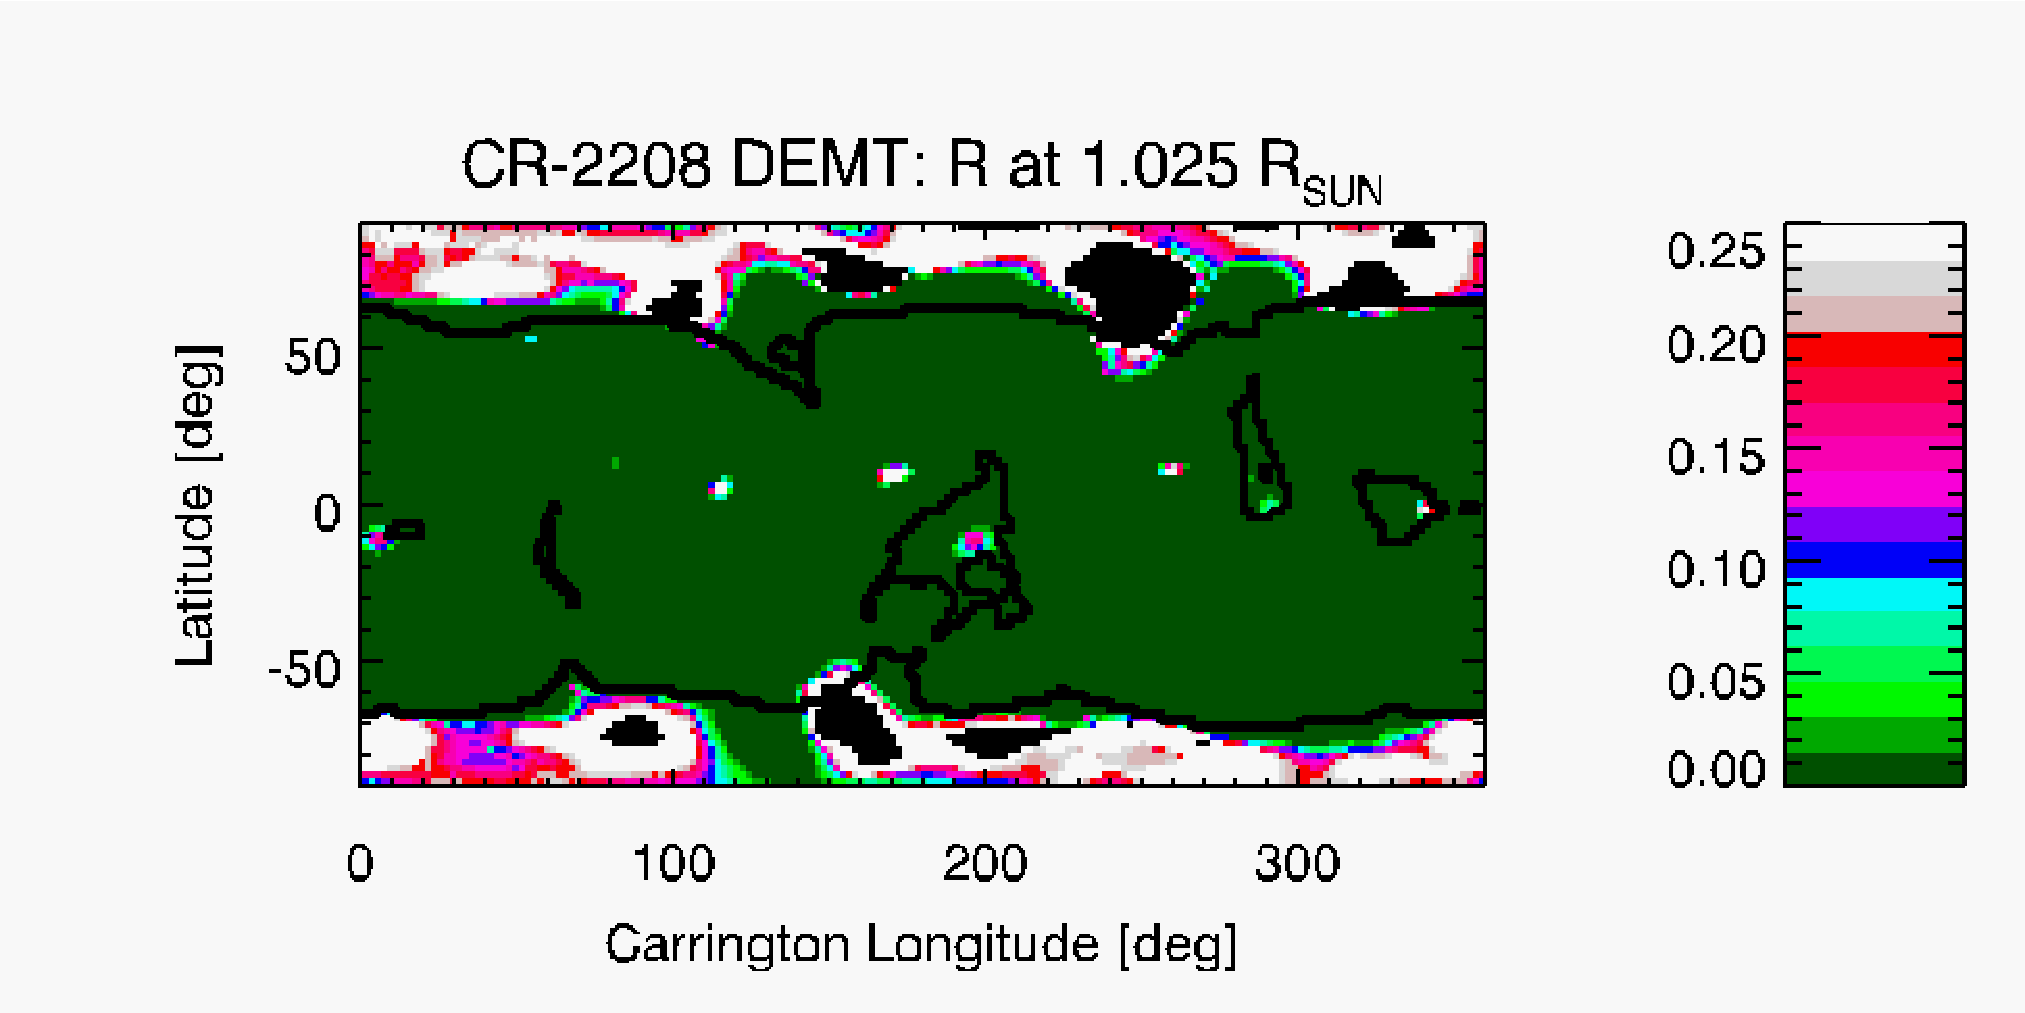
\includegraphics[width=0.495\textwidth]{figs/map_R_CR2208_DEMT-AIA_H1_L522_r3d_1025_Rsun.pdf}
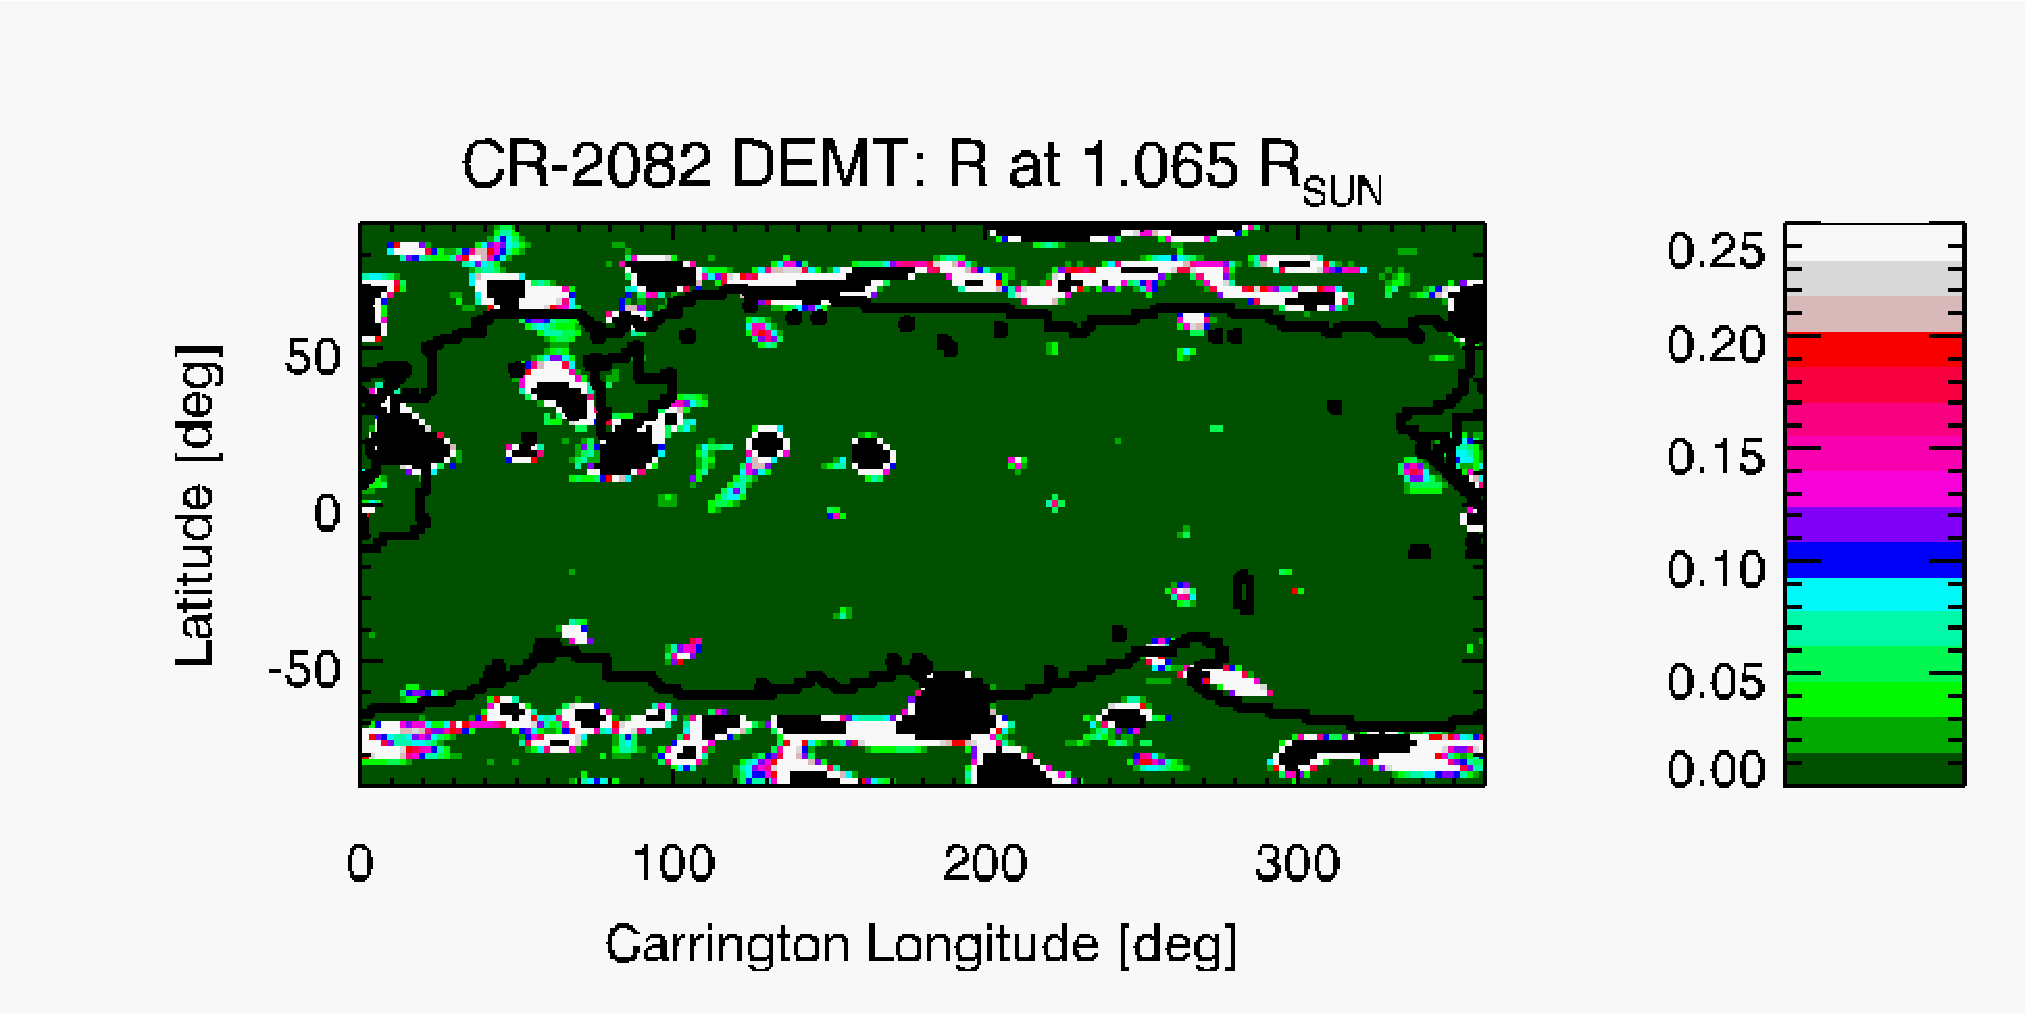
\includegraphics[width=0.495\textwidth]{figs/map_R_CR2082_DEMT-EUVI_behind_H1-L3523_r3d_1065_Rsun.pdf}
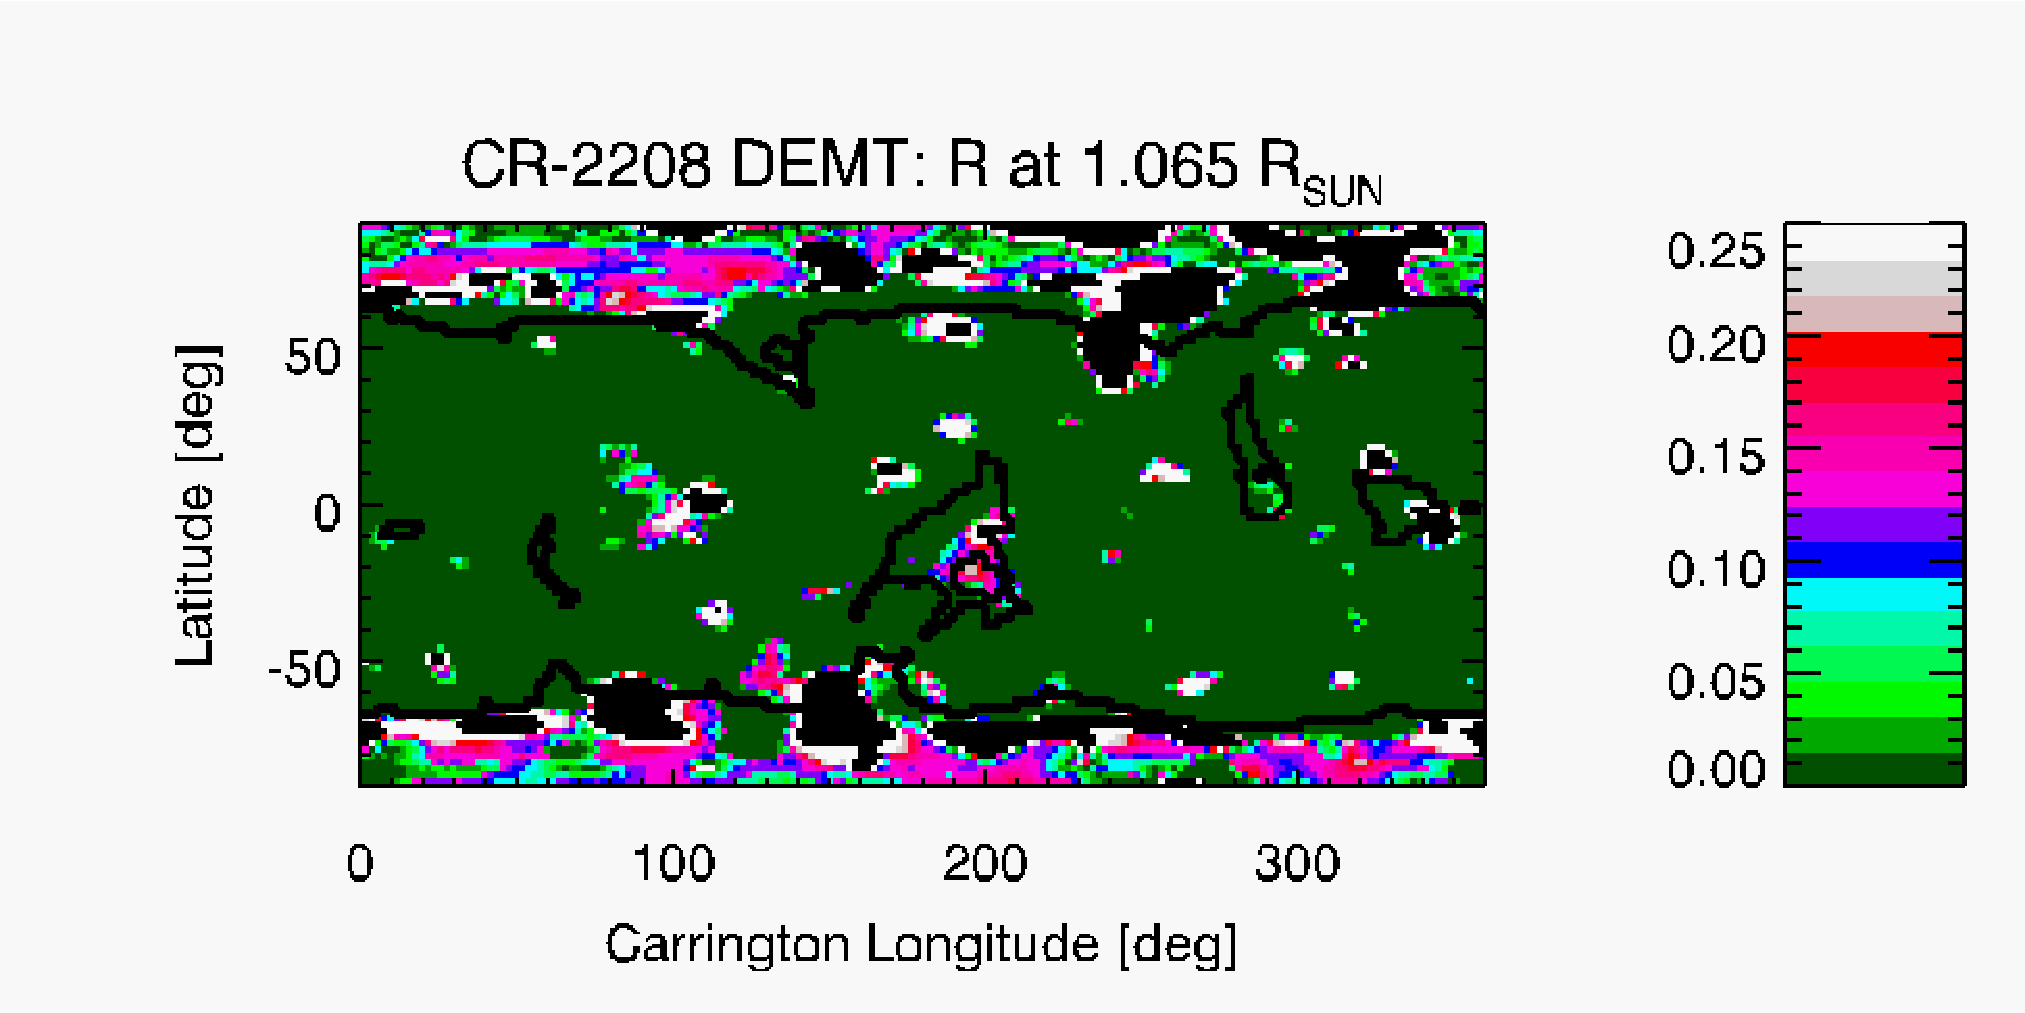
\includegraphics[width=0.495\textwidth]{figs/map_R_CR2208_DEMT-AIA_H1_L522_r3d_1065_Rsun.pdf}
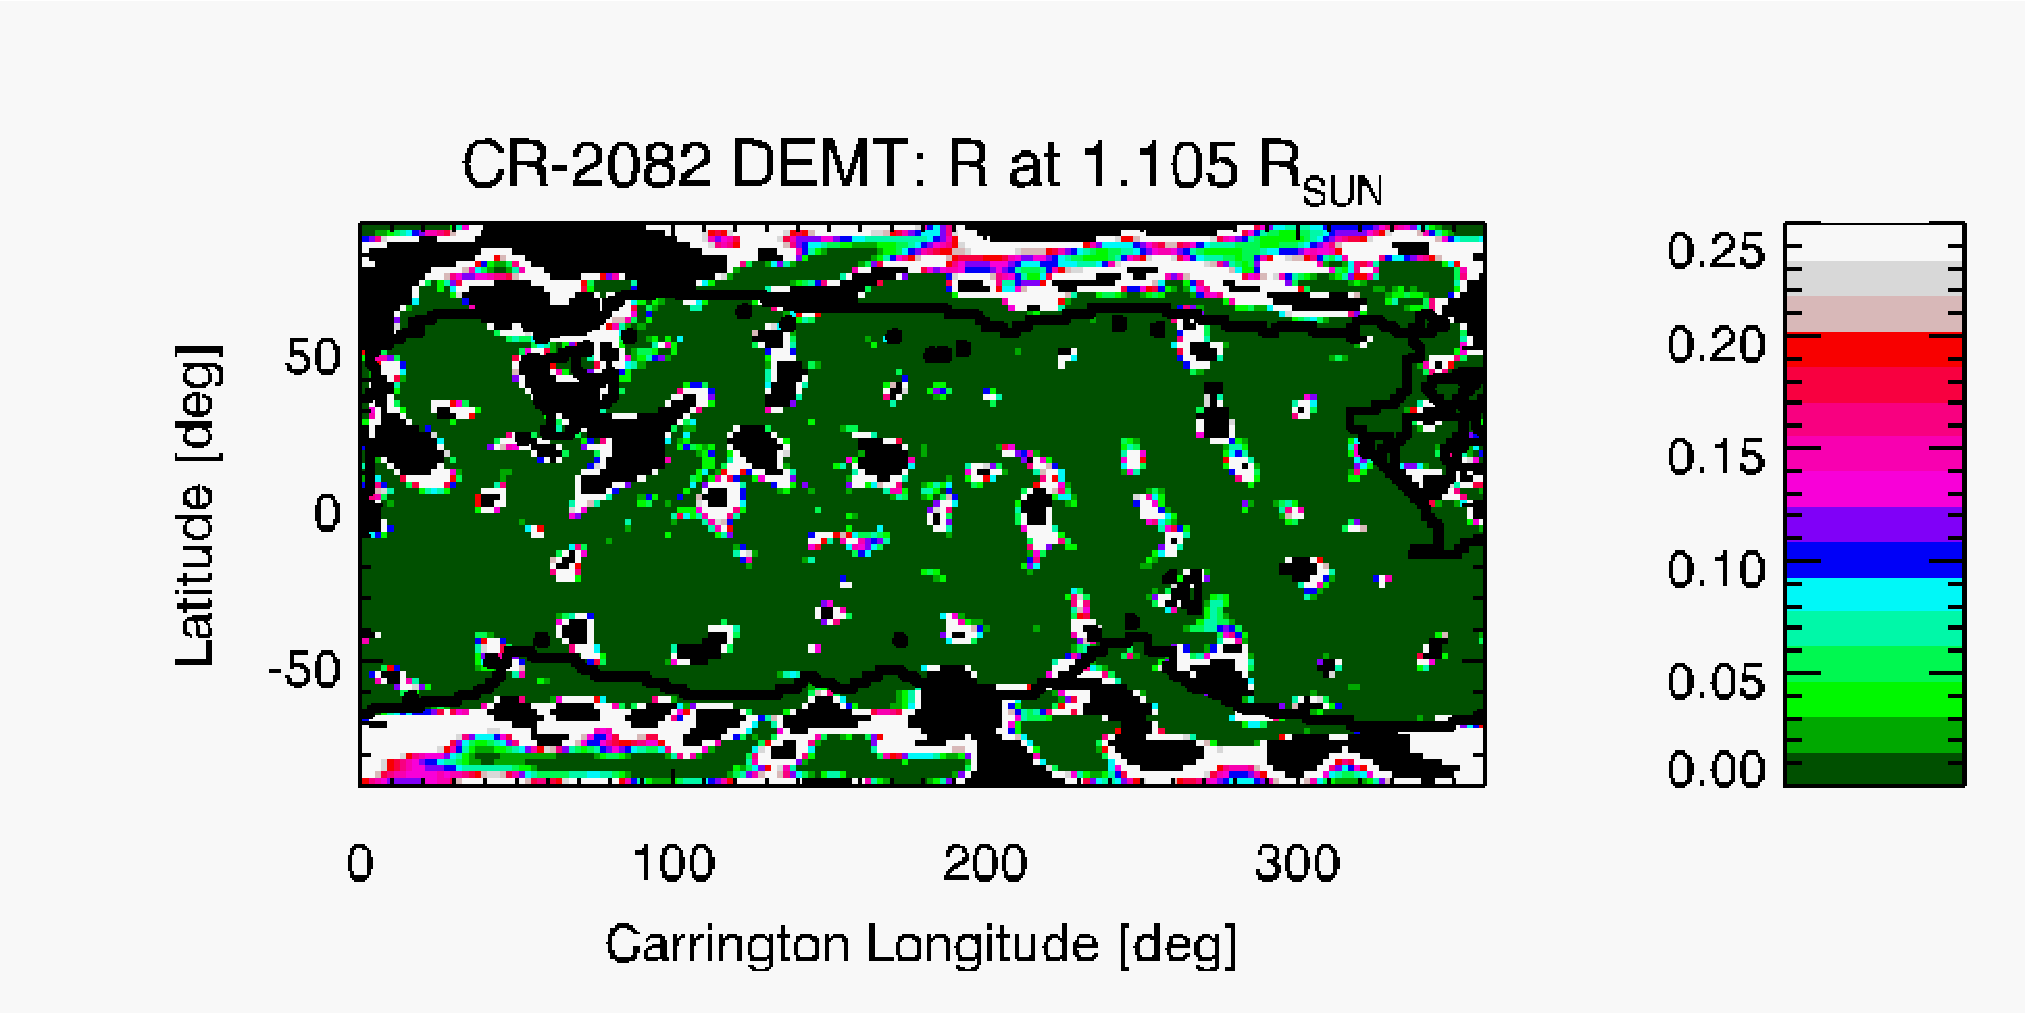
\includegraphics[width=0.495\textwidth]{figs/map_R_CR2082_DEMT-EUVI_behind_H1-L3523_r3d_1105_Rsun.pdf}
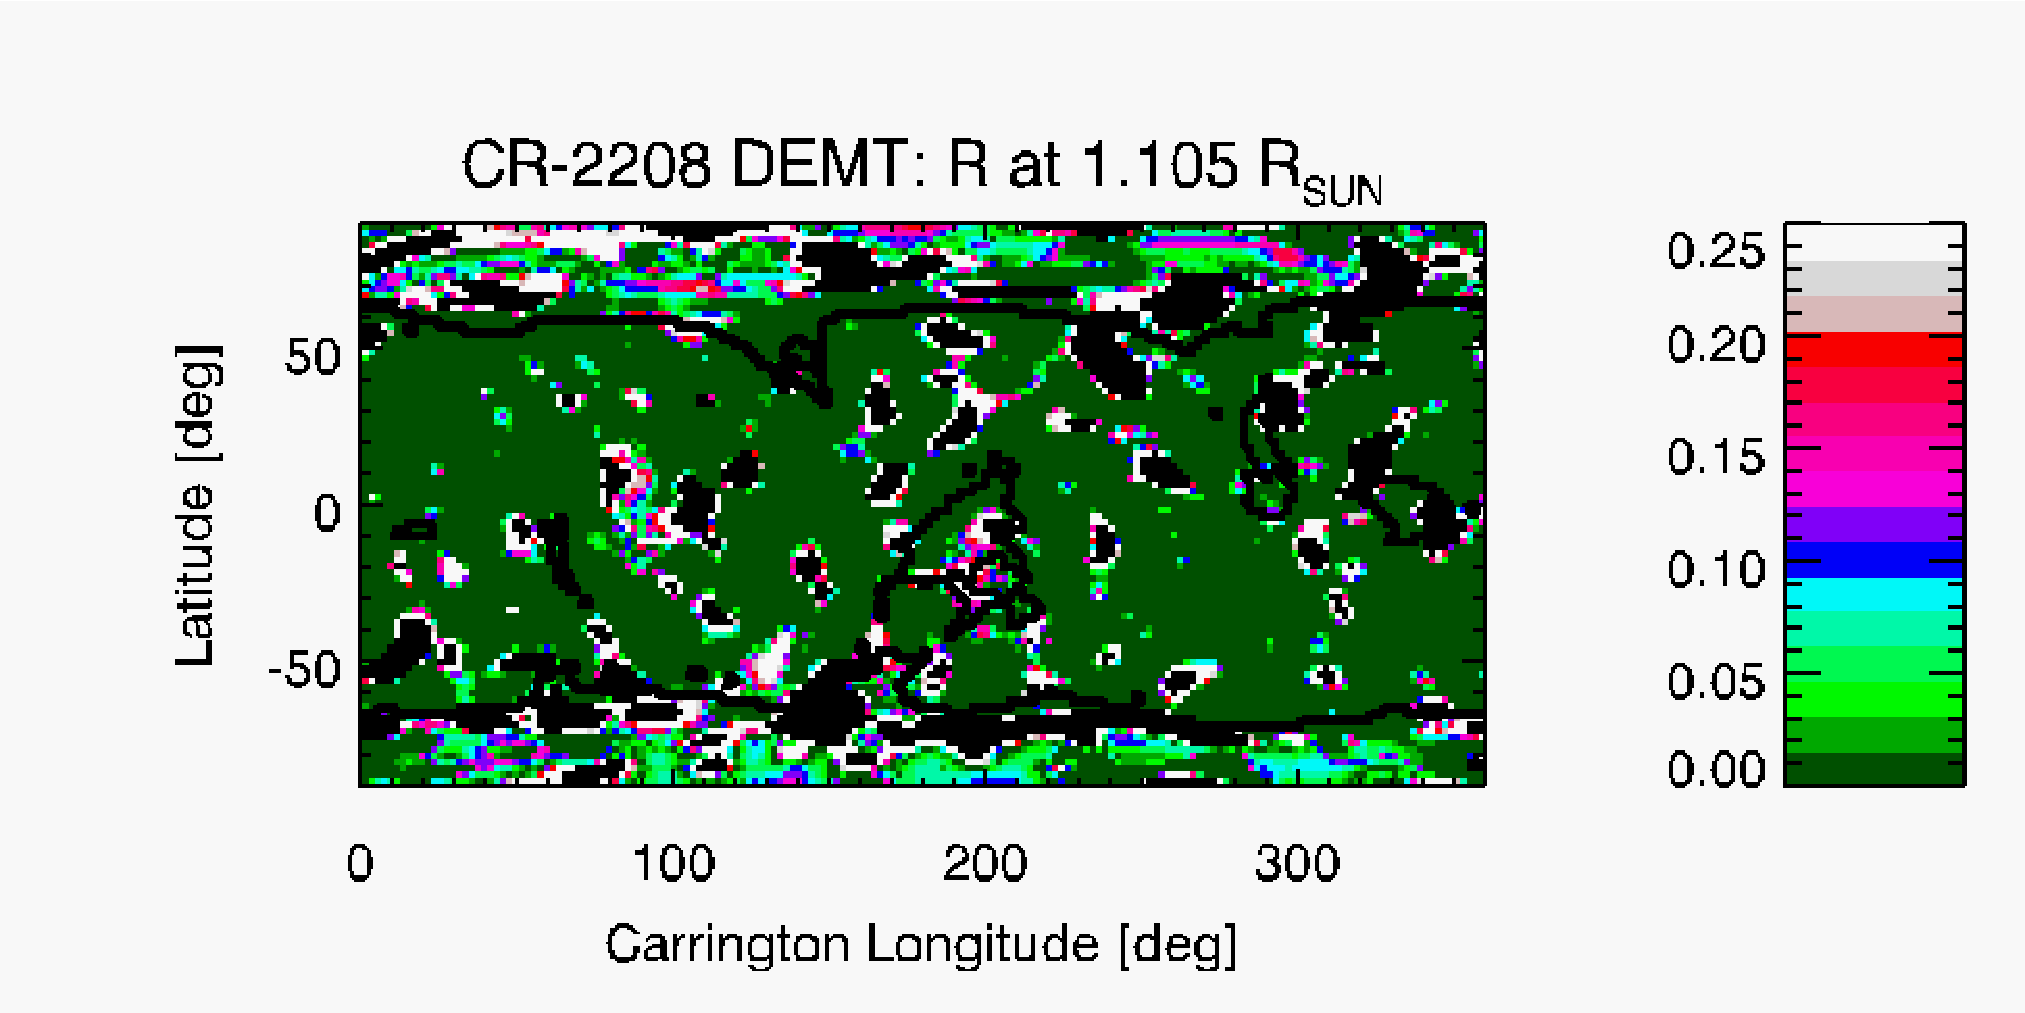
\includegraphics[width=0.495\textwidth]{figs/map_R_CR2208_DEMT-AIA_H1_L522_r3d_1105_Rsun.pdf}
\caption{{Carrington maps of the measure $R$ defined by Equation (\ref{R}), for CR-2082 (left panels) and CR-2208 (right panels), at heights $1.025$, $1.065$ and $1.105\,\mrsun$, from top to bottom}. }
\label{carmaps_R_2082_2208}
\end{center}
\end{figure}

{To characterize the DEMT results in different magnetic structures, we traced} $\sqravgN$ and $\Tm$ along the magnetic field lines of the AWSoM model. For both rotations, all field lines that meet the criteria listed in Section \ref{trace} were selected. For each field line, the data points of electron density and electron mean temperature as a function of height were fitted to the Equations \ref{Nfit} and \ref{Tfit}. {As a result, the electron density $N_0(r=1.0\,\mrsun)$ and scale height $\lN$ were computed for each leg, as well as the temperature gradient $\dr\Tm$, and the height-averaged (along the leg) {electron temperature} $\aTm$.}

\begin{figure}[h!]
\begin{center}
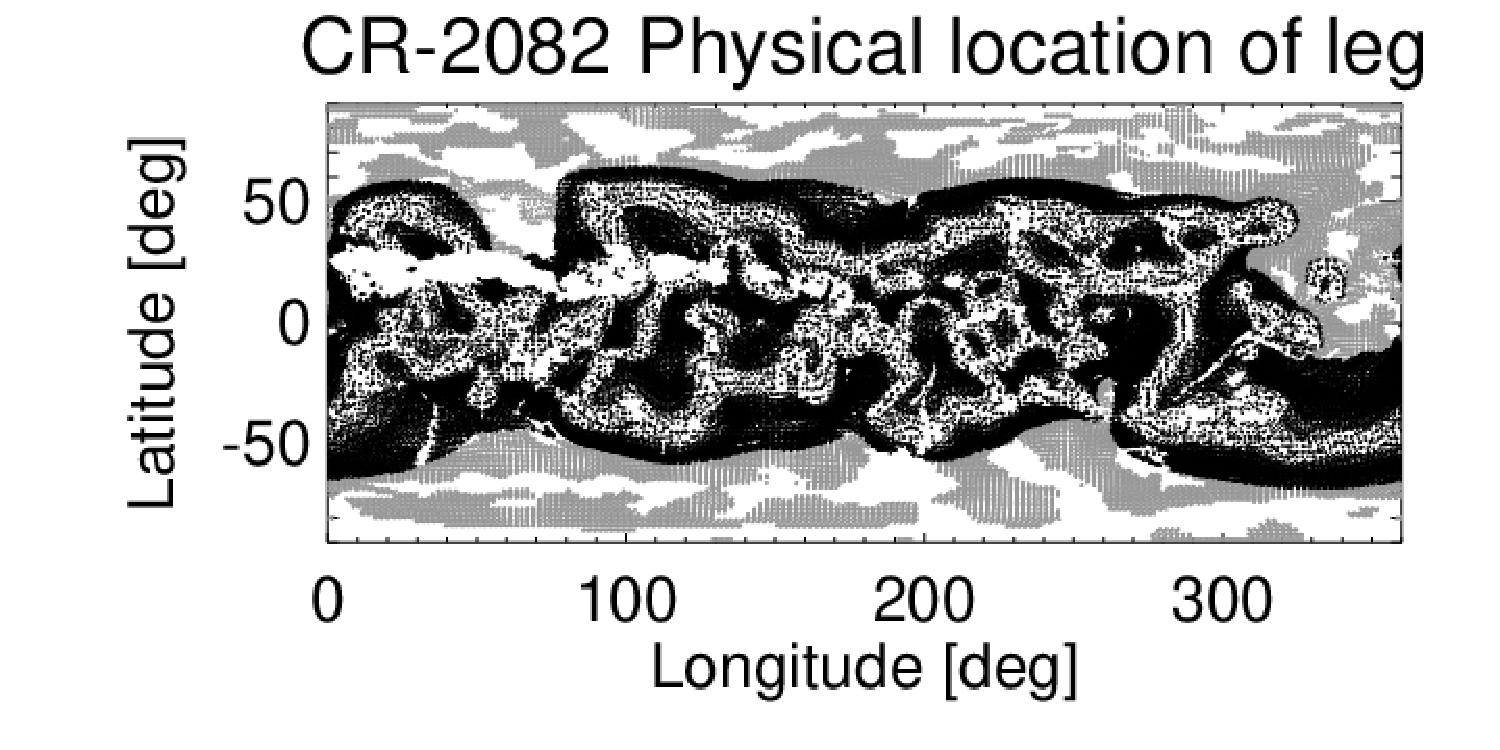
\includegraphics[width=0.495\textwidth,clip=]{figs/Grispoint_2082_demt_paper_test_Rpoint-map.pdf}
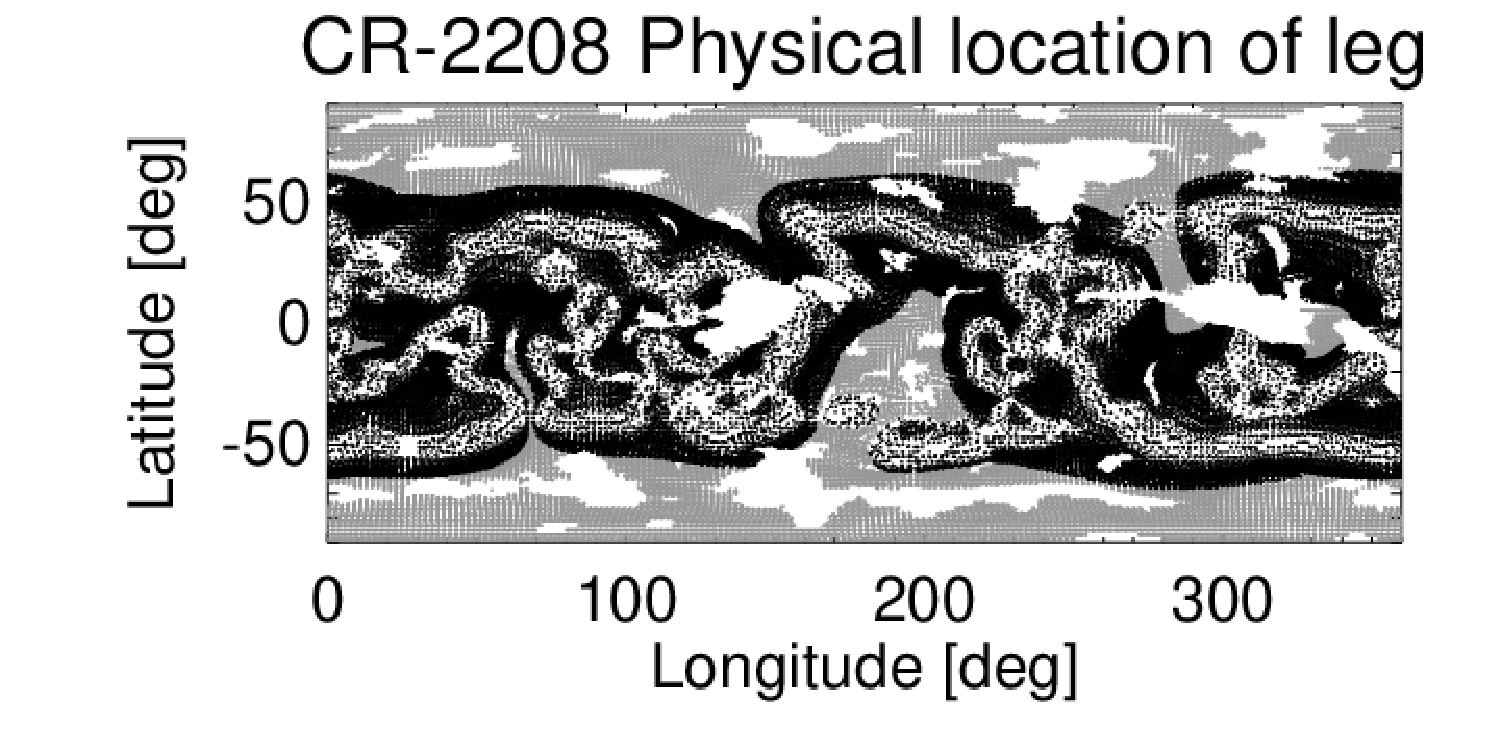
\includegraphics[width=0.495\textwidth,clip=]{figs/Grispoint_2208_demt_paper_test_Rpoint-map.pdf}
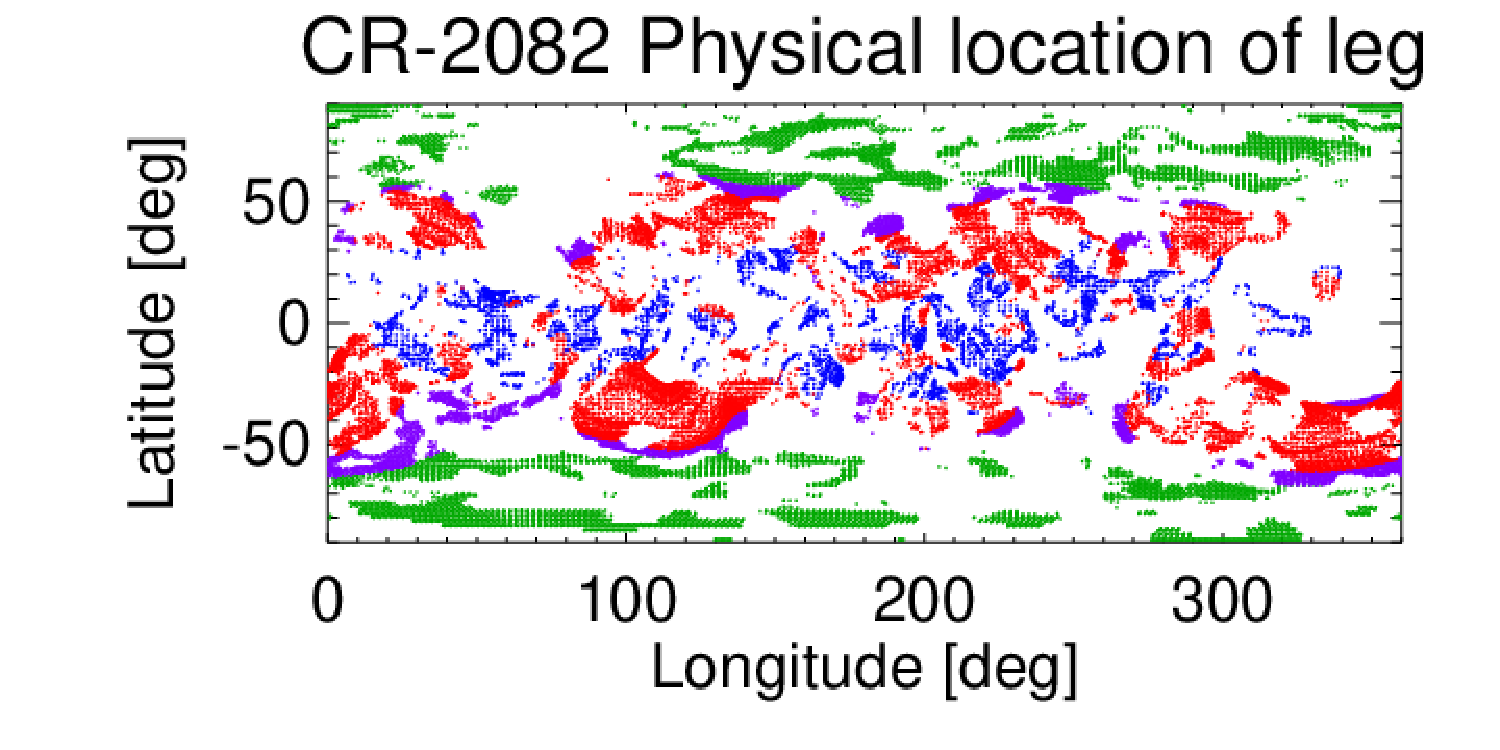
\includegraphics[width=0.495\textwidth,clip=]{figs/Highpoint_2082_demt_paper_cr2082_full_Rpoint-map.pdf}
%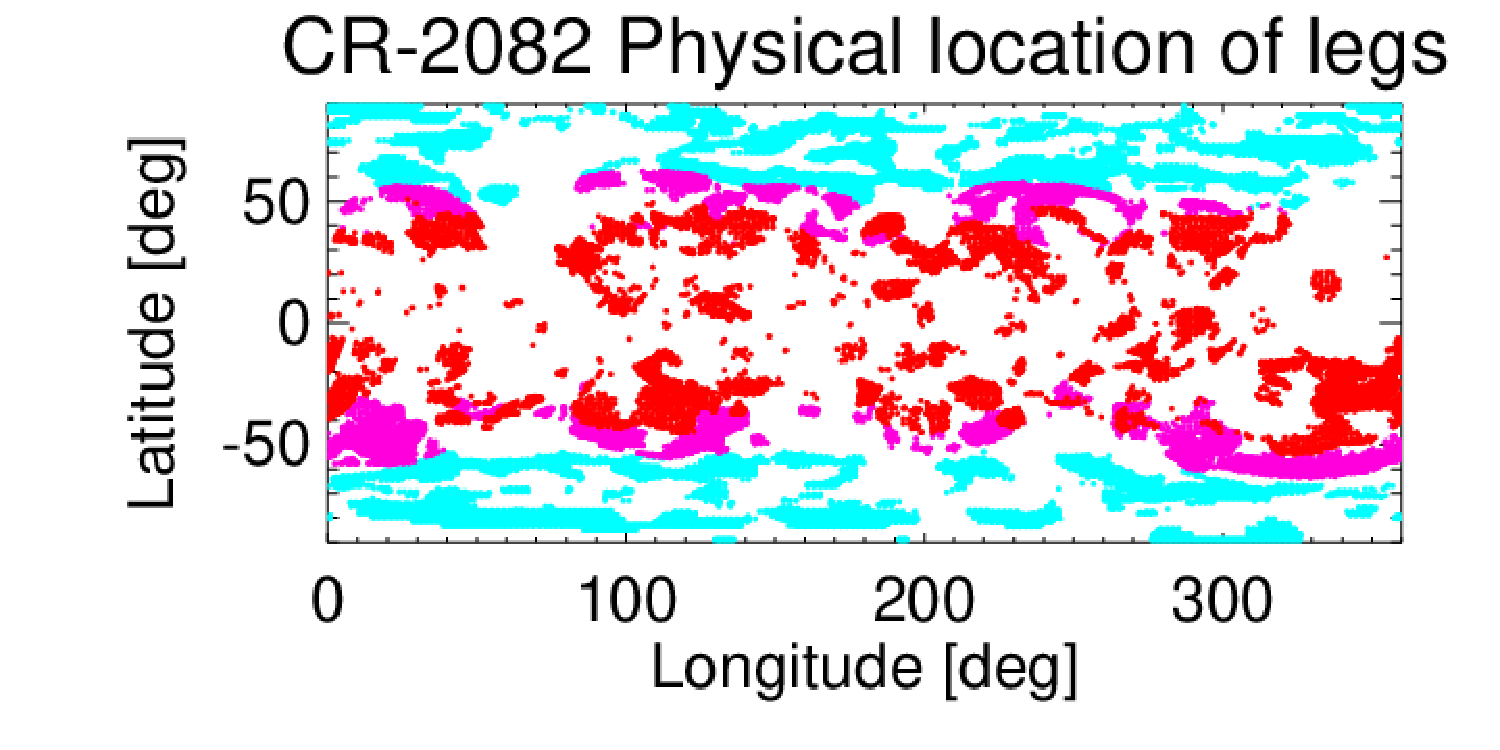
\includegraphics[width=0.495\textwidth,clip=]{figs/Highpoint_2082_demt_paper_cr2082_up_Rpoint-map.eps}
%\includegraphics[width=0.495\textwidth,clip=]{Highpoint_2082_awsom_paper_Rpoint-map.eps}
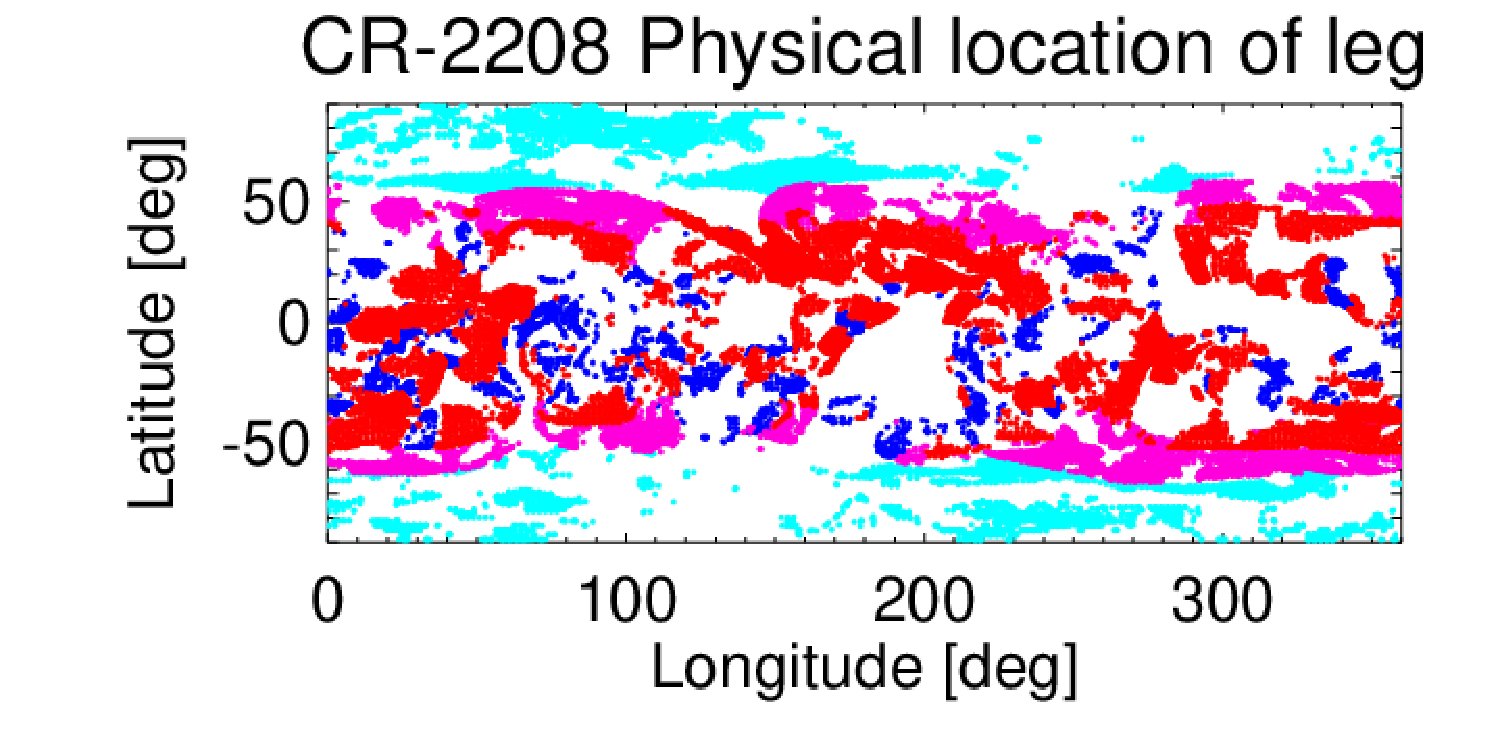
\includegraphics[width=0.495\textwidth,clip=]{figs/Highpoint_2208_demt_paper_cr2208_full_Rpoint-map.pdf}
%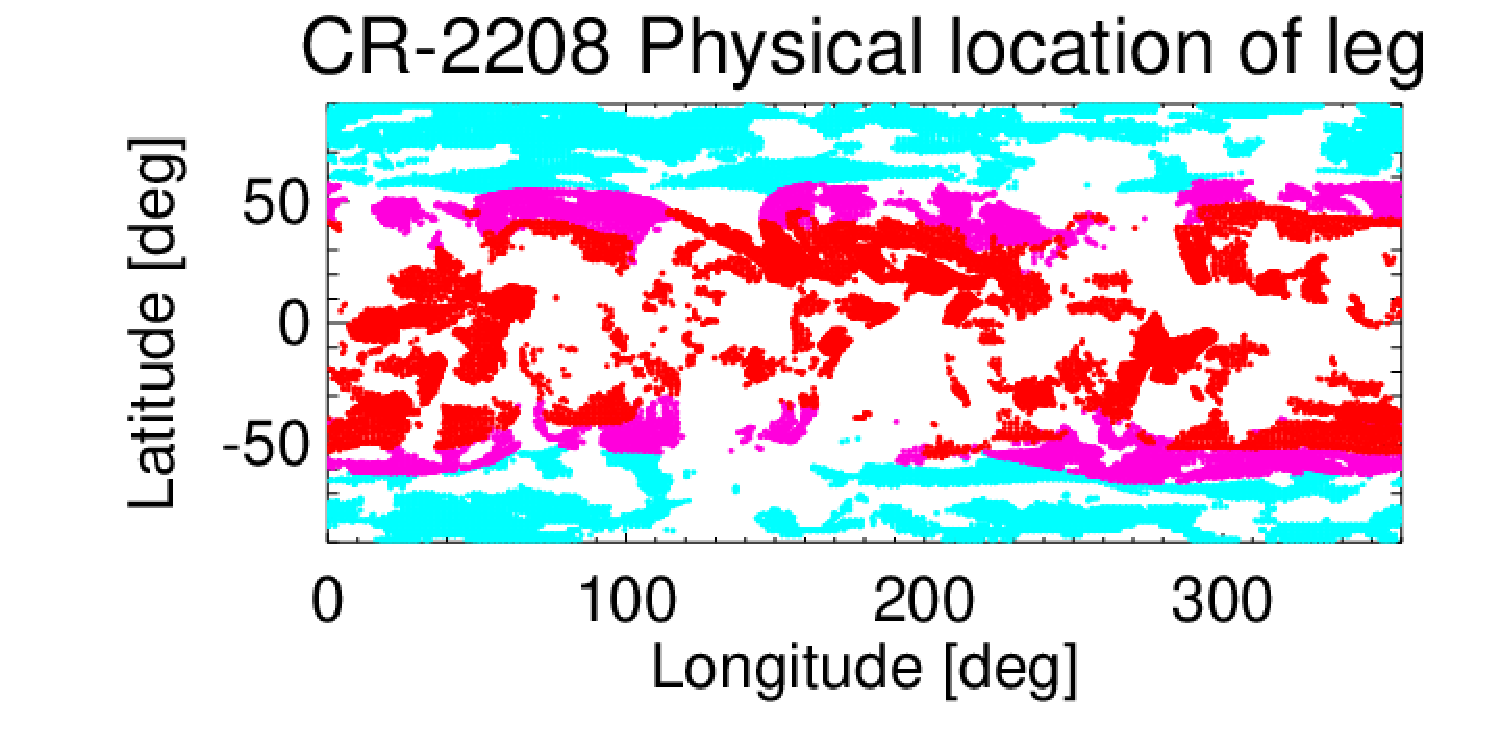
\includegraphics[width=0.495\textwidth,clip=]{figs/Highpoint_2208_demt_paper_cr2208_up_Rpoint-map.eps}
%\includegraphics[width=0.495\textwidth,clip=]{Highpoint_2208_awsom_paper_Rpoint-map.eps}
\caption{\emph{Top panels:} {latitude-longitude location at heliocentric height $r=1.105\,\mrsun$ of all open (grey color) and closed (black color) traced field line legs for which criterion (i) of Section \ref{trace} is met, for both CR2082 (left) and CR2208 (right). \emph{Bottom panels}: latitude-longitude location of the subset for which also both criteria (ii) and (iii) of Section \ref{trace} are met. {The location of} type 0, I, II and III legs {is shown} in blue, red, {magenta and cyan} color, respectively.}}
\label{rpoint_demt}
\end{center}
\end{figure}

{For both target rotations, the top panels of Figure \ref{rpoint_demt} show the latitude-longitude location (at heliocentric height $r=1.105\,\mrsun$) of all traced field line legs for which criterion (i) of Section \ref{trace} is met. Open legs are indicated in gray color and closed ones in black color. For each leg, the fits to tomografic temperature and density were applied, as given by Equations (\ref{Nfit})-(\ref{Tfit}). Considering the DEMT data points and the resulting fits along each leg, the bottom panels of Figure \ref{rpoint_demt} show the latitude-longitude location of the subset for which also both criteria (ii) and (iii) of Section \ref{trace} are met. Using a four-color code, type 0, I, II and III legs are shown in blue, red, {magenta and cyan} color, respectively.} Of the 48000 legs selected for CR-2082, 21\% are type 0, 31\% are type I, 22\% are type II and 26\% type III. On the other hand, of the 57000 legs selected for CR-2208, 9\% are type 0, 36\% are type I, 26\% are type II and 29\% type III. \notebyalbert{Luego de des-ralear, las piernas seleccionadas en Figura 4 eran del orden de 100 mil, para  ambas rotaciones. Algo no está consistente aquí.}\diego{Statloop 6 alturas noda algo asi como 150k piernas, algunas no se trazan (entre 30 y 40k) lo cual nos deja aprox 110k. SUpongo que te quedaste con ese numero. Pero elimino los cuasi isotermicos, perdemos 30k en el streamer y 10k en CH. Luego hacemos una seleccion qie involucra footpoints y ahi perdemos lo que falta! Es decir, el numero del draft ya es des-raleado.}

{Type 0 (small down) legs mainly populate the equatorial latitudes. This kind of structure was originally found by \citet{huang_2012}, and their existence was shown to be anti-correlated with the solar activity level {around the solar minimum between SCs 24 and 25} by \citet{nuevo_2013}. Later on, \citet{lloveras_2017} showed {that} equatorial down loops in streamers were also to be found in the deep minimum between SCs {23 and 24}. Here, we verify the existence of this type of structure for the two target rotations. The relatively smaller population of down loops seen in CR-2208, as compared to CR-2082, is consistent with the aforementioned results by \citet{nuevo_2013}. Type I (small up) mainly populate the mid-latitudes, while type II (large up) legs are mostly very large trans-equatorial field lines forming the envelope of the streamer belt. Finally, type III (open) legs populate of course the CHs.}

\begin{figure}[h!]
\begin{center}
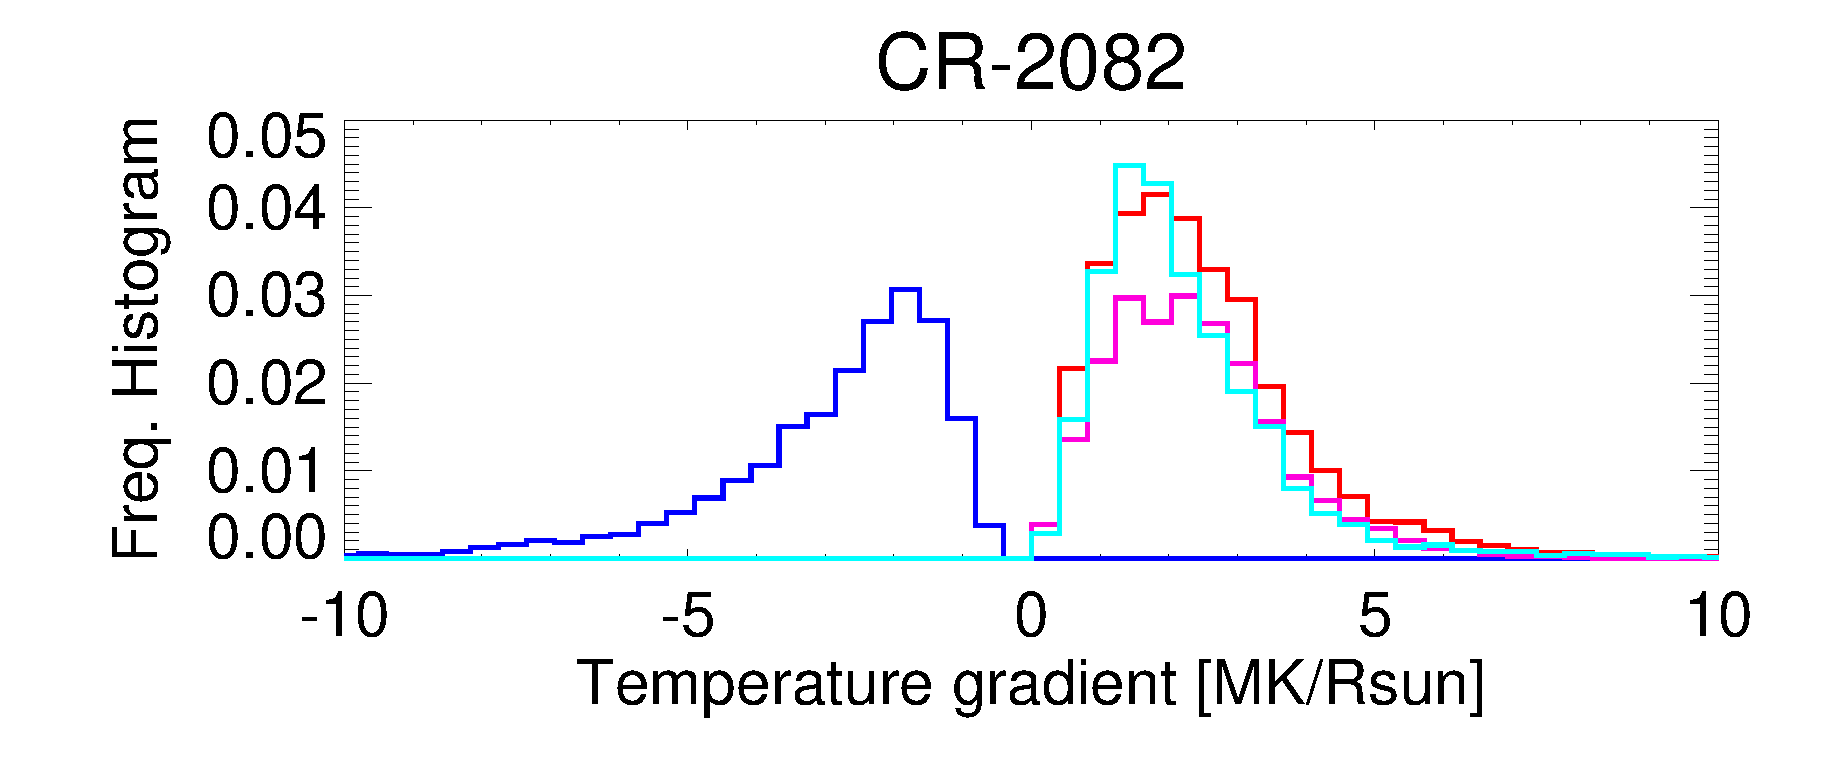
\includegraphics[width=0.495\textwidth,height=0.25\textwidth,clip=]{figs/histo_cr2082_fulltriple_gradt.eps}
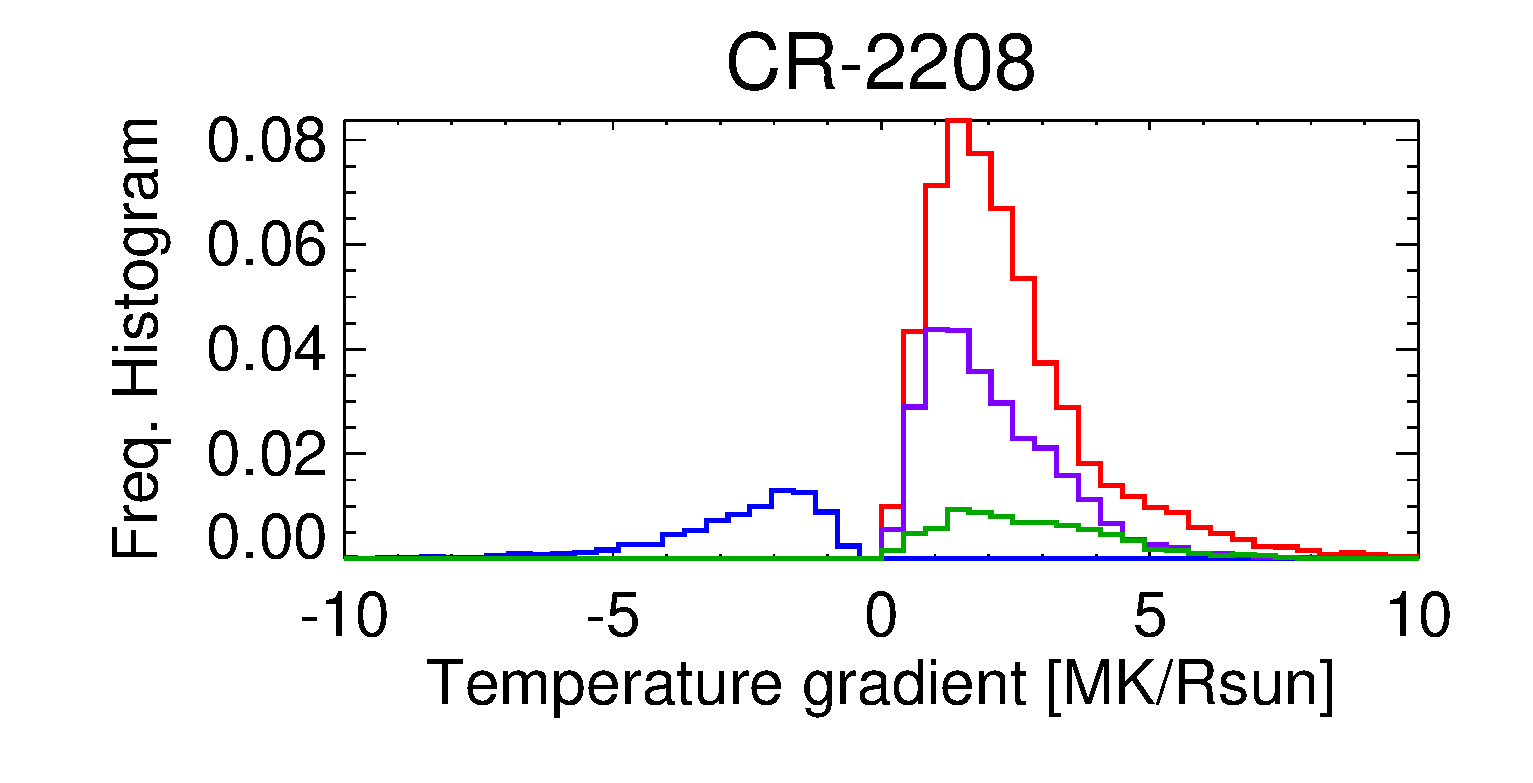
\includegraphics[width=0.495\textwidth,height=0.25\textwidth,clip=]{figs/histo_cr2208_fulltriple_gradt.eps}
\caption{Frequency histograms of the temperature radial gradient for {the four types of legs} in Figure \ref{rpoint_demt} (using the same color code) for CR-2082 (left panel) and CR-2208 (right panel).}
\label{gradt_demt}
\end{center}
\end{figure} 

Figure \ref{gradt_demt} shows frequency histograms (normalized to the total amount of selected field lines ) of the temperature radial gradient ($\dr\Tm$) for legs of type 0, I, II and III. The lack of population around values close to zero is due to the requirement $|\rhoTr| > 0.5$ which discards quasi-isothermal legs. For both rotations, {the median value of the temperature radial gradient is ${\rm Md}\left(\dr\Tm\right) \approx -2.5$, $+2.3$ and $+2.4\,\MK/\mrsun$} for legs of type 0, I and II, respectively.

{The notable difference between both rotations is the characteristic {value ${\rm Md}\left(\dr\Tm\right)\approx +4.5\,\MK/\mrsun$} for legs of type III for CR-2208. This is related to the much larger $R$ score for the DEMT results along CH legs for CR-2208. In this case, DEMT performs poorly in modeling a LDEM that predicts the tomographic FBEs with reasonable accuracy. Indeed, visual inspection of the DEMT temperature maps for CR-2208 in Figure \ref{momento2}, {reveals that in most of the CH region the result for $\Tm$ below height $1.105\,\mrsun$ is quite uniform and artificially low}. As it turns out, around and above height this height the score $R$ is lower and the temperature results are more reliable. As a result, the temperature gradient along these legs is artificially larger, with the linear fit trying to simultaneously fit the artificially low values of $\Tm$ at lower heights. In general, the DEMT results in the CH region based on AIA data are thus much less reliable than in the rest of the analysis. We will return to this point in the conclusion section.}

\begin{figure}[h!]
\begin{center}
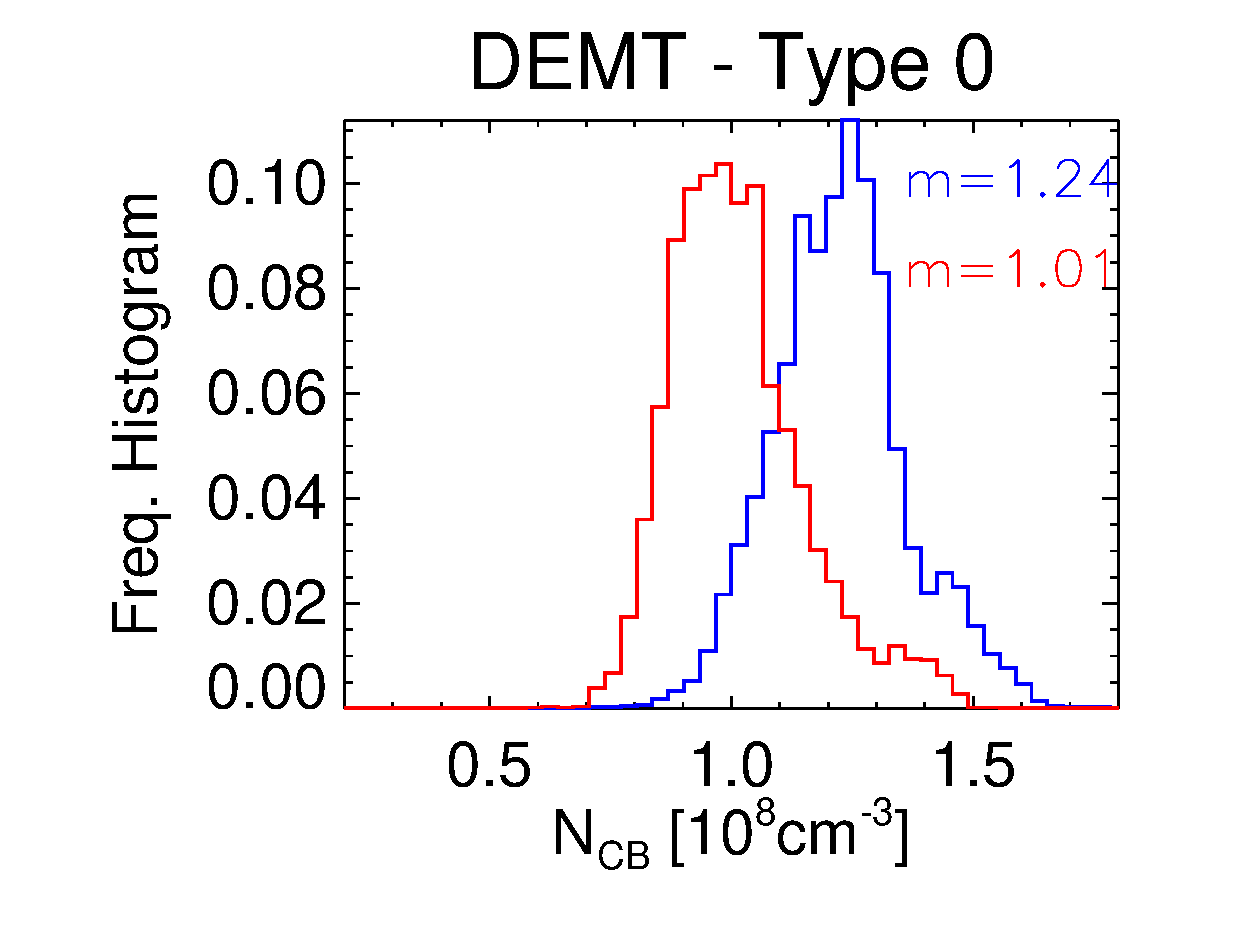
\includegraphics[width=0.31\textwidth,clip=]{figs/histo_2082_2208_fulldemt_streamer_down_ne_1055.eps}
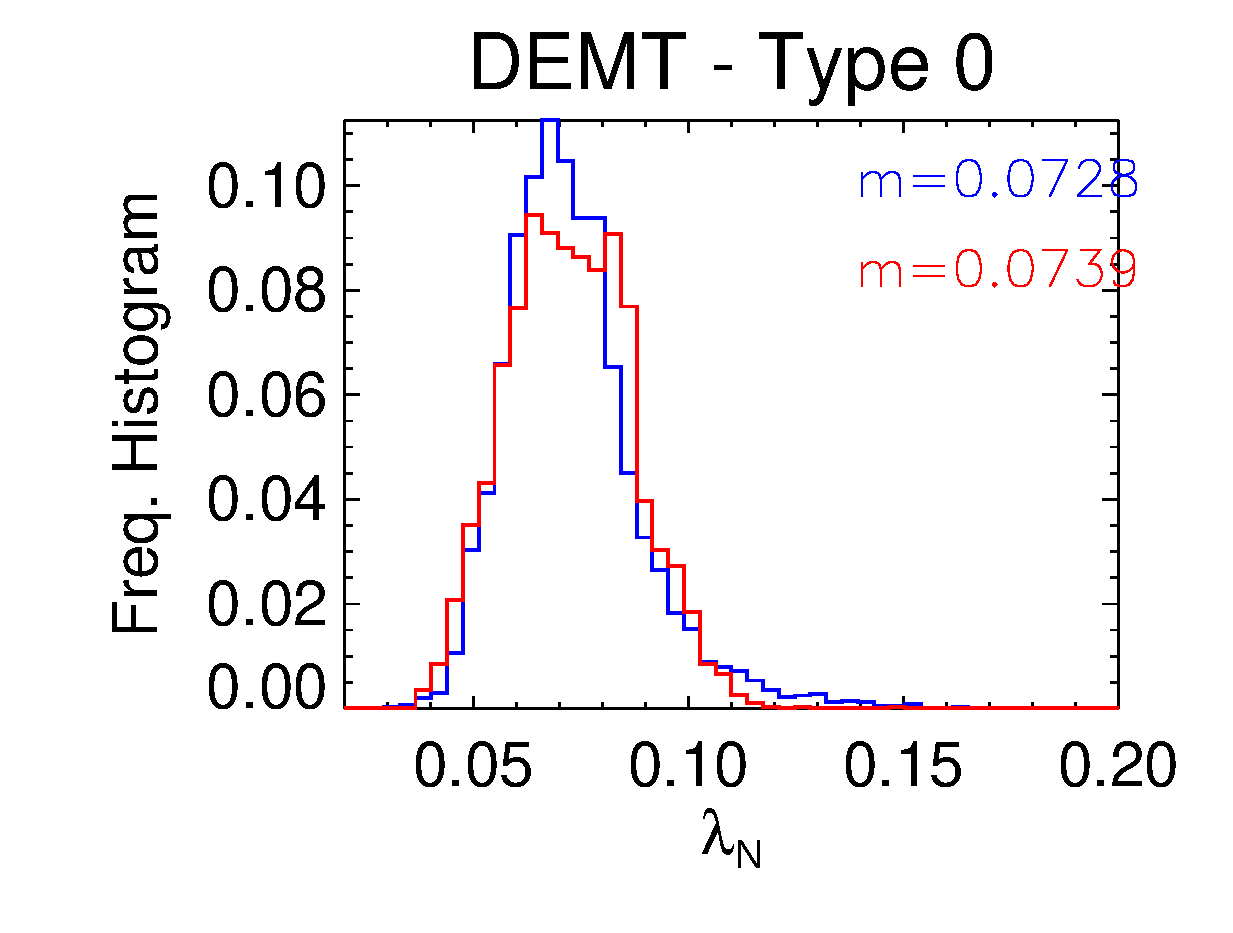
\includegraphics[width=0.31\textwidth,clip=]{figs/histo_2082_2208_fulldemt_streamer_down_lambda_n.eps}
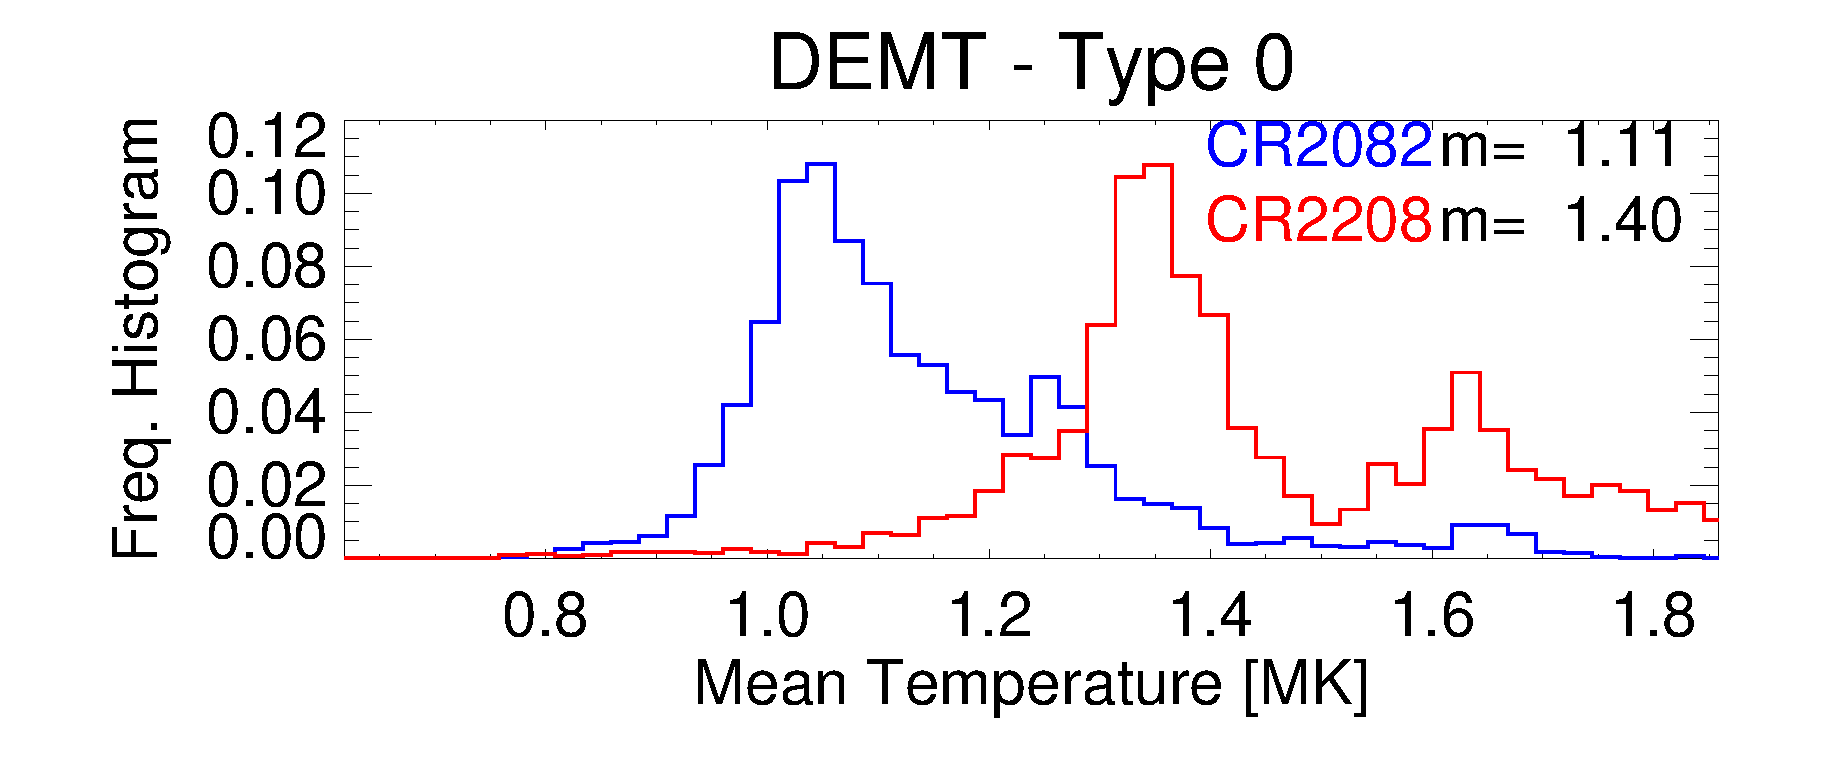
\includegraphics[width=0.31\textwidth,clip=]{figs/histo_2082_2208_fulldemt_streamer_down_Tm.eps}
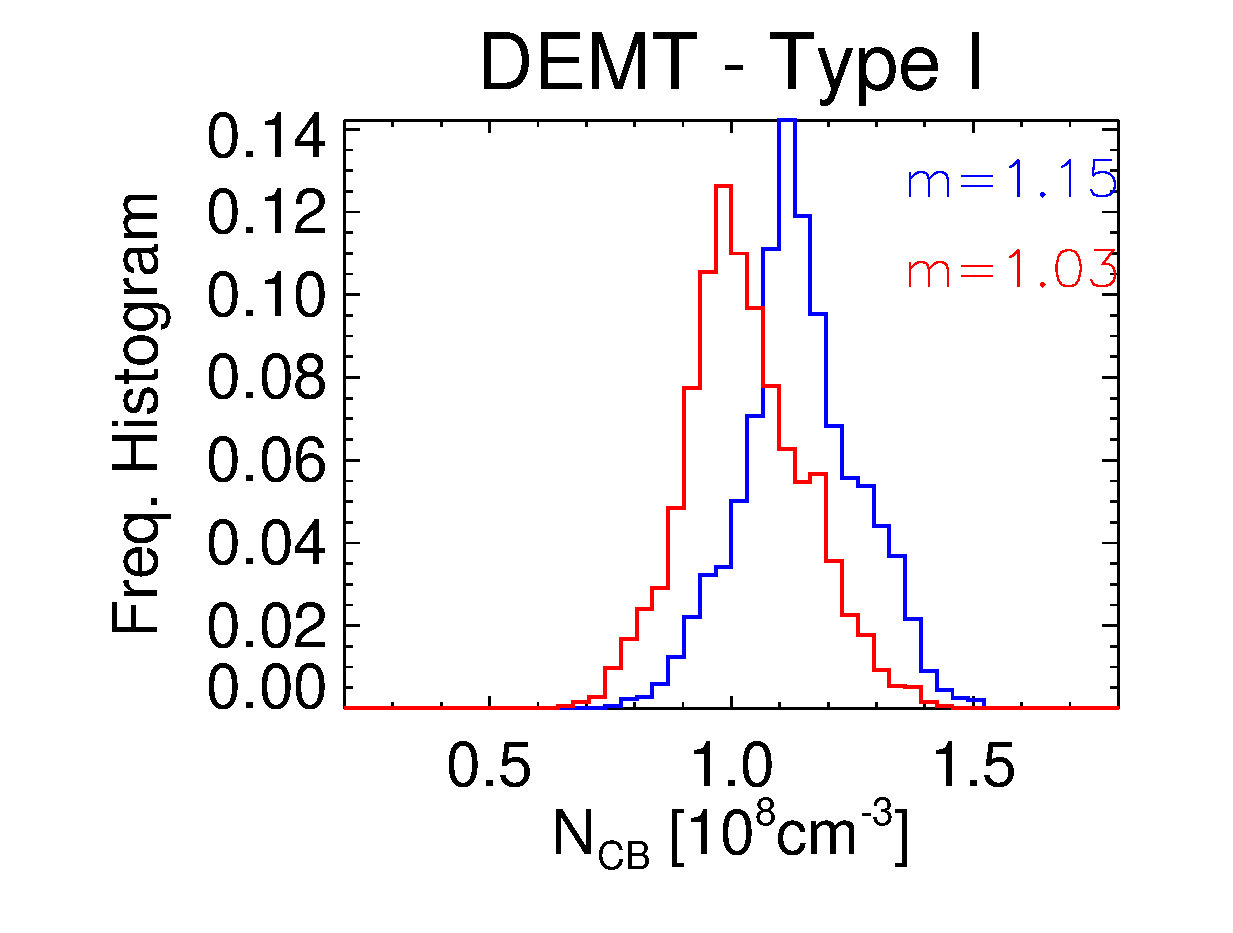
\includegraphics[width=0.31\textwidth,clip=]{figs/histo_2082_2208_fulldemt_streamer_up_ne_1055.eps}
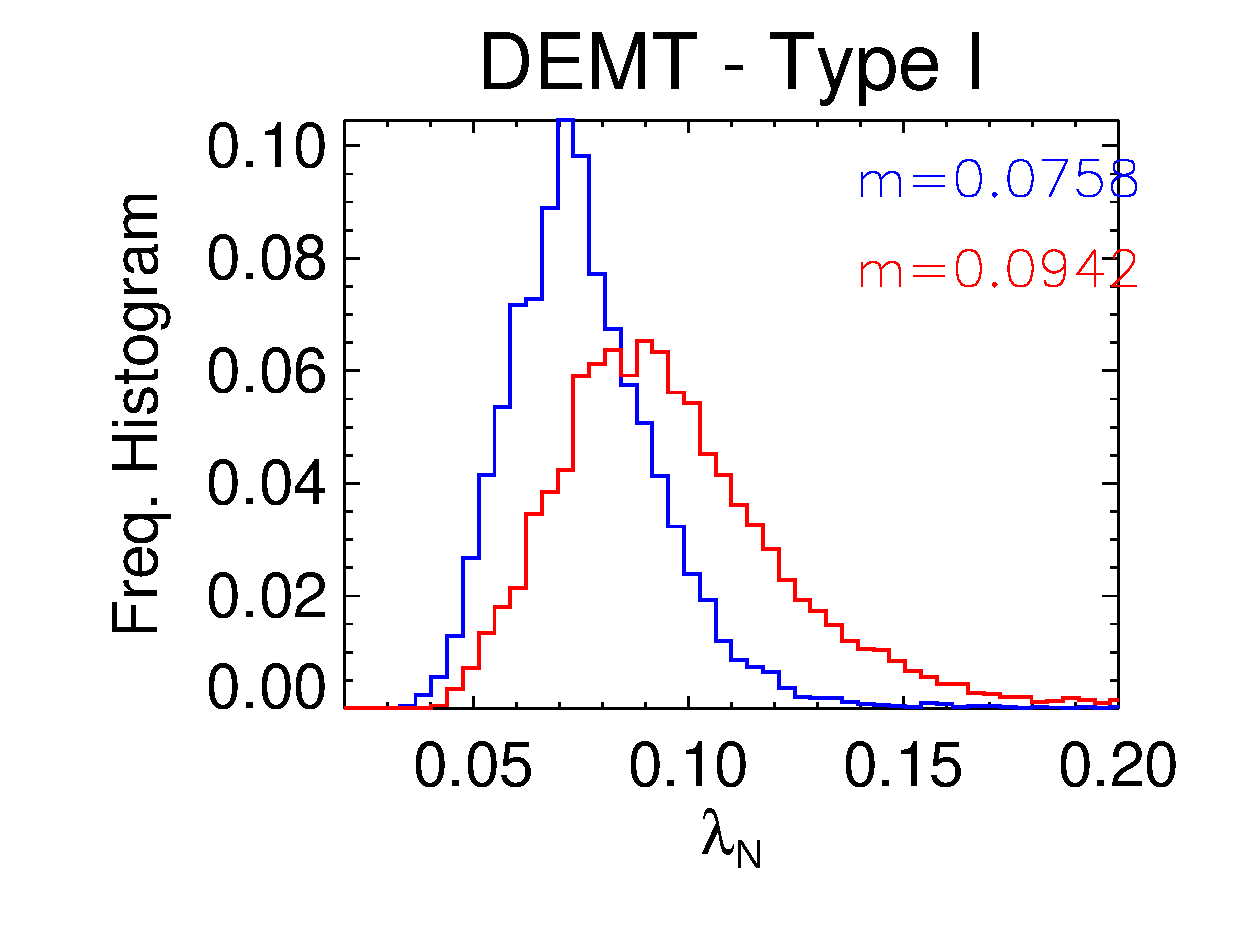
\includegraphics[width=0.31\textwidth,clip=]{figs/histo_2082_2208_fulldemt_streamer_up_lambda_n.eps}
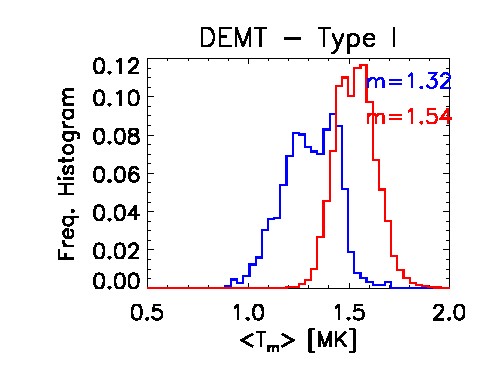
\includegraphics[width=0.31\textwidth,clip=]{figs/histo_2082_2208_fulldemt_streamer_up_Tm.eps}
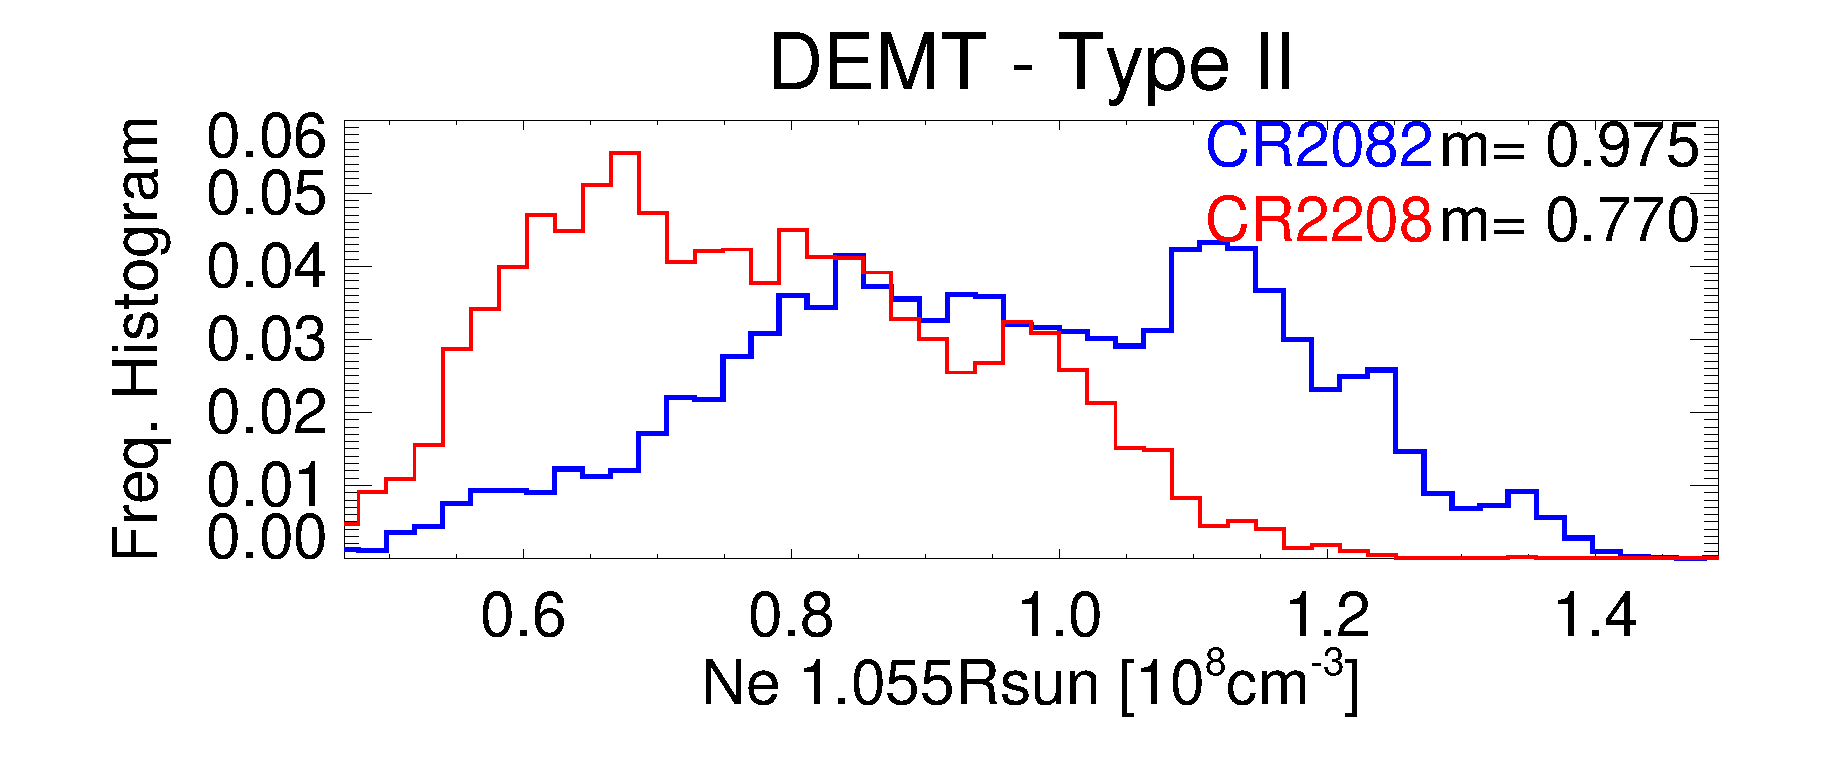
\includegraphics[width=0.31\textwidth,clip=]{figs/histo_2082_2208_fulldemt_bound_up_ne_1055.eps}
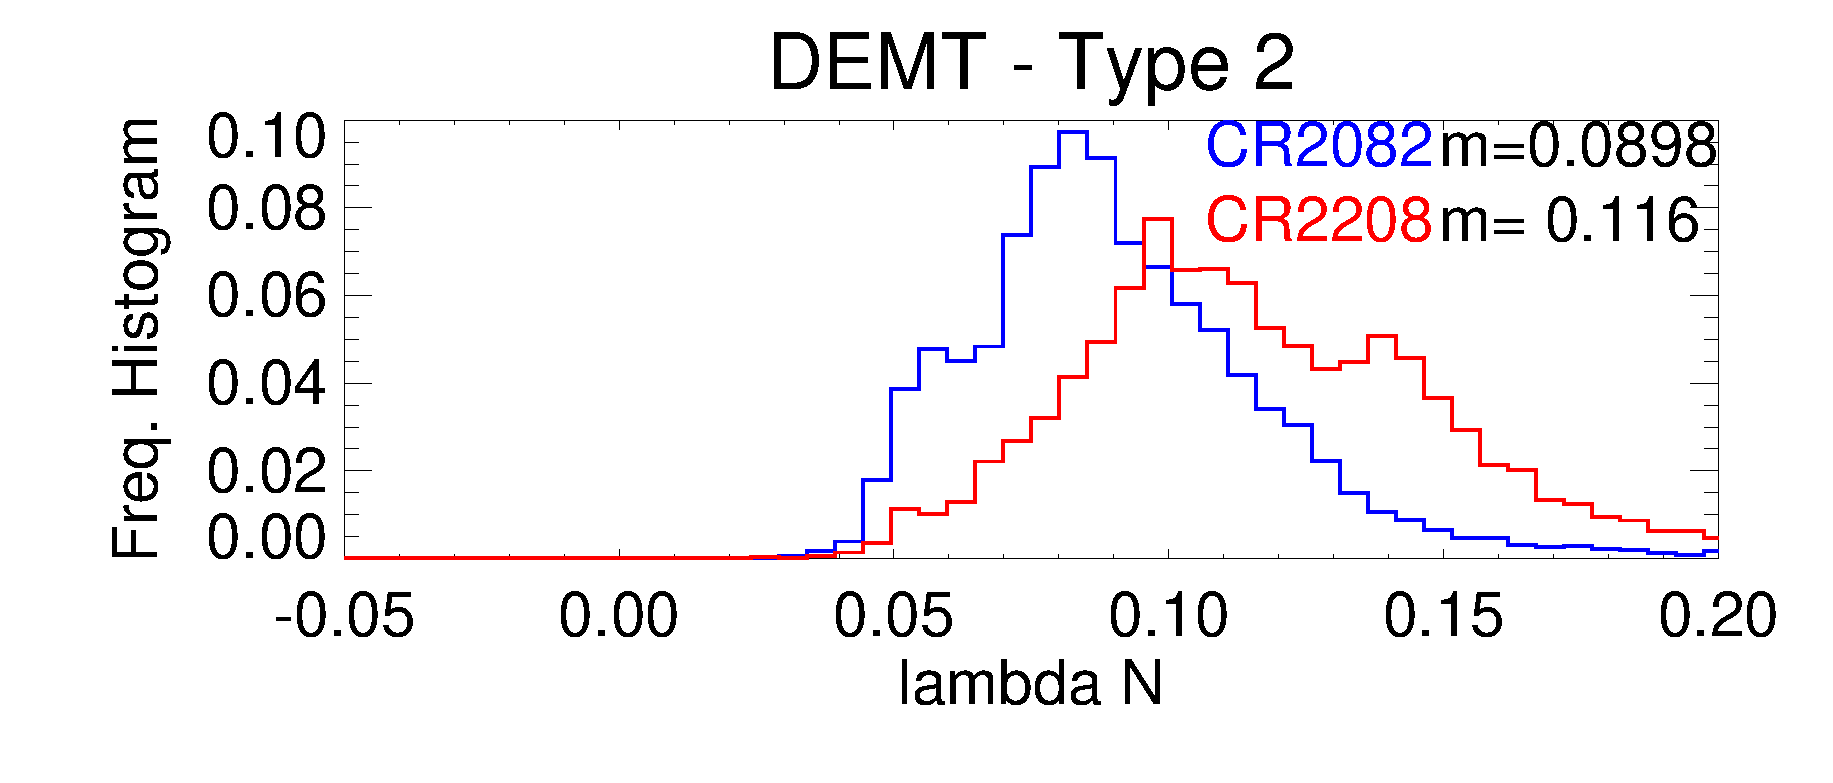
\includegraphics[width=0.31\textwidth,clip=]{figs/histo_2082_2208_fulldemt_bound_up_lambda_n.eps}
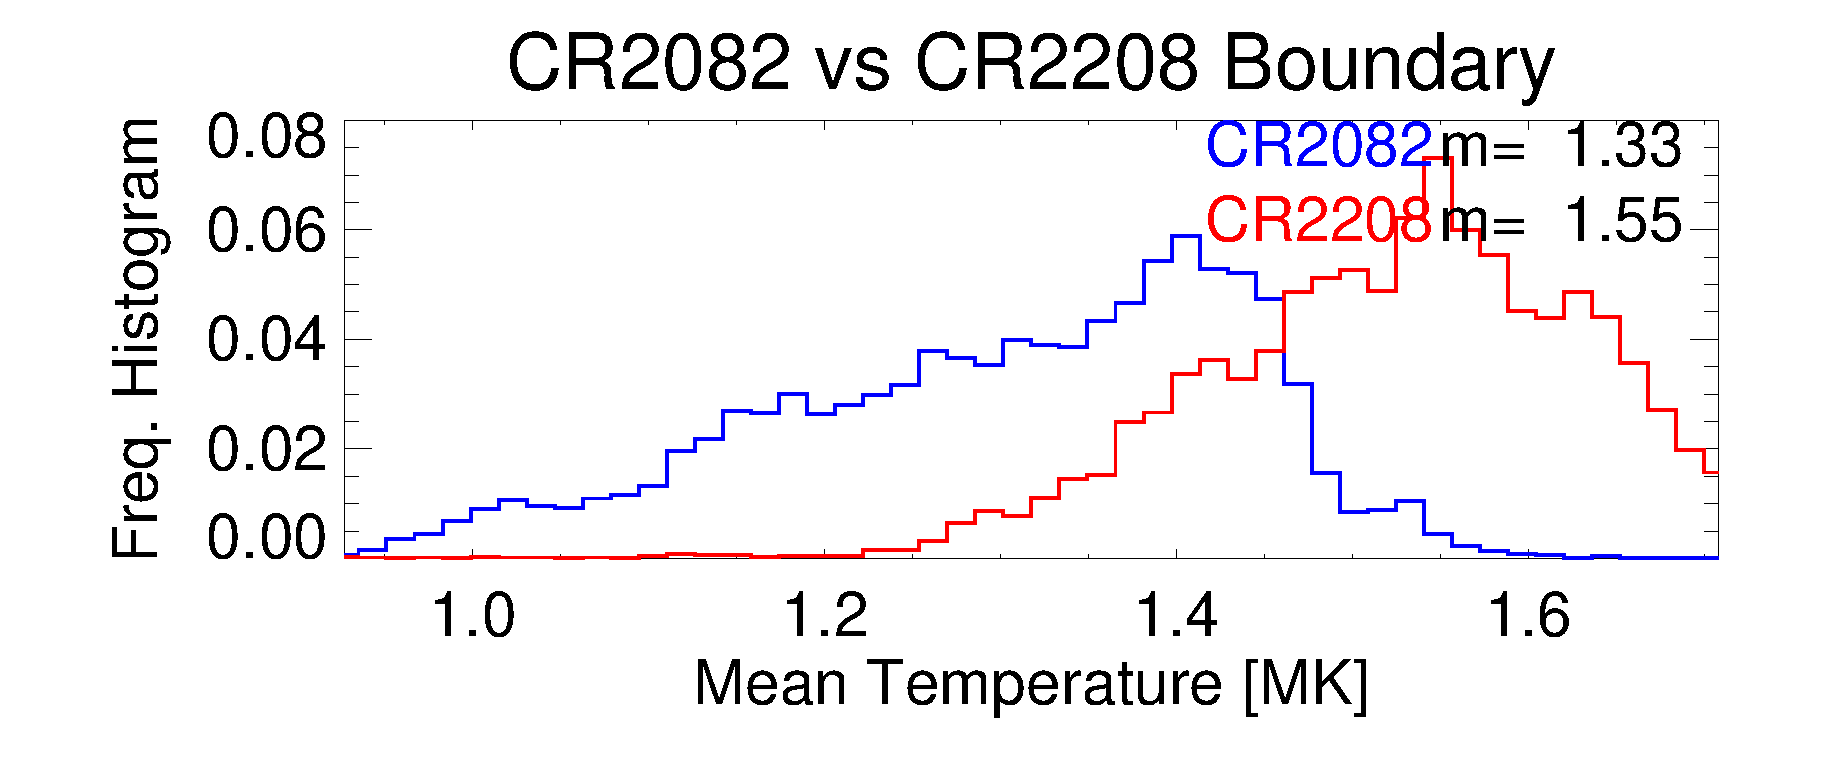
\includegraphics[width=0.31\textwidth,clip=]{figs/histo_2082_2208_fulldemt_bound_up_Tm.eps}
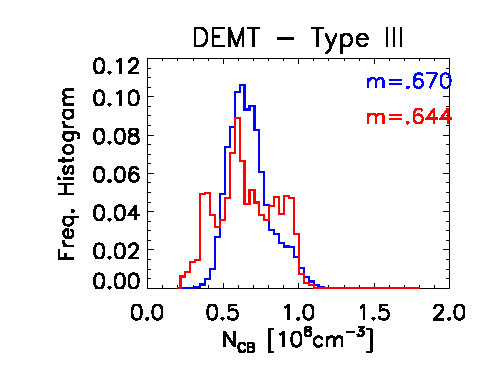
\includegraphics[width=0.31\textwidth,clip=]{figs/histo_2082_2208_fulldemt_CH_up_ne_1055.eps}
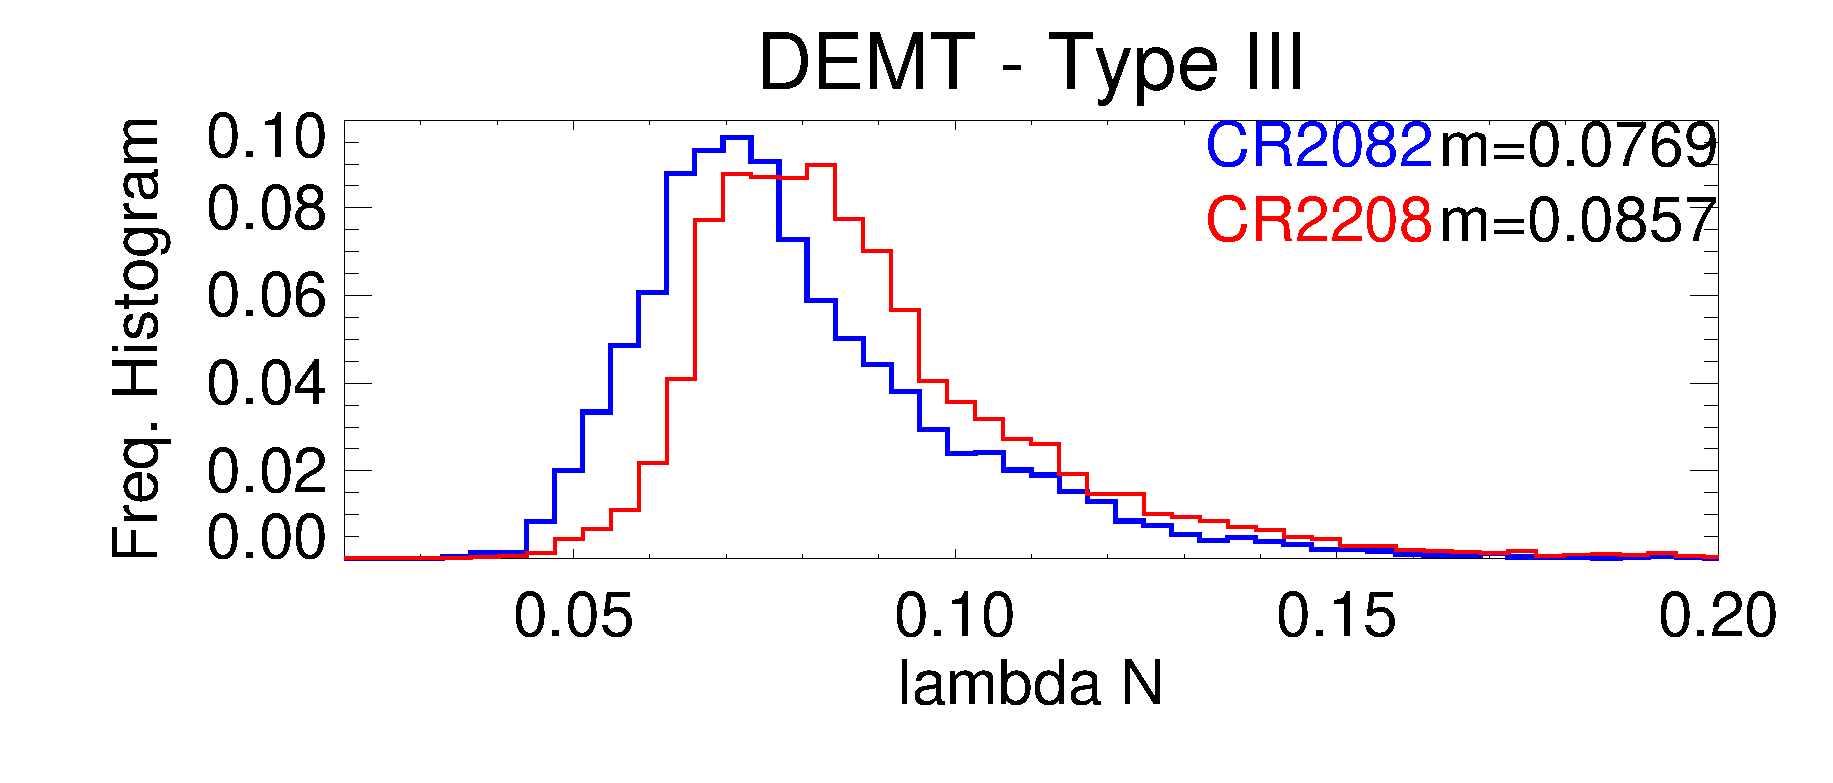
\includegraphics[width=0.31\textwidth,clip=]{figs/histo_2082_2208_fulldemt_CH_up_lambda_n.eps}
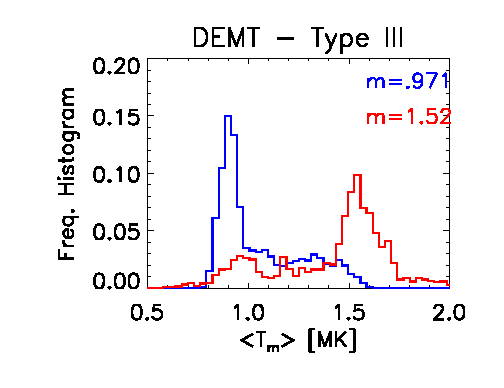
\includegraphics[width=0.31\textwidth,clip=]{figs/histo_2082_2208_fulldemt_CH_up_Tm.eps}
\caption{{Statistical distribution of {DEMT results for rotations CR-2082 (blue) and CR-2208 (red)} traced along legs of type 0, I, II and III (from top to bottom), as defined in Section \ref{trace}. From left to right: {electron density $\NCB\equiv\sqravgN(r=1.055\,\mrsun)$,} electron density scale height $\lN$, {and loop-averaged temperature $\aTm$. In each panel} the median value $m$ is indicated.} }
\label{histos_fulldemt}
\end{center}
\end{figure} 

{For both rotations, Figure \ref{histos_fulldemt} shows, in a statistical fashion, the DEMT results traced along field lines discriminated by field line type}. From top to bottom {results are shown for} type 0 to type III {field lines}{, respectively}. From left to right the panels show the statistical distribution of $\NCB \equiv \sqravgN(r=1.055)$ {(the lowest height where the AWSoM results are consistent with coronal conditions)}, $\lN$ {and} $\aTm$, {with the median value $m$ indicated in each plot}.


{Table \ref{tabla_demt} summarizes a} quantitative comparative analysis between the results of the two {target rotations}. For CR-2082 quantities are expressed as absolute values, {while} for CR-2208 they are informed {as a percentual variation} relative to the corresponding results for CR-2082. {The following major results, both concerning the structure of each rotation individually as well as their comparison, can be drawn.}

\begin{table}[h!]
\begin{tabular}{l r@{.}l@{\hskip 0.05in} r@{\hskip 0.01in} r  r@{.}l@{\hskip 0.05in} r@{\hskip 0.01in} r r@{.}l@{\hskip 0.05in} r@{\hskip 0.01in} r }
\hline
Type    & \multicolumn{4}{c}{$\med(\NCB)$}             & \multicolumn{4}{c}{$\med(\lN)$} & \multicolumn{4}{c}{$\med(\avgTe)$} \\
        & \multicolumn{4}{c}{$[10^8\,{\rm cm}^{-3}]$}  & \multicolumn{4}{c}{$[{\rm 10}^{-2}\,\mrsun]$} & \multicolumn{4}{c}{$[\MK]$} \\
\hline
0    & 1&24 &(\Mi&19\%)  &   7&1 &(\Pl&~3\%) &   1&09 &(\Pl&24\%) \\
I    & 1&15 &(\Mi&10\%)  &   7&5 &(\Pl&29\%) &   1&25 &(\Pl&24\%) \\
II   & 0&98 &(\Mi&20\%)  &   9&9 &(\Pl&19\%) &   1&36 &(\Pl&16\%) \\
III  & 0&66 &(\Mi&12\%)  &   7&7 &(\Pl&15\%) &   0&97 &(\Pl&18\%) \\
\hline          
\end{tabular}
\caption{Median value (indicated as ``Md'') of the statistical distribution of $\NCB$, $\lN$, and $\aTm$ for each coronal type of lines defined in Section \ref{trace}. For CR-2082 values are expressed in absolute terms, while for CR-2208 they are informed as a percentual variation relative to the CR-2082 value.}
\label{tabla_demt}
\end{table}

{Throughout the magnetically closed region of both rotations, type 0, I and II legs, associated to  increasingly outer regions of the equatorial streamer belt, progressively exhibit decreasing coronal base density, increasing density scale height, and increasing electron temperature. In both rotations also, type III field lines in the CHs are characterized by sub-MK temperatures, and electron density values of order $\approx 1/2$ of those observed for the type 0 and type I lines in the core of the equatorial streamer.}

{A comparison of the results between the two rotations shows that, compared to CR-2082, target rotation CR-2208 was characterized by {$\approx 10-20\%$} lower values of the electron density at the coronal base, $\approx 5-30\%$ larger values of density scale height, and {$\approx 5-25\%$} larger values of the electron temperature.} 

{To analyze the loop-integrated energy flux quantities introduced in Section \ref{trace}, we selected closed loops for which both legs have the same sign of the radial gradient of the electron temperature $\dr\Tm$.} In this way, according to the classification of both its legs, each given loop was classified as of type 0 (small down loop), I (small up loop), or II (large up loop). {For both target rotations, and for loops of type 0, I and II, Figure \ref{energia_demt} shows the frequency histogram of the loop-integrated energy flux quantities {$\phi_r$, $\phi_c$ and $\phi_h$ in blue, green and red color}, respectively.}

\begin{figure}[ht]
\begin{center}
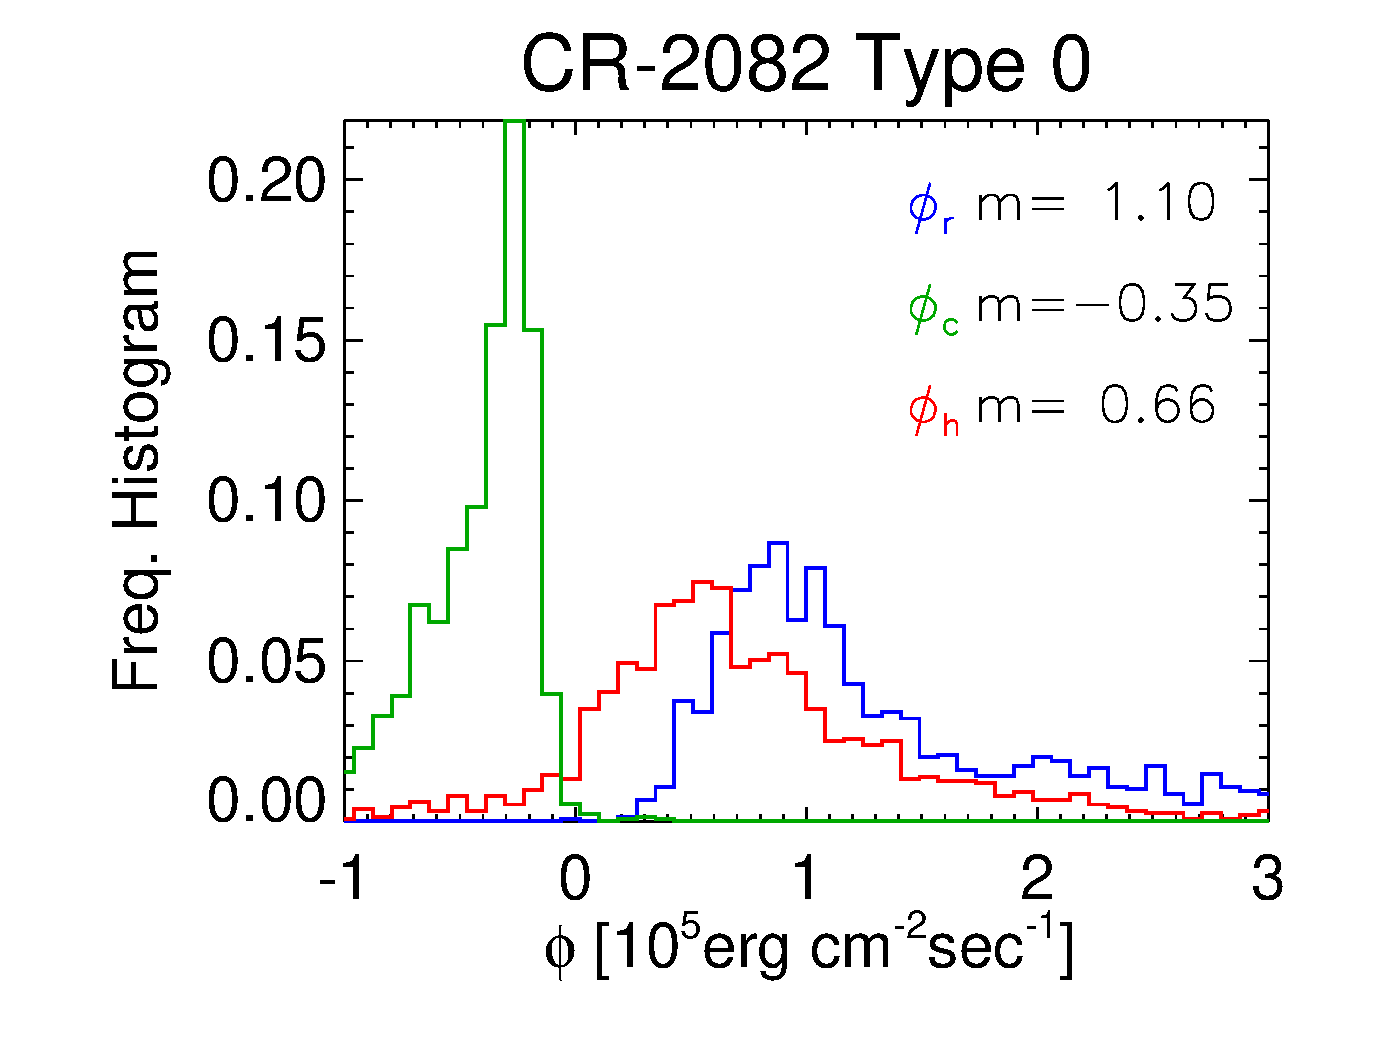
\includegraphics[width=0.495\textwidth]{figs/histocr2082_ccdownenergia.eps}
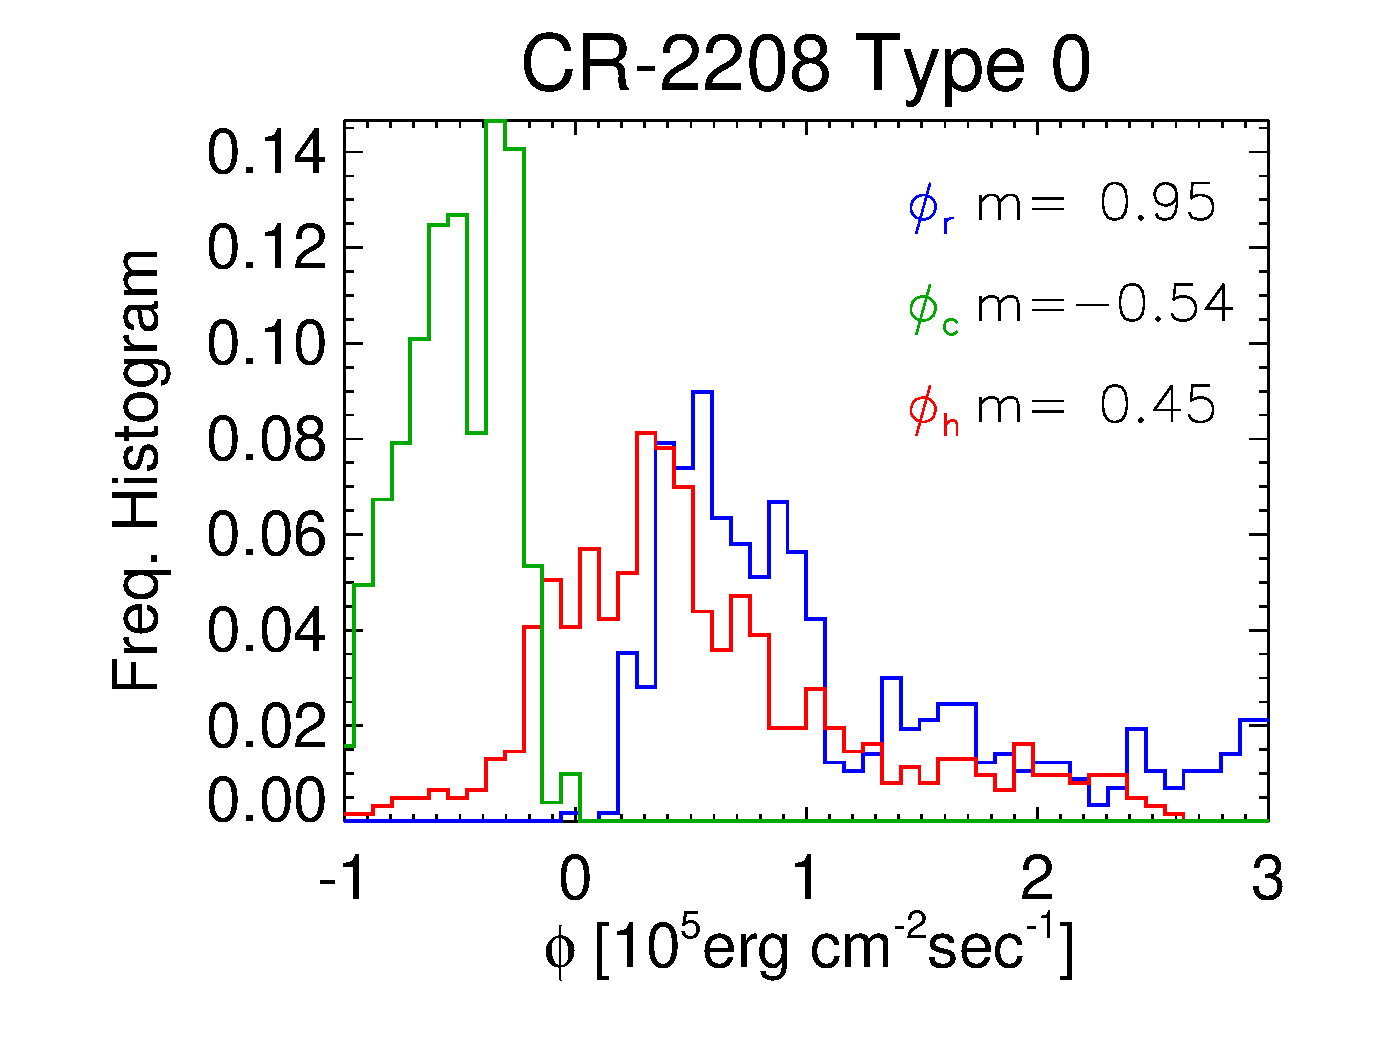
\includegraphics[width=0.495\textwidth]{figs/histocr2208_ccdownenergia.eps}
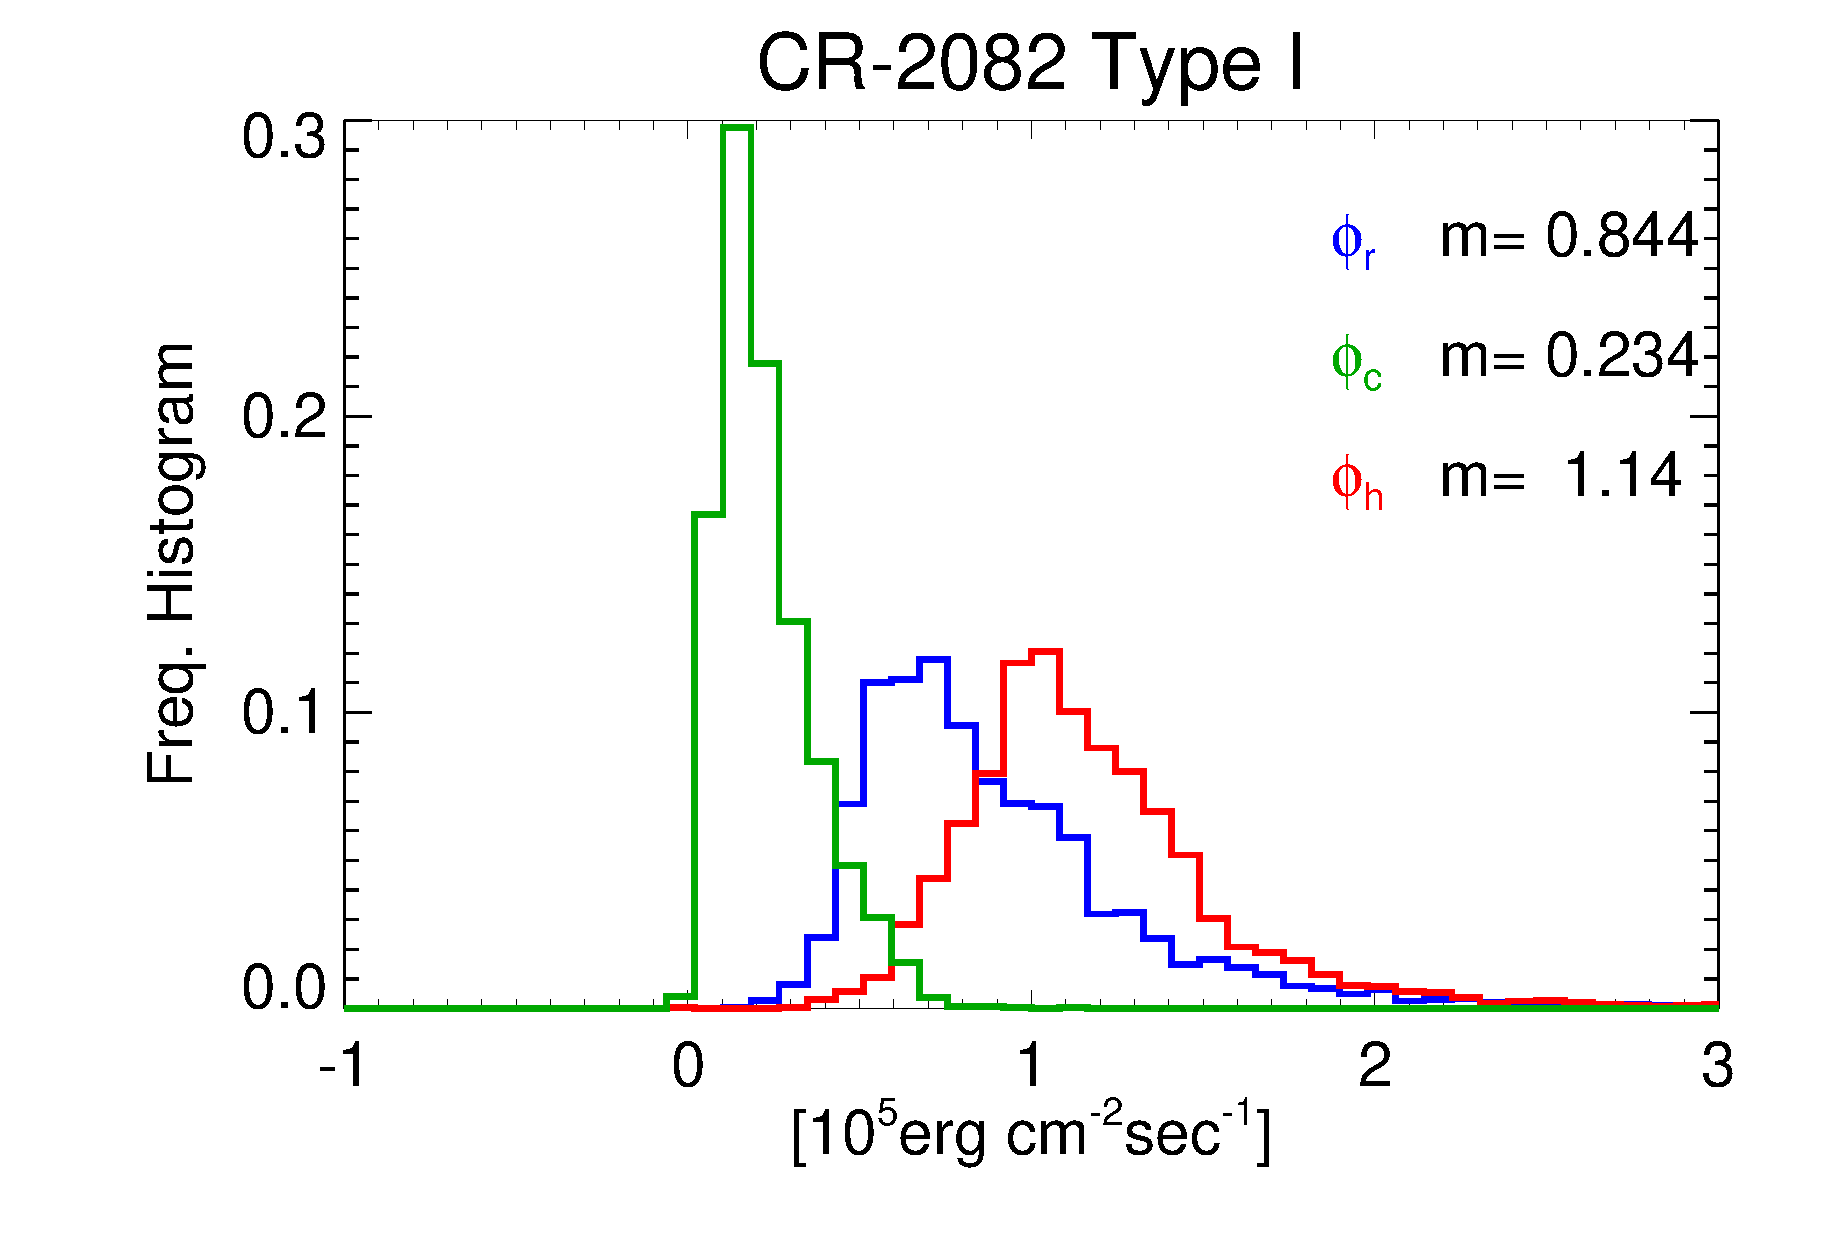
\includegraphics[width=0.495\textwidth]{figs/histocr2082_ccenergia.eps}
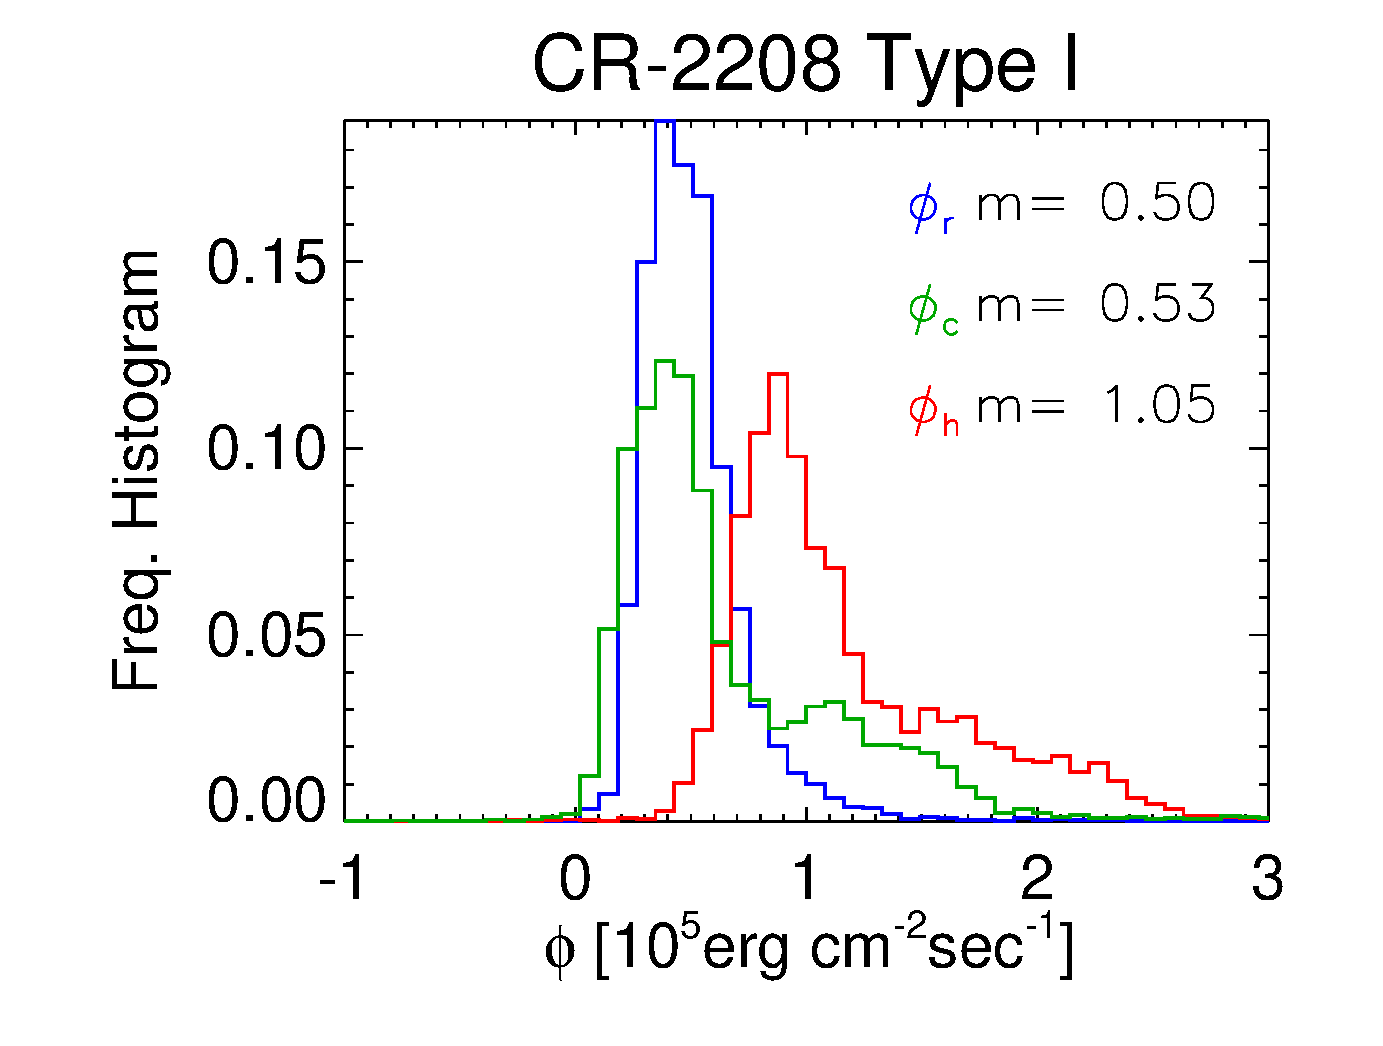
\includegraphics[width=0.495\textwidth]{figs/histocr2208_ccenergia.eps}
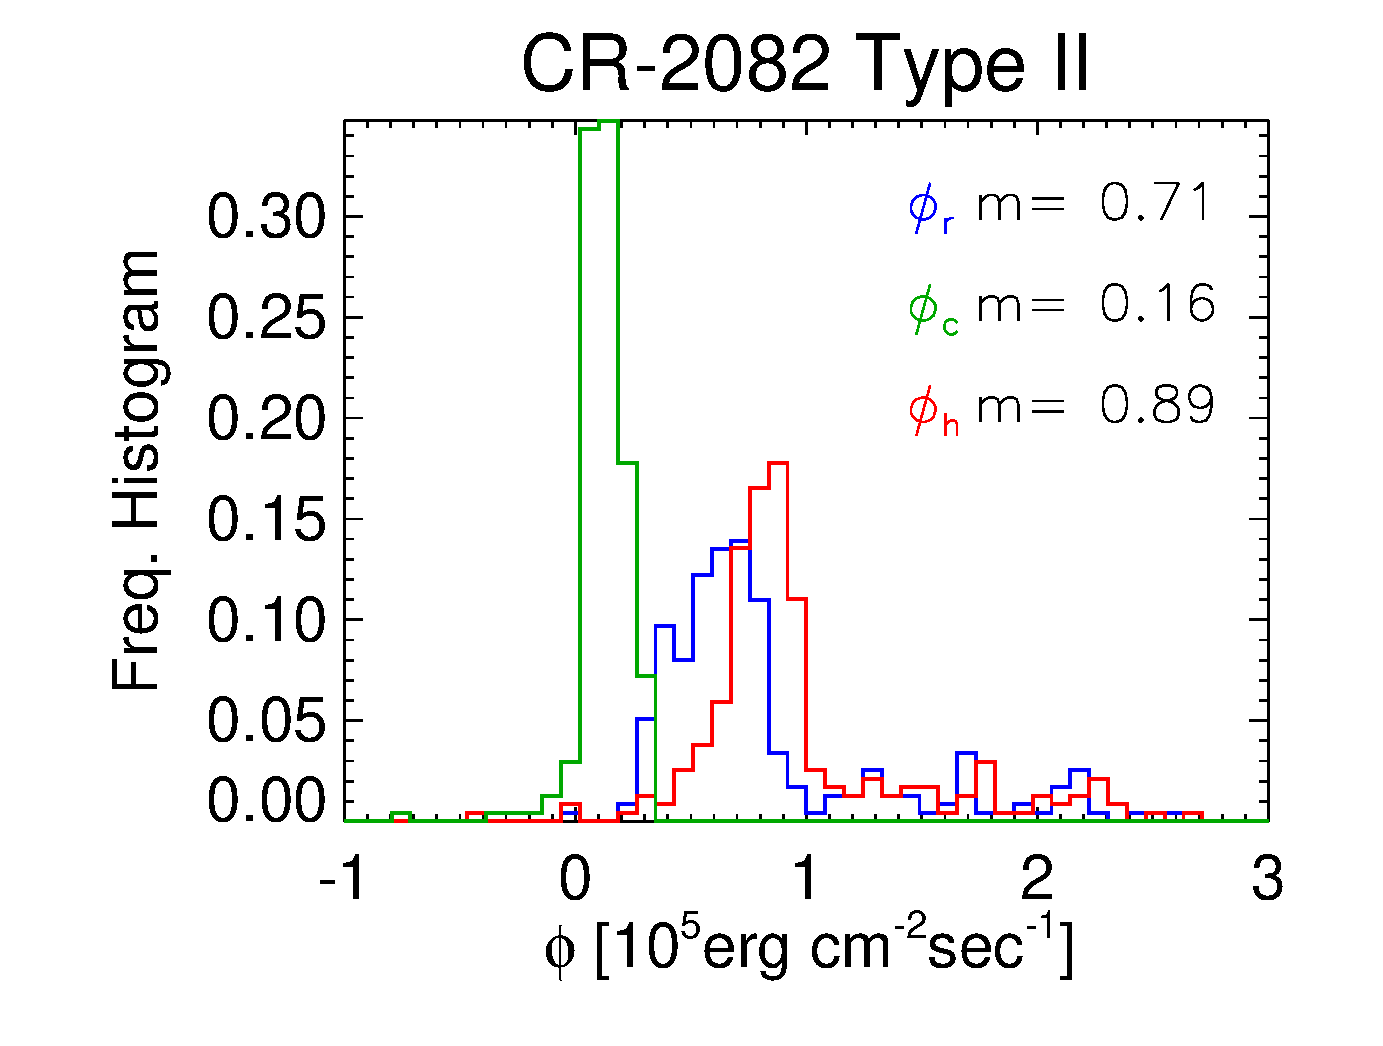
\includegraphics[width=0.495\textwidth]{figs/histocr2082_cgenergia.eps}
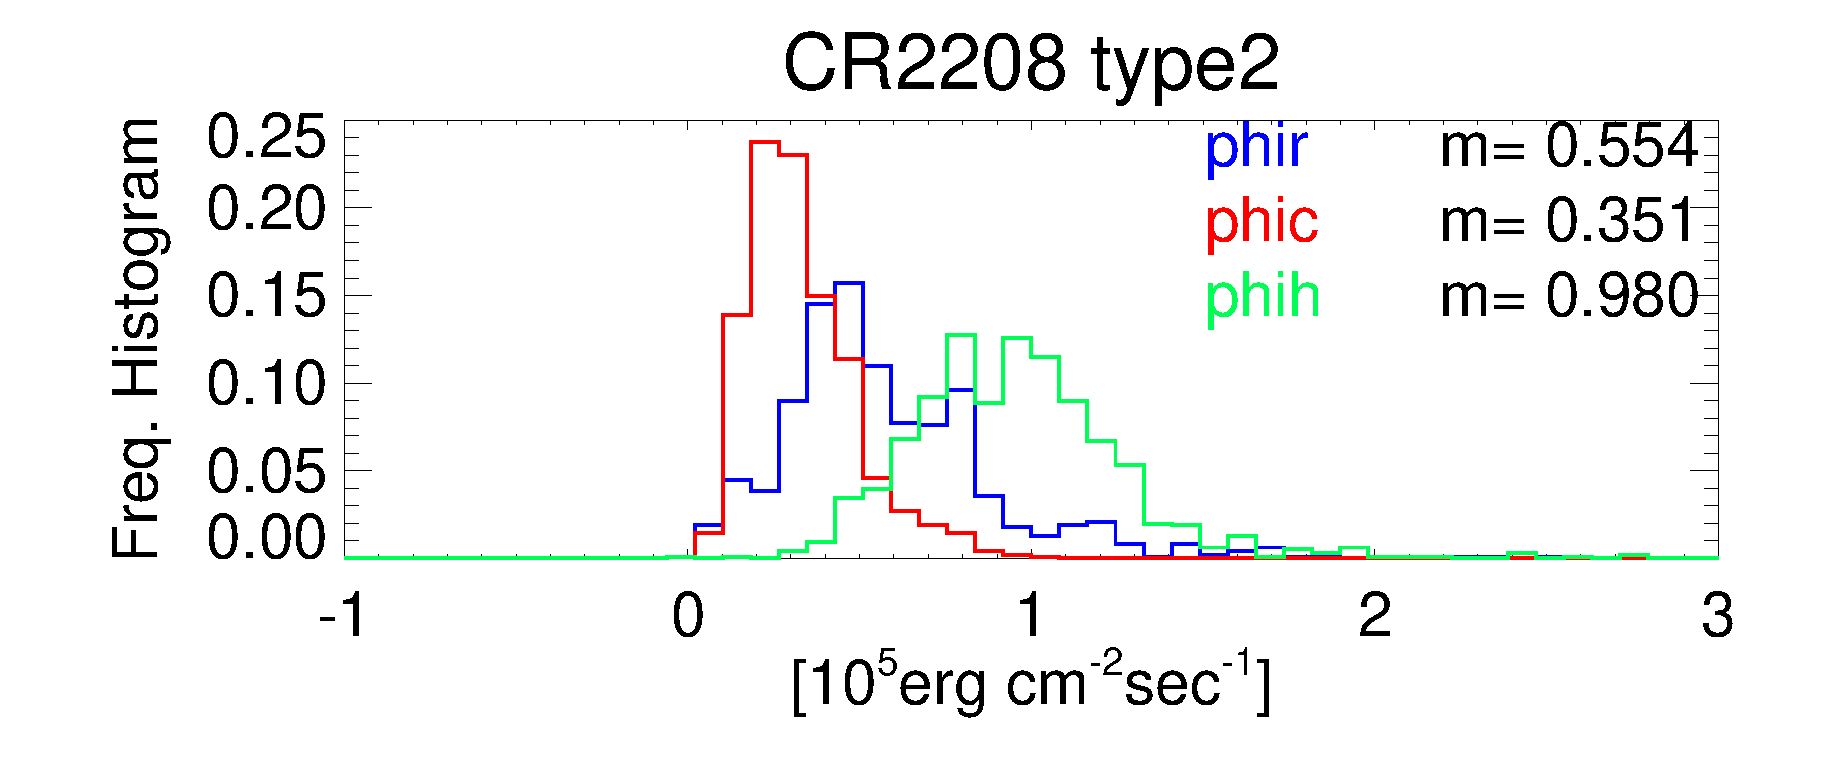
\includegraphics[width=0.495\textwidth]{figs/histocr2208_cgenergia.eps}
\caption{{Statistical results of the loop-integrated energy flux quantities $\phi_r,\phi_c,$ and $\phi_h$ in colors blue, red and green, respectively for CR-2082 (left) and CR-2208 (right). From top to bottom, panels show the results for loops of type 0, I and II, which are loops for which both legs meet the criteria from Section \ref{trace}.}}
\label{energia_demt}
\end{center}
\end{figure} 

{For both rotations, the value of the {loop-integrated} radiative power $E_r$, measured by the quantity $\phi_r$, is largest for loops of type 0. This is due to $E_r\propto N_e^2\,\Lambda(T_e)$, with both factors contributing to maximize $E_r$ for loops of type 0. As shown in Figure \ref{histos_fulldemt} and Table \ref{tabla_demt}, loops of type 0 are characterized by {the largest} values of electron density. Also, in the range of sensitivity of the EUVI and AIA instruments, namely 0.5–3.0 MK \citep{nuevo_2015}, the radiative loss function $\Lambda(T)$ has a local maximum at $\Tc\approx 1\,\MK$. According to Figure \ref{histos_fulldemt}, loops of type 0, I and II are characterized by {values of temperature that are progressively larger and farther} from the value $\Tc$, for both rotations.}

{{The sign of the quantity $\phi_c$ depends on that of the conductive flux $F_c$. Equations (\ref{Fc}) and (\ref{phi_c}) imply that } down loops (type 0) and up loops (type I and II) are characterized by $\phi_c<0$ and $\phi_c>0$, respectively, {as verified} in Figure \ref{energia_demt}.}

{{Adding the} radiative and conductive terms, the characteristic energy input flux at the coronal base is in the range $\phi_h\approx 0.5-1.5 \times 10^5\,\erg\,\cminvs\,\s^{-1}$, depending on the rotation and the type of {loop, matching the values reported by} \citet{maccormack_2017}. Note that for type 0 loops there is a marginal population characterized by the unphysical result $\phi_h<0$. As shown by \citet{maccormack_2017}, {this affects only the smallest sized loops of the type 0}, and it is {most probably} due to the limited temperature sensitivity of the instrumental passbands. The radiative loss term is {here calculated based on plasma emission detected by three coronal bands of EUVI or AIA. Though accounting for most of the coronal plasma, there surely is additional emission out of the instrumental sensitivity range. As a result,} the positive term $\phi_r$ is most likely underestimated, leading to values $\phi_h<0$ in loops of type 0, {being characterized by $\phi_c<0$. \vfill}} % NOTA el vfill

\subsection{{Comparison of the DEMT and AWSoM Models}}\label{awsom_res} 

%\noindent\notebyalbert{This section will show the results of AWSoM for $N_e$ and $T_e$, and how they compare with the corresponding results of DEMT ($\sqravgN$ and $\Tm$). It will first show the Carrington maps of $N_e$ and $T_e$ at the same three heights we showed the same maps for the DEMT results.  As the two targets are highly axis-symmetric, a first quantitative comparison between AWSoM and DEMT will be shown as longitude-averaged latitudinal profiles of the results of both models at a sample height. Then we will show the lat/lon location of loops of type I, II and III at a middle height, just loke for DEMT results. To make comparisons in distinct magnetic structures, we will show the average radial dependence of results for loops of type I, II and III, overplotting the AWSoM and the DEMT results. For the tree types of loops we will show histograms of the DEMT and AWSoM products along field lines. This is a LOT of information from which and we need to pull out a few clear conclusions.}

{For both target rotations,} Figures \ref{carmaps_awsom_2082} and \ref{carmaps_awsom_2208} show latitude-longitude maps of the AWSoM electron density and temperature. {Maps are shown} at the same three heights selected for visualization of the DEMT results in Figures \ref{carmaps_demt_2082} and \ref{carmaps_demt_2208}. {Thick-black curves} indicate the magnetic open/closed boundaries based on the magnetic field of the AWSoM model. Visual inspection of these maps shows that the AWSoM model for both rotations is highly {axisymetric}, as the tomographic model.

\begin{figure}[h!]
\begin{center}
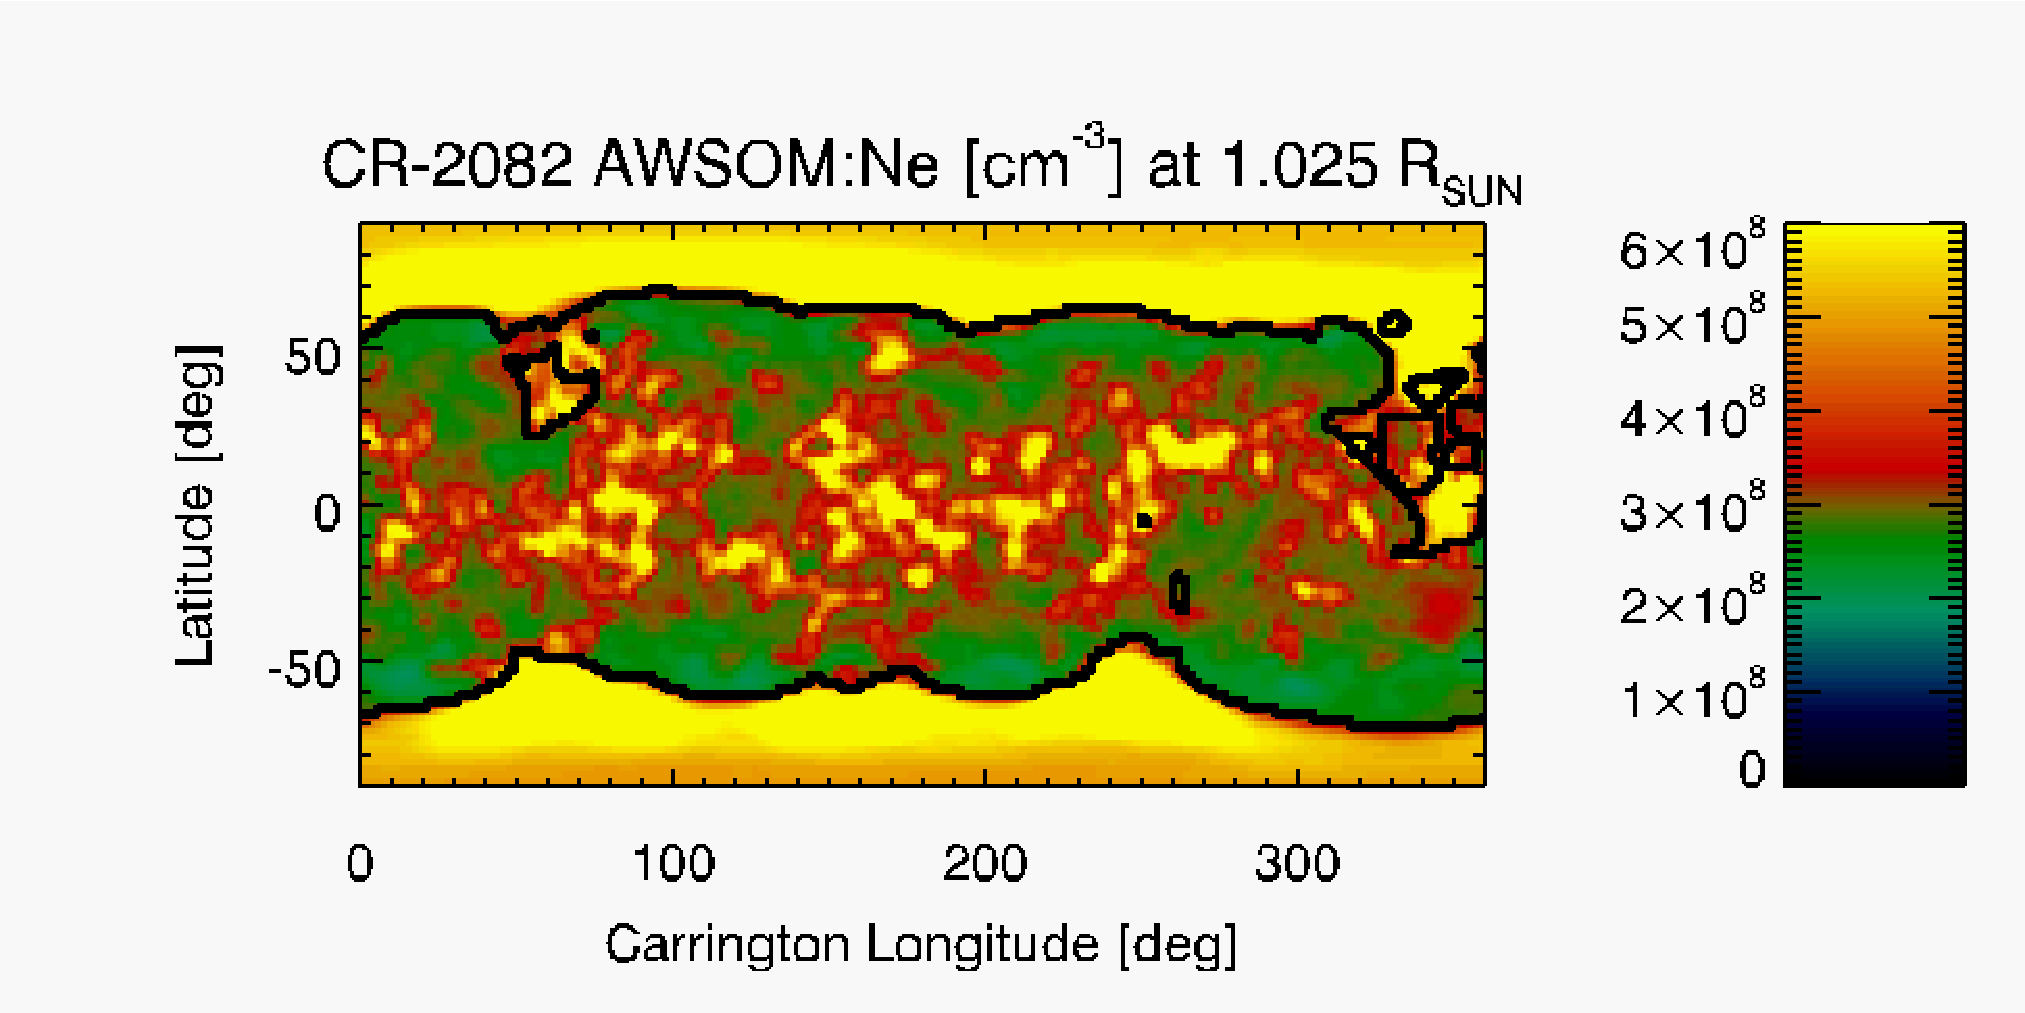
\includegraphics[width=0.495\textwidth]{figs/map_Ne_awsom_2082_185_short_1025_Rsun.pdf}
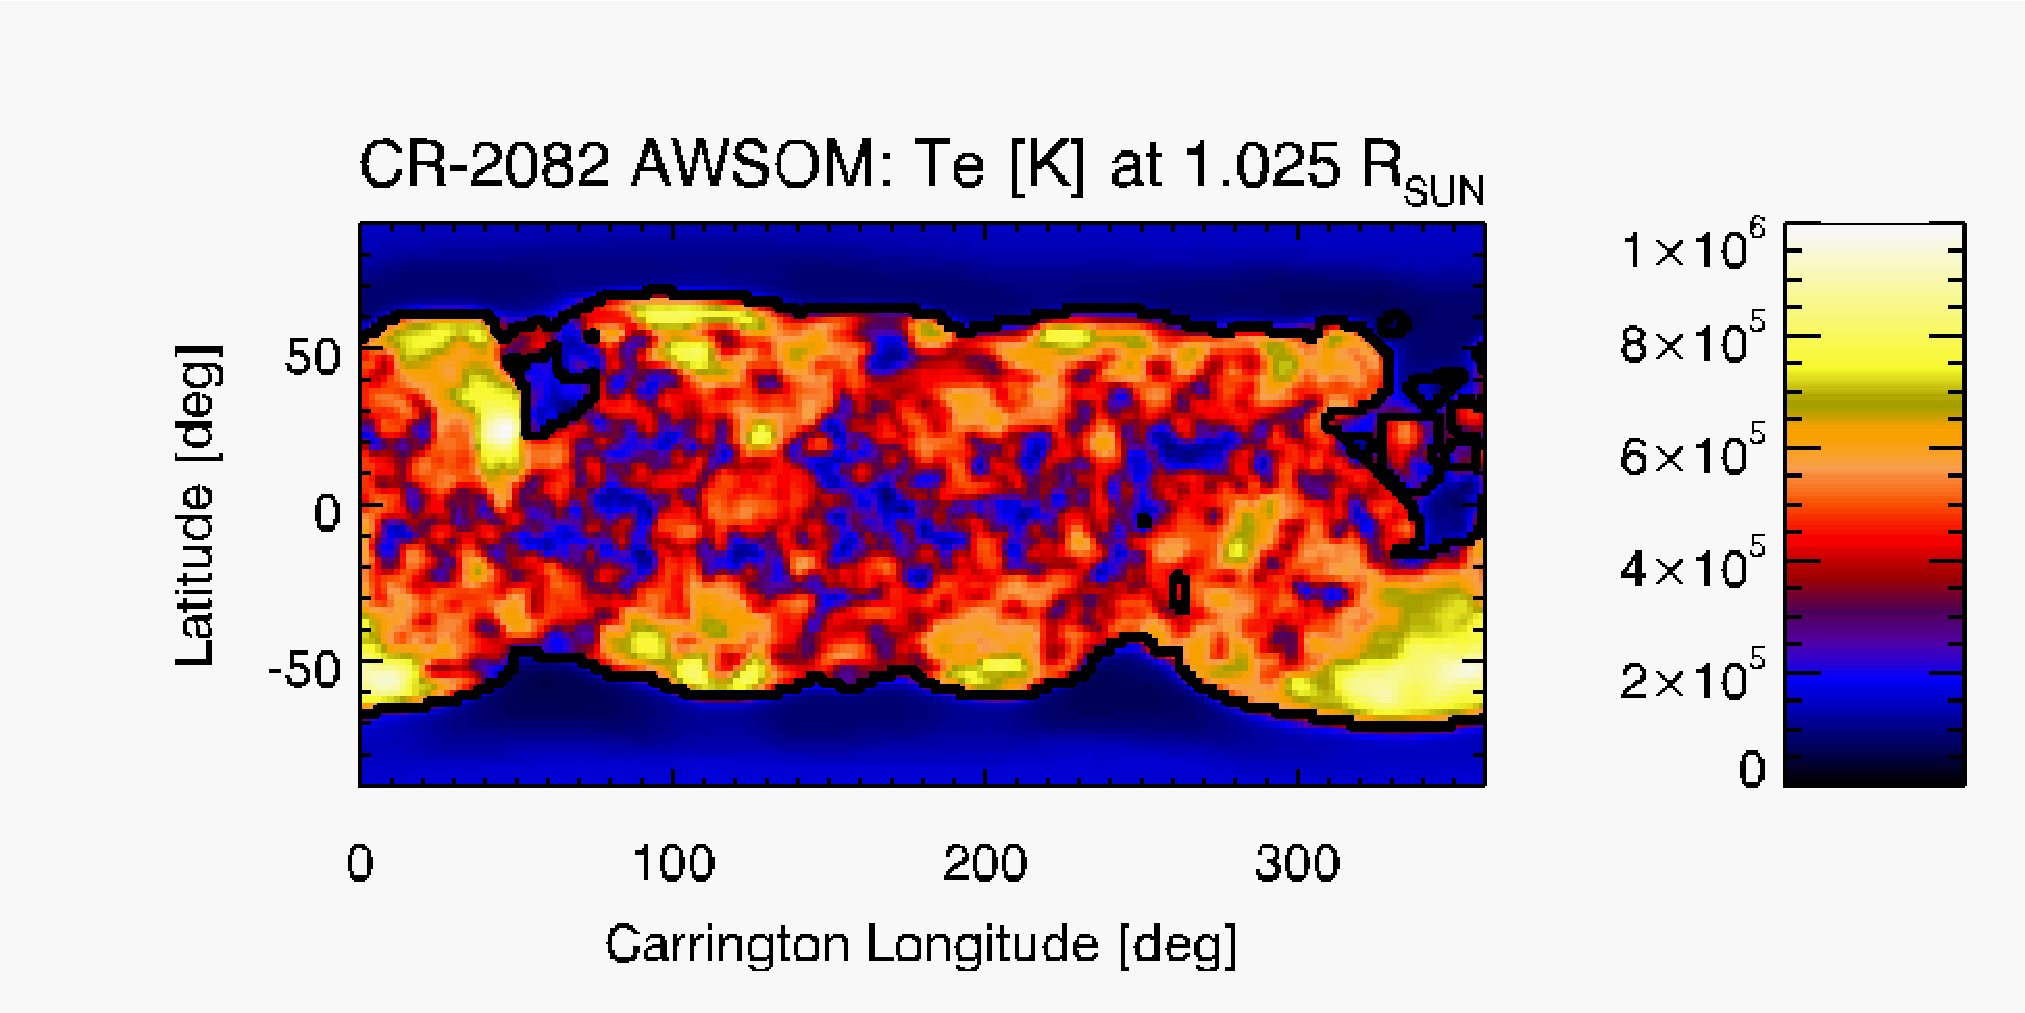
\includegraphics[width=0.495\textwidth]{figs/map_Te_awsom_2082_185_short_1025_Rsun.pdf}
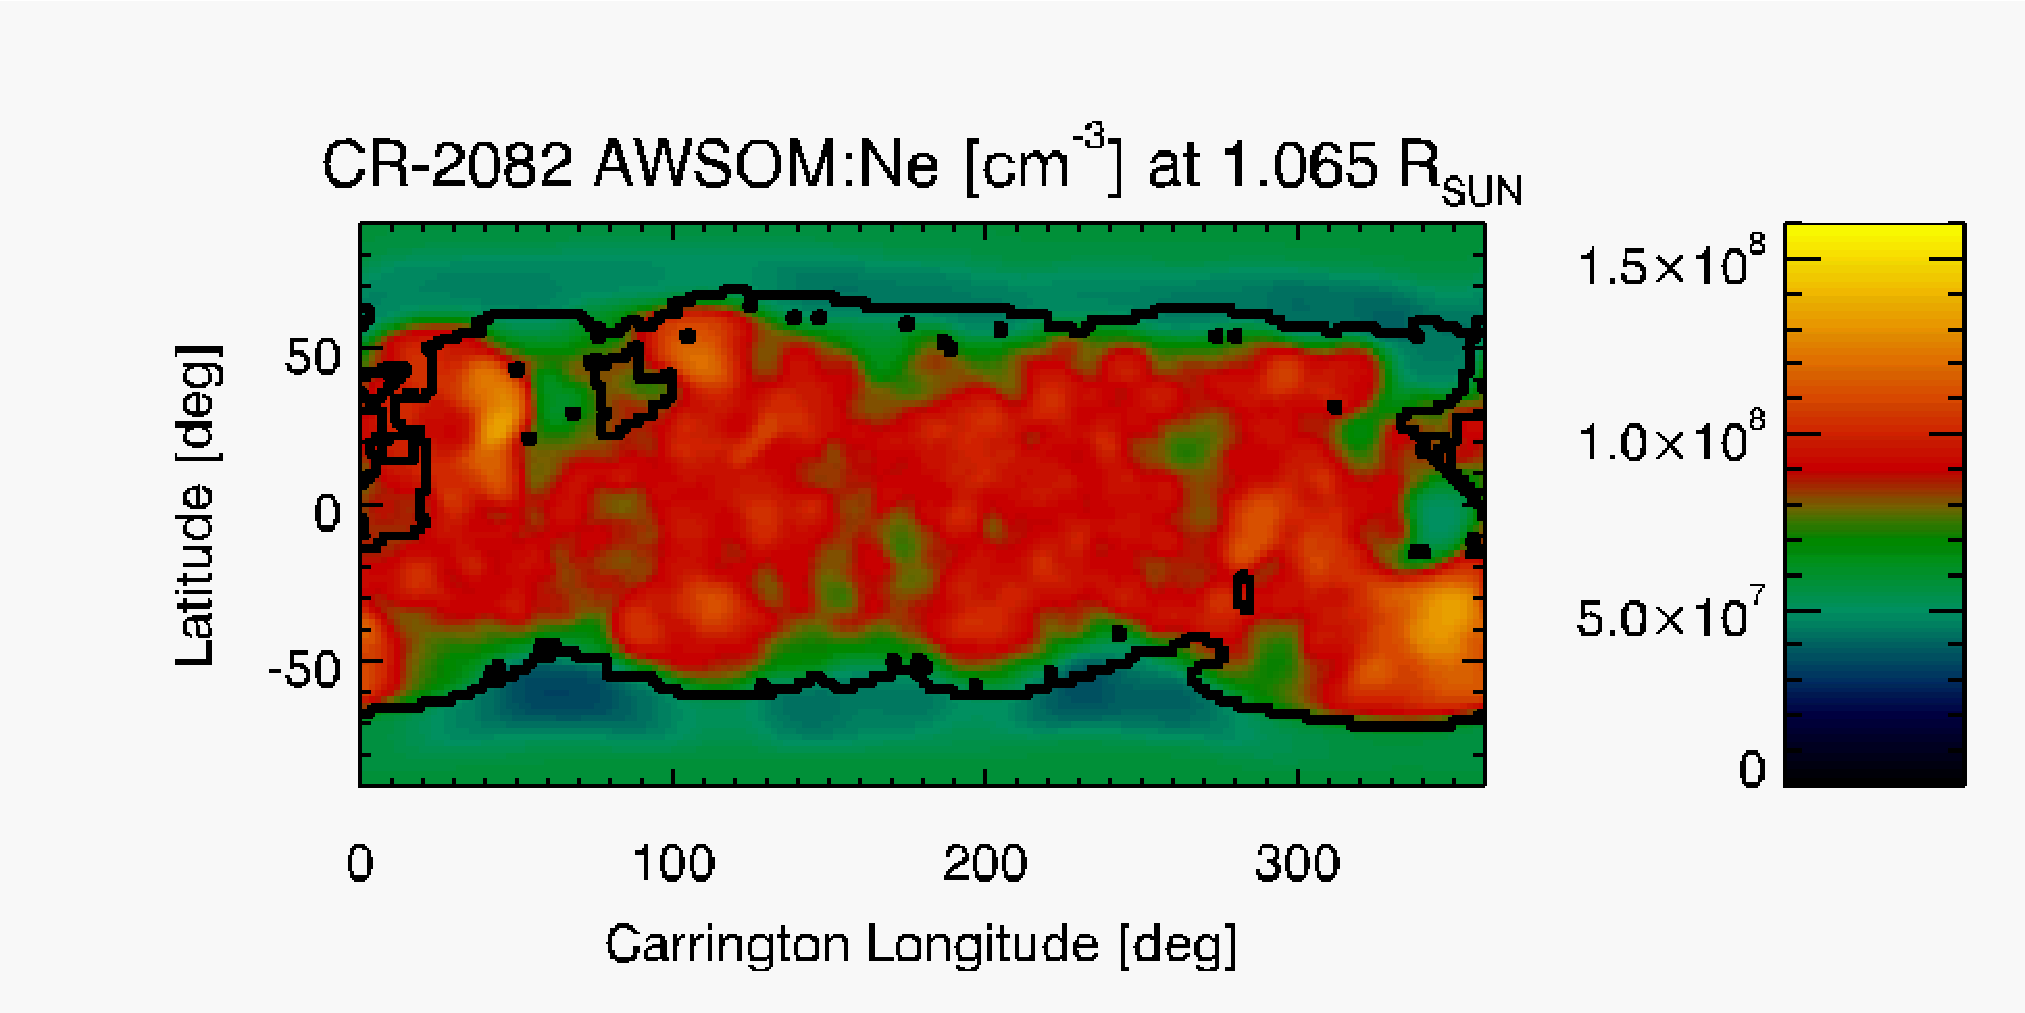
\includegraphics[width=0.495\textwidth]{figs/map_Ne_awsom_2082_185_short_1065_Rsun.pdf}
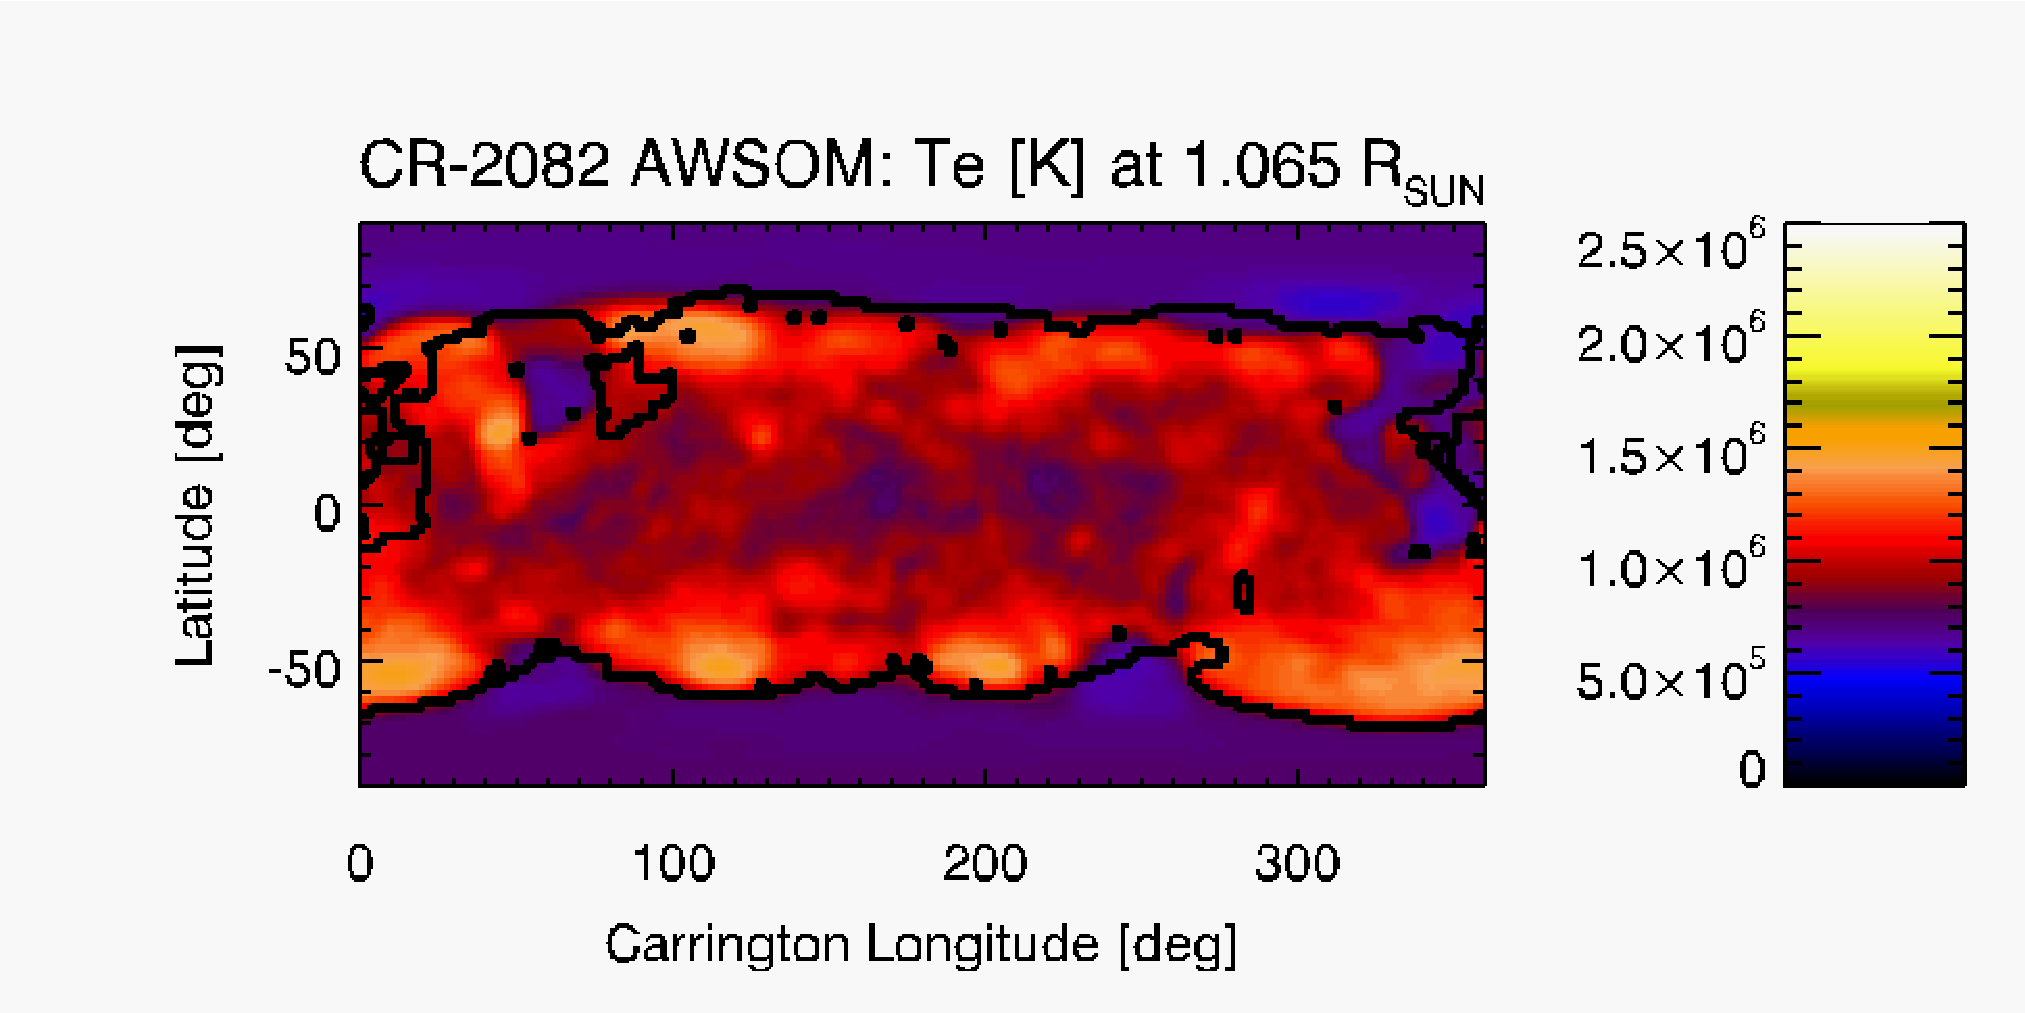
\includegraphics[width=0.495\textwidth]{figs/map_Te_awsom_2082_185_short_1065_Rsun.pdf}
\includegraphics[width=0.495\textwidth]{figs/map_Ne_awsom_2082_185_short_1105_Rsun.pdf}
\includegraphics[width=0.495\textwidth]{figs/map_Te_awsom_2082_185_short_1105_Rsun.pdf}
\caption{Carrington maps of density (left panels) and temperature (right panels) obtained with AWSoM model for the same three heights shown in Figure \ref{carmaps_demt_2082}.}
\label{carmaps_awsom_2082}
\end{center}
\end{figure}

{As described in Section \ref{awsom}, the AWSoM model includes an artificially thick TR, achieving coronal conditions above height $\approx 1.06\,\mrsun$. Indeed, the top panels in Figures \ref{carmaps_awsom_2082} and \ref{carmaps_awsom_2208}, at height $1.025\,\mrsun$, clearly do not represent coronal conditions (although we include them here for completeness). When compared to DEMT results (Figures \ref{carmaps_demt_2082} and \ref{carmaps_demt_2208}), the latitude-longitude maps of the AWSoM model for heights $1.065$ and $1.105\,\mrsun$ capture well the denser and hotter equatorial streamer belt surrounded by the less dense and colder CHs. Furthermore, for both target rotations, the temperature maps show the low latitudes of the equatorial streamer belt to be characterized by lower temperatures than its mid-latitudes, as also seen in the DEMT results. The latitude-longitude maps of the AWSoM and DEMT results are shown in the same units and scales, so that a visual comparison among them already reveals similar values of electron density and temperature in both models.}

\begin{figure}[h!]
\begin{center}
\includegraphics[width=0.495\textwidth]{figs/map_Ne_awsom_2208_185_short_1025_Rsun.pdf}
\includegraphics[width=0.495\textwidth]{figs/map_Te_awsom_2208_185_short_1025_Rsun.pdf}
\includegraphics[width=0.495\textwidth]{figs/map_Ne_awsom_2208_185_short_1065_Rsun.pdf}
\includegraphics[width=0.495\textwidth]{figs/map_Te_awsom_2208_185_short_1065_Rsun.pdf}
\includegraphics[width=0.495\textwidth]{figs/map_Ne_awsom_2208_185_short_1105_Rsun.pdf}
\includegraphics[width=0.495\textwidth]{figs/map_Te_awsom_2208_185_short_1105_Rsun.pdf}
\caption{Same as Figure \ref{carmaps_awsom_2208} for CR-2208.}
\label{carmaps_awsom_2208}
\end{center}
\end{figure}

{Being highly axisymmtric target rotations, the longitude-averaged latitudinal variation of the results of both models is an informative way to compare their large-scale structure. Such comparison is shown in Figure \ref{perf_lat} at height $1.105\,\mrsun$, with top panels comparing electron density and lower panels electron temperature. In these longitude-averaged profiles, longitudes containing ARs or low latitude CHs were excluded. In each panel the averaged latitudinal variation for the DEMT model is shown in solid-linestyle, while the result for the AWSoM model is shown in dashed-linesyle. Left panels show the comparison for CR-2082 (in blue) and right panels for CR-2208 (in red). In each panel the vertical black lines denote the corresponding longitude-averaged latitude of the open-close boundary in both hemispheres.}

\begin{figure}[h!]
\begin{center}
\includegraphics[width=0.495\textwidth]{figs/Perfil_Ne_demt_awsom_2082_1105.eps}
\includegraphics[width=0.495\textwidth]{figs/Perfil_Ne_demt_awsom_2208_1105.eps}
\includegraphics[width=0.495\textwidth]{figs/Perfil_Te_demt_awsom_2082_1105.eps}
\includegraphics[width=0.495\textwidth]{figs/Perfil_Te_demt_awsom_2208_1105.eps}
\caption{Longitude-averaged latitudinal dependence of the electron density (top) and temperature (bottom) for DEMT (blue) and AWSoM (red) results at $1.105\,\mrsun$. The left (right) panels correspond to CR-2082 (CR2208). The vertical black line indicates the longitude-averaged latitudes of the open/close magnetic boundary in both hemispheres.}
\label{perf_lat}
\end{center}
\end{figure}

{Several details from Figure \ref{perf_lat} are worth being highlighted. Firstly, for CR-2082 the electron density of both models agree within $\approx 20\%$ at all latitudes, and for CR-2208 the agreement is within $\approx5\%$. In the case of the electron temperature both models agree within $\approx 10-15\%$ at all latitudes for both target rotations. Secondly, for both target rotations, and for both models, these plots clearly show the relatively lower temperatures characterising the low-latitudes of the equatorial streamer belt compared to its mid-latitudes. Thirdly, for both target rotations, the latitude of the open/close magnetic boundary in both hemispheres matches the location of the strongest latitudinal gradient of the DEMT electron density. Note this is not the case for the AWSoM model, that shows a minimum density at the open/closed boundary. Last, note that the DEMT electron density decreases from the open/close boundary towards the poles (in both hemispheres of the two target rotations), while the AWSoM model shows the opposite trend.}

\begin{figure}[h!]
\begin{center}
\includegraphics[width=0.495\textwidth,clip=]{figs/Grispoint_2082_awsom_paper_test_Rpoint-map.pdf}
\includegraphics[width=0.495\textwidth,clip=]{figs/Grispoint_2208_awsom_paper_test_Rpoint-map.pdf}
\includegraphics[width=0.495\textwidth,clip=]{figs/Highpoint_2082_awsom_paper_cr2082_up_Rpoint-map.pdf}
\includegraphics[width=0.495\textwidth,clip=]{figs/Highpoint_2208_awsom_paper_cr2208_up_Rpoint-map.pdf}
\caption{Same as Figure \ref{rpoint_demt}, but using the density and temperature of the AWSoM model to classify {its legs in types I, II and III. The model does not exhibit legs of type 0.}}
\label{rpoint_awsom}
\end{center}
\end{figure} 

To characterize the results of the AWSoM model in distinct magnetic structures, its results for electron density and temperature were traced along its magnetic field lines. For each field line leg, the results were then fit to Equations (\ref{Nfit}) and (\ref{Tfit}){, considering only data points above heliocentric height $1.055\,\mrsun$. We then classified the traced legs into types I, II and III, according to the criteria described in Section \ref{trace}.  Legs of type 0 are not included for AWSoM, as in its current implementation it can not simulate down loops, a point we will discuss in the next section.}

\begin{figure}[h!]
\begin{center}
\includegraphics[width=0.31\textwidth,clip=]{figs/histo_2082_demt_awsom_streamer_up_ne_1055.eps}
\includegraphics[width=0.31\textwidth,clip=]{figs/histo_2082_demt_awsom_streamer_up_lambda_n.eps}
\includegraphics[width=0.31\textwidth,clip=]{figs/histo_2082_demt_awsom_streamer_up_Tm.eps}
\includegraphics[width=0.31\textwidth,clip=]{figs/histo_2082_demt_awsom_bound_up_ne_1055.eps}
\includegraphics[width=0.31\textwidth,clip=]{figs/histo_2082_demt_awsom_bound_up_lambda_n.eps}
\includegraphics[width=0.31\textwidth,clip=]{figs/histo_2082_demt_awsom_bound_up_Tm.eps}
\includegraphics[width=0.31\textwidth,clip=]{figs/histo_2082_demt_awsom_CH_up_ne_1055.eps}
\includegraphics[width=0.31\textwidth,clip=]{figs/histo_2082_demt_awsom_CH_up_lambda_n.eps}
\includegraphics[width=0.31\textwidth,clip=]{figs/histo_2082_demt_awsom_CH_up_Tm.eps}
\caption{{Statistical distribution {of the results of the DEMT (solid line-style) and AWSoM (dashed-linestyle) models} traced along legs of type I, II and III (from top to bottom), as defined in {Section \ref{trace}.} From left to right: electron density at the lowest coronal height of the AWSoM model $\Ne(r=1.055\,\mrsun)$, electron density scale height $\lN$, and leg-averaged electron temperature $\aTm$. In each panel the median {values $m$ are} indicated.}}
\label{histos_2082}
\end{center}
\end{figure} 

{For both target rotations, the top panels of Figure \ref{rpoint_awsom} show the latitude-longitude location (at heliocentric height $1.105\,\mrsun$) of all traced field line legs for which criterion (i) of Section \ref{trace} is met. That criterion is adapted here, requiring that at least five voxels of the tomographic grid are threaded by the leg. Open legs are indicated in gray color and closed ones in black color. For each leg, the fits to tomografic temperature and density were applied, as given by Equations \ref{Nfit} and \ref{Tfit}. Considering the AWSoM data points and the resulting fits along each leg, the bottom panels of Figure \ref{rpoint_awsom} show the latitude-longitude location of the subset for which also both criteria (ii) and (iii) of Section \ref{trace} are met. Using a three-color code, type I, II and III legs are shown in red, magenta and cyan color, respectively. This figure is to be compared with the corresponding Figure \ref{rpoint_demt} for DEMT results. It is readily seen that the AWSoM maps are more populated than those of DEMT. This is due to the 3D MHD model having electron density and temperature fields spatially smoother than those of DEMT.}

{For target rotation CR-2082, Figure \ref{histos_2082} shows the statistical distribution of the results of the DEMT (solid line-style) and AWSoM (dashed line-style) models traced along legs of type I, II and III (from top to bottom), as defined in Section \ref{trace}. From left to right: electron density at the lowest coronal height of the AWSoM model $\NCB\equiv\Ne(r=1.055\,\mrsun)$, electron density scale height $\lN$, and leg-averaged electron temperature $\aTm$. In each panel the median values $m$ are indicated. Figure \ref{histos_2208} shows the same analysis for target rotation CR-2208.}

\begin{figure}[h!]
\begin{center}
\includegraphics[width=0.31\textwidth,clip=]{figs/histo_2208_demt_awsom_streamer_up_ne_1055.eps}
\includegraphics[width=0.31\textwidth,clip=]{figs/histo_2208_demt_awsom_streamer_up_lambda_n.eps}
\includegraphics[width=0.31\textwidth,clip=]{figs/histo_2208_demt_awsom_streamer_up_Tm.eps}\\
\includegraphics[width=0.31\textwidth,clip=]{figs/histo_2208_demt_awsom_bound_up_ne_1055.eps}
\includegraphics[width=0.31\textwidth,clip=]{figs/histo_2208_demt_awsom_bound_up_lambda_n.eps}
\includegraphics[width=0.31\textwidth,clip=]{figs/histo_2208_demt_awsom_bound_up_Tm.eps}\\
\includegraphics[width=0.31\textwidth,clip=]{figs/histo_2208_demt_awsom_CH_up_ne_1055.eps}
\includegraphics[width=0.31\textwidth,clip=]{figs/histo_2208_demt_awsom_CH_up_lambda_n.eps}
\includegraphics[width=0.31\textwidth,clip=]{figs/histo_2208_demt_awsom_CH_up_Tm.eps}
\caption{Same as Figure \ref{histos_2082} for CR-2208.}
\label{histos_2208}
\end{center}
\end{figure} 

{For the two target rotations, Table \ref{tabla_comp} summarizes a quantitative comparative analysis between the results of the DEMT and AWSoM models {based on the results shown in Figures \ref{histos_2082} and \ref{histos_2208}}. The DEMT results are expressed as absolute values, while the ASWSoM results are informed as a percentual variation relative to the corresponding result for DEMT. The following major results can be drawn.}

{For target rotation CR-2082, the median value of the electron density $\NCB$ of both models agree within $\approx 10-25\%$, depending of the type of leg, while the median value of the scale height $\lN$ agree within $\approx 10\%$. The leg-averaged electron temperature $\aTm$ of both models also agree within $10\%$. For target rotation CR-2208 the agreement of the median value of $\NCB$ and $\lN$ of both models is within $5\%$, while median values of $\aTm$ agree within $15\%$. These detailed results informed per magnetic structure are fully consistent with the large-scale comparison provided in Figure \ref{perf_lat}.}

\begin{table}
\begin{tabular}{l r@{.}l@{\hskip 0.05in} r@{\hskip 0.01in} r  r@{.}l@{\hskip 0.05in} r@{\hskip 0.01in} r r@{.}l@{\hskip 0.05in} r@{\hskip 0.01in} r }
\hline
Type    & \multicolumn{4}{c}{$\med(\NCB)$}             & \multicolumn{4}{c}{$\med(\lN)$} & \multicolumn{4}{c}{$\med(\avgTe)$} \\
        & \multicolumn{4}{c}{$[10^8\,{\rm cm}^{-3}]$}  & \multicolumn{4}{c}{$[{\rm 10}^{-2}\,\mrsun]$} & \multicolumn{4}{c}{$[\MK]$} \\
\hline
CR-2082\\
I    & 1&15 &(\Mi&14\%)  &   7&5 &(\Pl&~8\%) &   1&25 &(\Mi&10\%) \\
II   & 0&99 &(\Mi&25\%)  &   9&9 &(\Mi&~2\%) &   1&36 &(\Mi&~2\%) \\
III  & 0&66 &(\Mi&17\%)  &   7&0 &(\Mi&~9\%) &   0&97 &(\Mi&~9\%) \\
\hline          
CR-2208\\
I    & 1&03 &(\Pl&~6\%)  &   9&7 &(\Mi&~8\%) &   1&55 &(\Mi&17\%) \\
II   & 0&79 &(\Pl&~9\%)  &  11&8 &(\Mi&14\%) &   1&58 &(\Mi&~8\%) \\
III  & 0&58 &(\Mi&~3\%)  &   8&9 &(\Mi&18\%) &   1&14 &(\Mi&18\%) \\
\end{tabular}
\caption{Median value (indicated as ``Md'') of the statistical distribution of $\NCB$, $\lN$, and $\aTm$ for each coronal type of lines defined in Section \ref{trace}. DEMT values are expressed in absolute terms, while AWSoM results are informed as a percentual variation relative to the corresponding DEMT value.}
\label{tabla_comp}
\end{table}

{Finally, to provide a graphical comparison of both models across the full range of heliocentric heights covered by the DEMT results, Figure \ref{perfiles_promedio} shows the average fits of $\Ne(r)$ and $T_e(r)$ for legs of type I (red), II (magenta), and III (cyan) for both target rotations. In each panel the DEMT and AWSoM results are plotted in solid and dashed linestyles, respectively.}

\begin{figure}[h!]
\begin{center}
\includegraphics[width=0.495\textwidth,clip=]{figs/perfil_paper_ne_cr2082_up.eps}
\includegraphics[width=0.495\textwidth,clip=]{figs/perfil_paper_te_cr2082_up.eps}
\includegraphics[width=0.495\textwidth,clip=]{figs/perfil_paper_ne_cr2208_up.eps}
\includegraphics[width=0.495\textwidth,clip=]{figs/perfil_paper_te_cr2208_up.eps}
\caption{{Average fits to $\Ne(r)$ (left panels) and $T_e(r)$ (right panels) for legs of {type I (red), II (magenta), and III (cyan)}, for CR-2082 (top panels) and CR-2208 (bottom panels). Solid lines correspond to DEMT results while dashed lines correspond to AWSoM results.}}
\label{perfiles_promedio}
\end{center}
\end{figure}

{As discussed above, Figure \ref{perf_lat} shows that the logitude-averaged latitudinal profile of the DEMT electron density in the CHs decreases towards the poles. Figure \ref{perf_lon_vr} below shows the longitude-averaged AWSoM radial wind speed $V_r$ at $6\,\mrsun$, where all field lines are open. The heliocentric current sheet (HCS) location is indicated by the minimum of the speed curve. For each rotation, all velocity data points to the south of the HCS position map down to the southern CH in Figures \ref{perf_lat}. Similarly, all velocity data points to the north of the HCS position map down to the northern CH in Figures \ref{perf_lat}. This clearly shows an anti-correlation between the DEMT electron density at low heights and the AWSoM wind speed at larger heights.}

\notebyalbert{We could quantify the anti-correlation between the AWSoM terminal speed and the DEMT electron density at the coronal base in the following fashion. We can set up starting points at, say, $20\,\mrsun$, every one degree, both in latitude and longitude. This would mean setting up $180\times 360$ starting points. We trace then the (open) field lines from each of those starting points down to $1.0\,\mrsun$ to find out the DEMT results at those lower heights for each field line. Now, to do this we need to develop some codes and have no time for this paper. We can postpone it for a next effort, or... Chip: do you think you could do this with your present tools? Do you think it is interesting? I think so. Our submission deadline is end-of-January.}

\begin{figure}[h!]
\begin{center}
\includegraphics[width=0.495\textwidth]{figs/Perfil_Vr_2082_5995.eps}
\includegraphics[width=0.495\textwidth]{figs/Perfil_Vr_2208_5995.eps}
\caption{{Longitude-averaged latitudinal dependence of the AWSoM model wind speed at $6.0\,\mrsun$ for CR2082 (left panel) and CR2208 (right panel).} \notebyalbert{(by Albert): Even if this is not yet the terminal speed, it is a pretty high height, and one can already see the transition from FAST to SLOW speed in the model, where the absolute minimum indicates the location of the HCS at this height. I believe it is interesting to compare these two curves with Figure 10. Note that while in this Figure all latitudes are magnetically open, in Figure 10 only the part at latitudes larger than the vertical black lines are open. Note that DEMT shows that in the open low corona $N_e$ decreases from the O/C boundary towards the poles, anti-correlating with the AWSoM terminal speed, which is nice. In order to quantify this anti-correlation we need to trace the terminal speed and the DEMT $N_e$, which we may need to do with the help of Chip and Nishtha. Chip, we can discuss this idea over Skype after Xmas if you are around.}}
\label{perf_lon_vr}
\end{center}
\end{figure}

\section{{Discussion and Conclusions}}\label{discu} 

\notebyalbert{Propongo que Diego escriba una primer sección limpia, ordenada. Lo que vos mandarías al Solar Physics, sin asteriscos ni nada raro. Expresate con párrafos limpios. Si querés destacar algo para discutir ponelo como una nota en rojo al final del párrafo correspondiente, no en el medio de los mismos. Yo creo que esto debe estructurarse así: 
\begin{enumerate}
\item Un párrafo (breve) de que se hizo, esto contextualiza. 
\item Dos o tres párrafos sobre los resultados 3.1. Esto es: resultados per se de cada rotación y como comparan (mencionando el tema incertezas). Estructura 3D del streamer en CAPAS, revelada observacionalmente en forma global por DEMT, esto incluye UP/DOWN loops. Explicar que con AIA no andamos bien en CHs. O sí? Energía.
\item Uno o dos párrafos sobre los resultados 3.2. Como compara AWSoM con DEMT. En forma breve. Vale la pena explicar que DOWN loops no se puede.
\item Luego un párrafo sobre next steps. Esto puede incluir nuevas cosas con AIA-4, el Eclipse, otras rotaciones de mayor intensidad.
\end{enumerate}
}

\notebyalbert{Este párrafo que sigue es de Albert. Algo así debe ir incluído dentro de la parte que refiere a 3.1. Creo que hay que corregir números a la luz de los análisis finales. Creo que los números de cuanto más frío o caliente, etc, deben ser corregidos a la luz de la nueva Tabla 1.}


In this work the combination of DEMT reconstructions and PFSS models has been used to perform a comparative study of the 3D thermodynamical state of the low solar corona ($1.02-1.23\,\mrsun$) {for two rotations sampling} the last two solar minima. Specifically the study compares rotations CR-1915 and CR-2081, {respectively sampling} the SC 22/23 and SC 23/24 minima. The SC 22/23 minimum was shorter, more active and intermittent. The SC 23/24 minimum {was remarkably} characterized by a $\approx 1$ year period {showing virtually} no sunspots. Being CR-2081 near the end of that extremely quiet period, it was one of the most axisymmetric and quiet rotations on record from that period \citep{nuevo_2013}.


In comparing the DEMT results obtained for the two selected targets, it is important to bear in mind they rely on data provided by two different instruments: AIA and EUVI. In order to quantify the systematic difference of the DEMT products based on both instruments, \citet{nuevo_2015}, who were the first to apply DEMT to AIA data, {analysed} a single target using both instruments independently. They found that while the density product is essentially equal, the temperature product of DEMT based on AIA data is systematically 8\% larger than the one based on EUVI data, i.e. $\Tm^{\rm(AIA)}/\Tm^{\rm(EUVI)} \approx 1.08$. Considering such correction, Figure \ref{histos_fulldemt} and Table \ref{tabla_demt} indicate that CR-2208 was $\approx 10-15\%$ hotter than CR-2082 throughout the streamer belt region. As for the electron density products, CR-2208 was found to be $\approx 15-20\%$ less dense than CR-2082 throughout the streamer belt region. These systematic differences are beyond the uncertainty level in the DEMT products due to systematic sources (radiometric calibration and tomographic regularization), that \citet{lloveras_2017} estimated to be $\lesssim 5\%$ and $\approx 2\%$ for the electron temperature and density, respectively. \notebyalbert{son estos errores compatibles con los informados en la Sección 2?}

\notebyalbert{El texto hasta el final son de Diego. Algunos se pueden ir, otros pueden servir de semilla para construir las distintas partes de la Sección.}

*We found down legs in the DEMT reconstructions mainly in the equatorial latitudes, being a greater quantity and better distribution along longitudes in CR-2082 than in CR-2208. \citet{nuevo_2013} showed a decrease in the amount of down loops as the solar activity increases, which is consistent with the results shown in this article.

*We can see, on type 0 loops, a median value of energy input flux ($\phi_h$) for CR-2082 twice bigger than CR-2208. In both rotations this magnitude has negative values, this can refer to some loops where loop-integrated radiative flux $\phi_r$) is too small in comparison with the larger gradients of negative conductive flux $\phi_c$), resulting in negative energy input flux. 

This effect can be due a subestimation of the density present in the loop or the limited range of temperature used to reconstruct tomographic parameters, that can affect the compute of radiative power. Nevertheless, this population represent lower than the \diego{ALGÚN PORCENTAJE$\%$} of total population in both cases.

Consistent that the density in CR-2082 was higher, the $\phi_r$ was also higher. In both rotations the magnitudes in the temperature gradients are similar, but the temperatures in CR-2208 were consistently higher at all heights, resulting in a larger $\phi_c$ in module. This results are in agree with the observations of \citet{maccormack_2017}.

\diego{THE AR of CR-2082 wasn't well modeled by AWSoM.}

In both rotations, AWSoM and DEMT resutls shows same termodynamic structures along latitude and longitude with very comparable values between $1.055 - 1.25\,\mrsun$

Figure \ref{histos_2082} and Table \ref{tabla_comp} indicate that AWSoM reconstruction of CR-2082 was found to be less dense $\approx 11-22\%$ and colder $\approx 5-10\%$.

Both reconstructions of CR-2208 reconstructed the ARs with very similare values and in almost the same latitude-longitude location. Figure \ref{histos_2208} and Table \ref{tabla_comp} indicate that AWSoM reconstruction of CR-2208 was found to be denser $\approx 0-10\%$ and colder $\approx 10-15\%$.

CR-2208 was $\approx 10-15\%$ hotter than CR-2082 throughout the streamer belt region. As for the electron density products, CR-2208 was found to be $\approx 15-20\%$ less dense than CR-2082 throughout the streamer belt region. These systematic differences are beyond the uncertainty level in the DEMT products due to systematic sources (radiometric calibration and tomographic regularization), that \citet{lloveras_2017} estimated to be $\lesssim 5\%$ and $\approx 2\%$ for the electron temperature and density, respectively.

\diego{I would like to say something about FIgure 10. Maybe the weird tale in AWSoM Ne in the poles. Ideas?}\\

%\diego{We could say something about the anti correlation between speed and density and not get into the trace because issues do always appear and we don't have much time, and we all want to be happy in january. Unless the collaborators find easy to make this part.}

%% Figure 
%
% \begin{figure} 
% \centerline{\includegraphics[width=0.5\textwidth,clip=]{<fig.eps>}}
% \caption{}%\label{fig:?}
% \end{figure}



%% Table
%
% \begin{table}
% \caption{}%\label{tbl:?}
% \begin{tabular}{}     
% \hline
% \multicolumn{2}{c}{<>}
% <data>
% \hline
% \end{tabular}
% \end{table}
  

%%%%%%%%%%%%%%%%%%%%%%%%%%%%%%%%%%%%%%%%%%%%%%%%%%%%%%%%%%%%%%%%%%%%%%%%%%%
%% Appendix
%
% \appendix   



%%%%%%%%%%%%%%%%%%%%%%%%%%%%%%%%%%%%%%%%%%%%%%%%%%%%%%%%%%%%%%%%%%%%%%%%%%%
%% Acknowledgements
%
% \begin{acks}
%
% \end{acks}


%%% %%%%%%%%%%%%%%%%%%%%%%%%%%%%%%%%%%%%%%%%%%%%%%%%%%%%%%%%%%%
%% Bibliography
%
% Using BibTeX
%
\bibliographystyle{spr-mp-sola}
\bibliography{solphys_dglloveras}  
%
% Without BibTeX 
% \begin{thebibliography}{}
% \bibitem[\protect\citeauthoryear{Author}{Year}]{key}
%   <bibliographical entry>
%
% \bibitem[\protect\citeauthoryear{}{}]{}
%   
%  
% \end{thebibliography}

\end{article} 
\end{document}
